\documentclass[11pt,a4paper,oneside]{report}

% --- PACKAGES DE BASE ---
\usepackage[utf8]{inputenc}
\usepackage[T1]{fontenc}
\usepackage[french]{babel}
\usepackage{lmodern}
\usepackage{microtype}
\usepackage{geometry}
\usepackage{eso-pic}
\usepackage{transparent}
\usepackage{lmodern}
\geometry{a4paper, total={160mm,245mm}, left=25mm, top=25mm}
\usepackage{setspace}
\setstretch{1.1}
\usepackage{float}
\usepackage{caption}
\usepackage{subfig}
\usepackage{amsmath, amssymb, amsfonts, mathrsfs}
\usepackage{algorithm}
\usepackage{algpseudocode}
\usepackage{tcolorbox}
\usepackage{longtable}
\usepackage{enumitem} 
\usepackage{amsthm}
\usepackage{tikz}
\usepackage{tikz-3dplot}
\usetikzlibrary{3d, angles, quotes, positioning, decorations.pathreplacing, matrix, fit, arrows.meta, calc}
\usepackage{shorttoc}
\usepackage[hidelinks]{hyperref}
\hypersetup{colorlinks=true, linkcolor=black, citecolor=blue, urlcolor=blue}
\usepackage{booktabs}

\theoremstyle{plain}
\newtheorem{proposition}{Proposition}[chapter]

\renewcommand{\proofname}{Démonstration}

\usepackage{graphicx}

\usepackage{fancyhdr}
\pagestyle{fancy}
\fancyhf{}
\renewcommand{\headrulewidth}{0.4pt}
\fancyhead[L]{\textit{\nouppercase{\leftmark}}}
\fancyhead[R]{\thepage}

\usepackage{titlesec}
\titleformat{\chapter}[hang]{\huge\bfseries}{\thechapter\quad}{0pt}{}
\titlespacing*{\chapter}{0pt}{-20pt}{20pt}

\makeatletter
\def\clap#1{\hbox to 0pt{\hss #1\hss}}
\def\haut#1#2#3{\hbox to \hsize{\rlap{\vtop{\raggedright #1}}\hss \clap{\vtop{\centering #2}} \hss \llap{\vtop{\raggedleft #3}}}}
\def\bas#1#2#3{\hbox to \hsize{\rlap{\vbox{\raggedright #1}}\hss \clap{\vbox{\centering #2}} \hss \llap{\vbox{\raggedleft #3}}}}

\def\maketitle{%
\thispagestyle{empty}
\vbox to \vsize{%
    \haut{}{\@blurb}{}
    \vfill
    \hrule height 2pt \vspace{0.4cm}
    \begin{center}\huge \textbf{\@title}\end{center}
    \vspace{0.2cm} \hrule height 2pt \vspace{2cm}
    \begin{center}\Large \textit{Auteur :}\\ \textbf{\@author}\end{center}
    \vspace{1cm}
    \begin{center}\Large \textit{Responsable :}\\ \textbf{Stephane Marchand Maillet}\end{center}
    \vfill
    \bas{}{\begin{flushright} \large \@location \end{flushright}}{}
}\cleardoublepage}

\def\location#1{\def\@location{#1}}
\def\blurb#1{\def\@blurb{#1}}
\makeatother

\title{Sensibilité structurelle des réseaux convolutionnels aux directions des bases de Fourier}
\author{David Tournier Marrucho}
\location{\today}
\blurb{
    \begin{center}
        
\includegraphics[width=4cm]{formalisme/logo_unige.png} \\[1.5em]
        \textbf{Bachelor en Science Informatique} \\
        UNIGE - Faculté des Sciences - Département d'Informatique
    \end{center}
}

\begin{document}

\maketitle

\tableofcontents
\newpage

\onehalfspacing
% !TeX root = ../main.tex

\chapter*{Table des notations}
\addcontentsline{toc}{chapter}{Table des notations}

\renewcommand{\arraystretch}{1.35}
\small

\begin{longtable}{p{3cm} p{10.5cm}}
    \hline
    \textbf{Notation} & \textbf{Description} \\
    \hline
    \endfirsthead

    \hline
    \textbf{Notation} & \textbf{Description} \\
    \hline
    \endhead

    \hline
    \endfoot

    \multicolumn{2}{l}{\textbf{Indices, images et fréquences}} \\
    \hline
    $N$ & Taille spatiale des images considérées. Dans les expériences sur CIFAR, $N=32$. \\
    $\mathbb{Z}_N$ & Ensemble des indices $\{0,\dots,N-1\}$, interprétés modulo $N$. \\
    $(m,n)$ & Coordonnées spatiales d'un pixel : $m$ pour la direction verticale, $n$ pour la direction horizontale. \\
    $(u,v)$ & Fréquence de Fourier 2D : $u$ pour la fréquence verticale, $v$ pour la fréquence horizontale. \\
    $w(u,v)$ & Indice aplati associé à la fréquence $(u,v)$, utilisé après vectorisation. \\
    $x$, $X$, $Y$ & Image ou signal d'entrée, image d'entrée matricielle et image de sortie. \\

    \hline
    \multicolumn{2}{l}{\textbf{Fourier et convolution}} \\
    \hline
    $h$ & Filtre de convolution. \\
    $h_{i,j}$ & Filtre reliant le canal d'entrée $j$ au canal de sortie $i$. \\
    $*$ & Convolution circulaire. \\
    $\phi_k$ & Vecteur de Fourier discret 1D associé à la fréquence $k$. \\
    $\Phi_{u,v}$ & Onde de Fourier 2D associée à la fréquence $(u,v)$. \\
    $F_N$ & Matrice de Fourier 1D dont les colonnes sont les vecteurs $\phi_k$. \\
    $Q_N$ & Matrice de Fourier 2D vectorisée, définie par $Q_N = F_N \otimes F_N$. \\
    $\operatorname{vec}(X)$ & Vectorisation de l'image $X$ en empilant ses colonnes. \\
    $\lambda_f$, $\lambda^{i,j}_{u,v}$ & Valeurs propres associées à l'action d'un filtre de convolution sur une fréquence de Fourier. \\

    \hline
    \multicolumn{2}{l}{\textbf{Représentation matricielle du réseau}} \\
    \hline
    $I_r$ & Matrice identité de taille $r \times r$. En particulier, $I_N$ désigne l'identité de taille $N$, et $I_{m_k}$ l'identité agissant sur les canaux de la couche $k$. \\
    $M$ & Matrice représentant une couche de convolution, ou l'opérateur linéaire global selon le contexte. \\
    $M^{(k)}$ & Matrice représentant la $k$-ième couche de convolution de $\mathbb{C}^{m_kN^2}$ vers $\mathbb{C}^{m_{k+1}N^2}$. \\
    $m_{\mathrm{in}}$, $m_{\mathrm{out}}$ & Nombre de canaux d'entrée et de sortie d'une couche de convolution considérée isolément. \\
    $m_k$ & Nombre de canaux en entrée de la couche $k$. \\
    $L$ & Matrice décrivant les mélanges de canaux dans le domaine de Fourier. \\
    $G^{(w)}$ & Matrice de mélange associée à une fréquence donnée $w$. \\
    $\sigma$ & Valeur singulière, utilisée pour mesurer l'amplification d'une direction d'entrée. \\
    $a$, $b$ & Vecteurs singuliers droit et gauche associés à une fréquence donnée. \\

    \hline
    \multicolumn{2}{l}{\textbf{Perturbations et protocole expérimental}} \\
    \hline
    $\epsilon$ & Amplitude maximale autorisée pour la perturbation, mesurée en norme $\ell_\infty$. \\
    $p_{u,v}$ & Motif spatial réel construit à partir de la fréquence $(u,v)$. \\
    $\delta_{u,v}$ & Perturbation de Fourier normalisée associée à la fréquence $(u,v)$. \\
    $\tilde{x}$ & Image perturbée obtenue après ajout de $\delta_{u,v}$ puis clipping dans $[0,1]$. \\
    $f$ & Modèle de classification étudié. \\
    $\mathcal{D}$ & Ensemble d'images utilisé pour l'évaluation. \\
    $\operatorname{FR}(u,v)$ & \textit{Fool ratio} obtenu pour la fréquence $(u,v)$, c'est-à-dire la proportion de prédictions modifiées. \\
    $H$ & Heatmap de sensibilité fréquentielle contenant les valeurs de $\operatorname{FR}(u,v)$. \\
    $(u^\star,v^\star)$ & Fréquence qui maximise le \textit{fool ratio}. \\

    \hline
\end{longtable}

\normalsize
\chapter{Introduction}

Les réseaux de neurones convolutionnels, souvent appelés CNN pour \textit{Convolutional Neural Networks}, 
inspirés par le cortex visuel des vertébrés, occupent une place centrale en vision par ordinateur. 
Ils sont utilisés pour reconnaître des objets, classer des images, détecter des formes ou encore extraire 
automatiquement des informations visuelles. 

Leur efficacité vient en grande partie de leur capacité à apprendre des motifs locaux dans les 
images, puis à les combiner progressivement pour construire des représentations plus abstraites. 

\section*{Fragilités et attaques adversariales}

Cependant, malgré leurs très bonnes performances, ces modèles peuvent présenter des fragilités structurelles. 
Une image peut être faiblement modifiée, de telle manière que cela devienne imperceptible à l'oeil humain, 
tout en entraînant un changement important dans la prédiction du réseau. Ce phénomène est connu sous le nom de 
\textbf{perturbation adversariale}~\cite{szegedy2014intriguing}.

Un aspect particulièrement intéressant de ces perturbations est leur caractère parfois universel. Dans certains cas, 
il est possible de trouver une perturbation qui est directement basée sur l'architecture du réseau 
(sa manière de fonctionner), exploitant une faiblesse structurelle du fonctionnement interne de ce dernier. 
Ainsi ce genre de perturbation, une fois trouvée, peut être appliquée à n'importe quelle image, 
\textbf{indépendamment} de son contenu, et tromper le modèle, pour une proportion importante d'images,
dans ses prédictions. On parle alors de perturbation adversariale \textbf{universelle}~\cite{moosavi2017universal}. 

La question centrale est alors de comprendre d'où vient cette sensibilité. Une première explication possible 
consiste à l'attribuer aux données d'entraînement ou à l'optimisation du modèle. Dans ce travail, nous nous 
intéressons à une autre piste : \textbf{la structure même des réseaux convolutionnels}. En effet, les CNN 
reposent sur des couches de convolution, et ces couches possèdent des propriétés mathématiques particulières. 

\section*{L'approche par la base de Fourier}

Pour étudier cette question, nous choisissons d'utiliser la base de Fourier. Une image peut être 
décrite pixel par pixel, mais elle peut aussi être décomposée en motifs fréquentiels : des variations lentes, 
des oscillations rapides, des motifs horizontaux, verticaux ou diagonaux. Ces motifs fréquentiels donnent une 
autre manière de décrire les structures présentes dans une image.

Ainsi, analyser une image non plus seulement dans le domaine spatial, c'est-à-dire à partir de ses pixels, mais 
aussi dans le domaine fréquentiel, permet de mieux comprendre quelles composantes de l'image influencent le 
comportement du réseau et quelles directions de perturbation peuvent devenir particulièrement sensibles.

Ce lien constitue le point de départ du travail de Tsuzuku et Sato~\cite{tsuzuku2019structural}, qui montrent 
que certains réseaux convolutionnels sont particulièrement sensibles à des directions issues de la base de Fourier. 
Leur idée est que certaines perturbations adversariales universelles peuvent être mieux comprises en étudiant la 
manière dont les couches convolutionnelles traitent les fréquences.

\begin{center}
    \vspace{1em}
    \rule{0.4\textwidth}{0.4pt} \\
    \vspace{1em}
    \begin{minipage}{0.85\textwidth}
        \centering
        \large \itshape
        Comment l'architecture convolutionnelle des CNN induit-elle des directions de vulnérabilité privilégiées dans 
        le domaine de Fourier, et dans quelle mesure cette sensibilité structurelle permet-elle de mieux comprendre 
        l'existence de perturbations adversariales universelles ?
    \end{minipage} \\
    \vspace{1em}
    \rule{0.4\textwidth}{0.4pt}
    \vspace{1em}
\end{center}

L'objectif de ce rapport est de reprendre cette idée et de la reconstruire petit à petit de manière plus détaillée en 
introduisant les éléments nécessaires pour comprendre les résultats, de telle manière que n'importe quel lecteur avec une connaissance 
de base en algèbre linéaire et en machine learning puisse comprendre les implications de ce travail.

\section*{Organisation du rapport}

Pour répondre à cette problématique, le rapport est organisé de la manière suivante :

\begin{itemize}[label=\textbullet, leftmargin=1.5cm]
    \item \textbf{Chapitre 2 :} Présentation du contexte général : réseaux convolutionnels, robustesse et perturbations adversariales.
    \item \textbf{Chapitre 3 :} Présentation des fondements théoriques reliant convolution et base de Fourier. 
    On y montre notamment l'émergence naturelle des fonctions de Fourier dans l'analyse linéaire.
    \item \textbf{Chapitre 4 :} Présentation de la reproduction expérimentale, du protocole utilisé, des \textit{heatmaps} 
    de sensibilité fréquentielle, puis discussion des résultats et des limites.
    \item \textbf{Conclusion :} Synthèse des enseignements et perspectives de recherche.
\end{itemize}

% % !TeX root = ../main.tex

% \chapter{Contexte}

% Ce chapitre introduit les notions nécessaires pour comprendre la suite du rapport. 
% L'objectif est de fixer le contexte général : ce qu'est un réseau convolutionnel, pourquoi la robustesse est une 
% question importante, et en quoi les perturbations adversariales motivent l'analyse menée dans ce travail.

% \section{Les réseaux convolutionnels en vision par ordinateur}

% En vision par ordinateur, une image peut être vue comme une grille de pixels. 
% Chaque pixel contient une information visuelle locale saisie par un capteur tel qu'un appareil photo, comme une intensité 
% lumineuse, dans le cas d'une image en niveaux de gris (image en noir et blanc) ou plusieurs valeurs dans le cas d'une image couleur, par exemple les canaux rouge, vert et bleu.
% Un modèle de classification d'images doit donc apprendre à transformer cette grille de valeurs en une prédiction, 
% comme une classe d'objet (par exemple, "chat" ou "chien") ou une catégorie visuelle (par exemple, "animal" ou "véhicule").

% Les réseaux de neurones convolutionnels, contrairement à un réseau entièrement 
% connecté (\textit{fully-connected}), qui traiterait tous les pixels comme des variables 
% indépendantes, exploite directement la structure spatiale de l'image. 
% Il analyse l'image localement, à l'aide de filtres appliqués sur de petites régions voisines, afin de détecter des motifs locaux comme des contours ou des textures. 
% En combinant ces motifs à travers plusieurs couches, le CNN peut construire des représentations de plus en plus abstraites,
% capables de reconnaître des objets complexes ou des catégories visuelles. La figure~\ref{fig:lenet5} illustre justement ce principe.

% \begin{figure}[H]
%     \centering
%     \resizebox{\textwidth}{!}{
%         \begin{tikzpicture}[
%             font=\sffamily\small,
%             map/.style={fill=gray!60, draw=gray!80, line width=0.5pt},
%             vector/.style={fill=gray!70, draw=none},
%             conn/.style={draw=black, thin},
%             rf/.style={draw=black, thick, fill=none}
%         ]
%     \filldraw[fill=gray!40, draw=none] (0,0) rectangle (3.2, 3.2);
%     \draw[line width=4pt, rotate around={15:(1.6,1.7)}] (1.6, 1.7) ellipse (0.7 and 1.1);
%     \node[above, align=center, font=\sffamily\small\bfseries] at (1.6, 3.8) {INPUT\\32x32};
%     \foreach \i in {5,4,...,0} {

%         \filldraw[map] (5.0 - \i*0.15, 0.2 + \i*0.15) rectangle +(2.8, 2.8);

%     }

%     \node[above, align=center] at (6.0, 3.8) {C1: feature maps\\6@28x28};
%     \foreach \i in {5,4,...,0} {

%         \filldraw[map] (9.0 - \i*0.15, 0.6 + \i*0.15) rectangle +(1.4, 1.4);

%     }
%     \node[above, align=center] at (9.3, 3.8) {S2: f. maps\\6@14x14};
%     \foreach \i in {15,14,...,0} {

%         \filldraw[map] (12.5 - \i*0.1, 0.8 + \i*0.1) rectangle +(1.0, 1.0);

%     }
%     \node[above, align=center] at (12.2, 3.8) {C3: f. maps\\16@10x10};
%     \foreach \i in {15,14,...,0} {

%         \filldraw[map] (15.5 - \i*0.1, 1.0 + \i*0.1) rectangle +(0.5, 0.5);

%     }
%     \node[above, align=center] at (15.0, 3.8) {S4: f. maps\\16@5x5};
%     \filldraw[vector] (18.5, 0.5) -- (18.9, 0.5) -- (16.9, 3.5) -- (16.5, 3.5) -- cycle;
%     \node[above, align=center] at (17.7, 3.8) {C5: layer\\120};
%     \filldraw[vector] (21.5, 0.7) -- (21.9, 0.7) -- (20.3, 3.1) -- (19.9, 3.1) -- cycle;
%     \node[above, align=center] at (20.9, 3.8) {F6: layer\\84};
%     \filldraw[vector] (24.5, 1.0) -- (24.9, 1.0) -- (23.9, 2.4) -- (23.5, 2.4) -- cycle;
%     \node[above, align=center] at (24.2, 3.8) {OUTPUT\\10};
%     \draw[rf] (2.1, 0.4) rectangle (2.9, 1.2);
%     \draw[rf] (7.2, 0.4) rectangle (7.4, 0.6);
%     \draw[conn] (2.1, 0.4) -- (7.2, 0.4);
%     \draw[conn] (2.9, 0.4) -- (7.4, 0.4);
%     \draw[conn] (2.1, 1.2) -- (7.2, 0.6);
%     \draw[conn] (2.9, 1.2) -- (7.4, 0.6);
%     \draw[rf] (5.8, 1.2) rectangle (6.2, 1.6);
%     \draw[rf] (9.4, 1.1) rectangle (9.6, 1.3);
%     \draw[conn] (5.8, 1.2) -- (9.4, 1.1);
%     \draw[conn] (6.2, 1.2) -- (9.6, 1.1);
%     \draw[conn] (5.8, 1.6) -- (9.4, 1.3);
%     \draw[conn] (6.2, 1.6) -- (9.6, 1.3);
%     \draw[rf] (9.9, 0.7) rectangle (10.2, 1.0);
%     \draw[rf] (13.1, 0.85) rectangle (13.3, 1.05);
%     \draw[conn] (9.9, 0.7) -- (13.1, 0.85);
%     \draw[conn] (10.2, 0.7) -- (13.3, 0.85);
%     \draw[conn] (9.9, 1.0) -- (13.1, 1.05);
%     \draw[conn] (10.2, 1.0) -- (13.3, 1.05);
%     \draw[rf] (12.7, 1.3) rectangle (12.9, 1.5);
%     \draw[rf] (15.6, 1.25) rectangle (15.7, 1.35);
%     \draw[conn] (12.7, 1.3) -- (15.6, 1.25);
%     \draw[conn] (12.9, 1.3) -- (15.7, 1.25);
%     \draw[conn] (12.7, 1.5) -- (15.6, 1.35);
%     \draw[conn] (12.9, 1.5) -- (15.7, 1.35);
%     \draw[rf] (17.7, 1.7) rectangle (17.9, 1.9);
%     \draw[conn] (15.5, 1.0) -- (17.7, 1.7); % De l'avant-bas de S4
%     \draw[conn] (14.0, 3.0) -- (17.7, 1.9); % De l'arrière-haut de S4
%     \draw[conn] (16.9, 3.5) -- (20.3, 3.1);
%     \draw[conn] (17.9, 2.0) -- (21.1, 1.9);
%     \draw[conn] (18.9, 0.5) -- (21.9, 0.7);
%     \draw[conn] (20.3, 3.1) -- (23.9, 2.4);
%     \draw[conn] (21.1, 1.9) -- (24.4, 1.7);
%     \draw[conn] (21.9, 0.7) -- (24.9, 1.0);
%     \def\tickH{-0.2}
%     \def\tickL{-0.6}
%     \def\textY{-0.9}
%     \draw[conn] (6.0, \tickH) -- (6.0, \tickL);
%     \node[below, align=center] at (6.0, \textY) {Convolutions};
%     \draw[conn] (9.3, \tickH) -- (9.3, \tickL);
%     \node[below, align=center] at (9.3, \textY) {Subsampling};
%     \draw[conn] (12.2, \tickH) -- (12.2, \tickL);
%     \node[below, align=center] at (12.2, \textY) {Convolutions};
%     \draw[conn] (15.0, \tickH) -- (15.0, \tickL);
%     \node[below, align=center] at (15.0, \textY) {Subsampling};
%     \draw[conn] (17.7, \tickH) -- (17.7, \tickL);
%     \node[below, align=center] at (17.7, \textY) {Full connection};
%     \draw[conn] (20.9, \tickH) -- (20.9, \tickL);
%     \node[below, align=center] at (20.9, \textY) {Full connection};
%     \draw[conn] (24.2, \tickH) -- (24.2, \tickL);
%     \node[below, align=center] at (24.2, \textY) {Gaussian connections};
%         \end{tikzpicture}
%     }
%     \caption{Architecture du réseau de neurones convolutionnel LeNet-5. Adapté de \cite{lecun1998gradient}.}
%     \label{fig:lenet5}
% \end{figure}

% L'output de taille $10$ correspond à une prédiction de classe parmi $10$ classes possibles, 
% ici cela représente les chiffres de 0 à 9.

% \section{Robustesse des modèles de vision}

% La performance d'un modèle est souvent mesurée sur des images propres, issues du même dataset que les données d'entraînement.
% Dans ce cadre, on évalue généralement si le modèle donne la bonne classe pour chaque image, ainsi plus le modèle prédit la bonne
% classe plus il est performant.

% En pratique, une image peut subir de nombreuses variations : un léger bruit, un changement de contraste, etc.
% Pour un observateur humain, ces changements ne modifient pas nécessairement le contenu de l'image. 
% Un chat reste un chat même si l'image est un peu bruitée ou légèrement plus sombre. 
% On attend donc d'un modèle robuste qu'il conserve une prédiction cohérente face à des variations.

% La robustesse désigne cette capacité à maintenir un comportement stable lorsque l'entrée est modifiée.   

% \section{Perturbations adversariales}
% \label{sec:perturbation_adversariale}

% Une perturbation adversariale est une modification volontairement choisie pour tromper un modèle, tout en restant imperceptible pour l'oeil humain~\cite{szegedy2014intriguing}. 
% L'idée n'est pas simplement d'ajouter un bruit (variation aléatoire de la valeur de ses pixels) quelconque à l'image,
% mais de construire une perturbation qui provoque un changement de prédiction. 

% On peut représenter ce principe de manière simple. 
% À partir d'une image $x$, on construit une image modifiée
% \[
%     \widetilde{x} = x + \delta,
% \]
% où $\delta$ désigne la perturbation ajoutée. 

% Ces perturbations peuvent être étudiées sous plusieurs angles. 
% Dans ce rapport, nous nous intéressons aux perturbations qui nous permettent de mieux comprendre quelles 
% directions de l'espace des images influencent fortement le comportement du modèle.

% \section{Perturbations universelles et directions de vulnérabilité}

% Dans le cas le plus simple, une perturbation adversariale est construite pour une image donnée. 
% Par conséquent une dépendance forte entre l'image et la perturbation se crée, ainsi la perturbation a moins de
% chance de tromper le modèle sur une autre image.
% En revanche, si la perturbation est construite à partir d'une vulnérabilité propre au réseau, elle ne dépend plus uniquement d'une image spécifique. 
% Elle devient alors liée à certaines directions sensibles du modèle, des directions qui sont elles-mêmes façonnées par les données, 
% la dynamique d'entraînement, les non-linéarités et la géométrie de la frontière de décision.
% Une même perturbation peut donc être réutilisée sur plusieurs images différentes et, dans certains cas, tromper le modèle de manière répétée.

% C'est précisément ce que l'on appelle une perturbation adversariale universelle~\cite{moosavi2017universal}.

% Si l'on considère une image comme un point dans un espace de grande dimension, alors une perturbation correspond à un déplacement dans cet espace. 
% Certaines directions peuvent être presque sans effet sur la prédiction, tandis que d'autres peuvent modifier fortement la sortie du réseau comme illustré par la figure~\ref{fig:vulnerabilite_realiste}.

% \begin{figure}[H]
%     \centering
%     \begin{tikzpicture}[scale=1.1, font=\sffamily]

%         \definecolor{class0}{HTML}{EBF5FB} 
%         \definecolor{class9}{HTML}{FDEDEC} 
%         \definecolor{accentblue}{HTML}{21618C}
%         \definecolor{accentred}{HTML}{CB4335}
%         \definecolor{accentgreen}{HTML}{27AE60}

%         \fill[class0]  (3,3) -- (4,2) -- (6,2) -- (7.5,3.5) -- (8,5) -- (6.5,6.5) -- (5,6.5) -- (3.5,6) -- (2,4.5) -- cycle;
%         \fill[gray!15] (10,2) -- (10,6) -- (8,5) -- (7.5,3.5) -- cycle; 
%         \fill[gray!5]  (8,8) -- (5,8) -- (5,6.5) -- (6.5,6.5) -- cycle; 
%         \fill[gray!15] (5,8) -- (2,8) -- (3.5,6) -- (5,6.5) -- cycle; 
%         \fill[gray!5]  (2,8) -- (0,8) -- (0,6) -- (2,4.5) -- (3.5,6) -- cycle; 
%         \fill[gray!15] (0,6) -- (0,2) -- (3,3) -- (2,4.5) -- cycle; 
%         \fill[gray!5]  (0,2) -- (0,0) -- (3,0) -- (4,2) -- (3,3) -- cycle; 
%         \fill[gray!15] (3,0) -- (7,0) -- (6,2) -- (4,2) -- cycle; 
%         \fill[gray!5]  (7,0) -- (10,0) -- (10,2) -- (7.5,3.5) -- (6,2) -- cycle; 
%         \fill[class9]  (10,6) -- (10,8) -- (8,8) -- (6.5,6.5) -- (8,5) -- cycle; 

%         \draw[gray, thick] (3,3) -- (4,2) -- (6,2) -- (7.5,3.5) -- (8,5) -- (6.5,6.5) -- (5,6.5) -- (3.5,6) -- (2,4.5) -- cycle;
%         \draw[gray, thick] (3,3) -- (0,2);
%         \draw[gray, thick] (4,2) -- (3,0);
%         \draw[gray, thick] (6,2) -- (7,0);
%         \draw[gray, thick] (7.5,3.5) -- (10,2);
%         \draw[gray, thick] (8,5) -- (10,6);
%         \draw[gray, thick] (6.5,6.5) -- (8,8);
%         \draw[gray, thick] (5,6.5) -- (5,8);
%         \draw[gray, thick] (3.5,6) -- (2,8);
%         \draw[gray, thick] (2,4.5) -- (0,6);
%         \draw[gray, thick] (0,0) rectangle (10,8);

%         \node[accentblue, font=\bfseries\huge] at (4.2, 4.2) {0};
%         \node[accentred, font=\bfseries\huge] at (8.5, 7.3) {9};
%         \foreach \p/\l in {(9,4)/1, (6.5,7.3)/2, (3.5,7.3)/3, (1.2,6.8)/4, (1.2,4)/5, (1.8,1)/6, (5,0.8)/7, (8.5,1.2)/8}
%             \node[gray, font=\bfseries\Large] at \p {\l};

%         \coordinate (X) at (6.8, 5.8);
%         \filldraw[black] (X) circle (2.5pt) node[left, xshift=-2pt] {$x$};
        
%         \coordinate (X_safe) at (5.8, 5.1);
%         \draw[accentgreen, ->, >=stealth, very thick] (X) -- (X_safe) node[midway, sloped, below] {$\eta_1$};
%         \filldraw[accentgreen] (X_safe) circle (2pt) node[below left, font=\footnotesize] {Toujours classé 0};

%         \coordinate (X_adv) at (7.4, 6.4);
%         \draw[accentred, ->, >=stealth, very thick] (X) -- (X_adv) node[midway, sloped, above] {$\eta_{adv}$};
%         \filldraw[accentred] (X_adv) circle (2pt) node[below right, font=\footnotesize] {Classé en 9 !};

%         \begin{scope}[shift={(0,-3)}]
%             \draw[gray!30, fill=white] (-0.5, 0) rectangle (11.3, 2.2);
            
%             \filldraw[black] (0.5, 1.8) circle (2pt);
%             \node[right, font=\small] at (0.8, 1.8) {Image originale ($x$)};
            
%             \fill[class0] (0.5, 1.0) rectangle (0.9, 1.3);
%             \draw[gray, thin] (0.5, 1.0) rectangle (0.9, 1.3);
%             \node[right, font=\small] at (1.0, 1.15) {Région de confiance (Classe 0)};
            
%             \fill[class9] (0.5, 0.3) rectangle (0.9, 0.6);
%             \draw[gray, thin] (0.5, 0.3) rectangle (0.9, 0.6);
%             \node[right, font=\small] at (1.0, 0.45) {Région d'erreur (Classe 9)};
            
%             \draw[accentgreen, ->, >=stealth, thick] (5.5, 1.45) -- (6.3, 1.45);
%             \node[right, font=\small] at (6.5, 1.45) {$\eta_1$ : Perturbation inoffensive};
            
%             \draw[accentred, ->, >=stealth, thick] (5.5, 0.75) -- (6.3, 0.75);
%             \node[right, font=\small] at (6.5, 0.75) {$\eta_{adv}$ : Direction de vulnérabilité};
%         \end{scope}

%     \end{tikzpicture}
%     \caption{Illustration du concept de direction de vulnérabilité.}
%     \label{fig:vulnerabilite_realiste}
% \end{figure}



% !TeX root = ../main.tex

\chapter{Contexte}

Ce chapitre fixe les notions utiles pour la suite : les CNN comme modèles fondés sur la convolution, la robustesse comme stabilité de la prédiction, 
et les perturbations adversariales comme directions dans l'espace des images.

\section{Les réseaux convolutionnels en vision par ordinateur}

Une image numérique peut être vue comme un tenseur $X \in \mathbb{R}^{C \times H \times W}$, où $C$ désigne les canaux couleur, et $H,W$ 
la taille spatiale. Un classifieur apprend une fonction
\[
    f : \mathbb{R}^{C \times H \times W} \longrightarrow \{1,\ldots,K\},
\]
qui associe à chaque image une classe parmi $K$ catégories.

Les réseaux convolutionnels exploitent la structure spatiale de l'image. Contrairement à une couche entièrement connectée, une convolution 
applique le même filtre local à toutes les positions. Ce partage des poids permet de détecter un motif, par exemple un bord ou une texture, indépendamment de sa position. 

En empilant plusieurs couches, le réseau combine des motifs locaux en représentations plus abstraites. Les premières couches capturent des 
structures simples, tandis que les couches profondes construisent des informations plus liées aux objets. La figure~\ref{fig:lenet5} illustre ce principe.

\begin{figure}[H]
    \centering
    \resizebox{\textwidth}{!}{
        \begin{tikzpicture}[
            font=\sffamily\small,
            map/.style={fill=gray!60, draw=gray!80, line width=0.5pt},
            vector/.style={fill=gray!70, draw=none},
            conn/.style={draw=black, thin},
            rf/.style={draw=black, thick, fill=none}
        ]
    \filldraw[fill=gray!40, draw=none] (0,0) rectangle (3.2, 3.2);
    \draw[line width=4pt, rotate around={15:(1.6,1.7)}] (1.6, 1.7) ellipse (0.7 and 1.1);
    \node[above, align=center, font=\sffamily\small\bfseries] at (1.6, 3.8) {INPUT\\32x32};
    \foreach \i in {5,4,...,0} {

        \filldraw[map] (5.0 - \i*0.15, 0.2 + \i*0.15) rectangle +(2.8, 2.8);

    }

    \node[above, align=center] at (6.0, 3.8) {C1: feature maps\\6@28x28};
    \foreach \i in {5,4,...,0} {

        \filldraw[map] (9.0 - \i*0.15, 0.6 + \i*0.15) rectangle +(1.4, 1.4);

    }
    \node[above, align=center] at (9.3, 3.8) {S2: f. maps\\6@14x14};
    \foreach \i in {15,14,...,0} {

        \filldraw[map] (12.5 - \i*0.1, 0.8 + \i*0.1) rectangle +(1.0, 1.0);

    }
    \node[above, align=center] at (12.2, 3.8) {C3: f. maps\\16@10x10};
    \foreach \i in {15,14,...,0} {

        \filldraw[map] (15.5 - \i*0.1, 1.0 + \i*0.1) rectangle +(0.5, 0.5);

    }
    \node[above, align=center] at (15.0, 3.8) {S4: f. maps\\16@5x5};
    \filldraw[vector] (18.5, 0.5) -- (18.9, 0.5) -- (16.9, 3.5) -- (16.5, 3.5) -- cycle;
    \node[above, align=center] at (17.7, 3.8) {C5: layer\\120};
    \filldraw[vector] (21.5, 0.7) -- (21.9, 0.7) -- (20.3, 3.1) -- (19.9, 3.1) -- cycle;
    \node[above, align=center] at (20.9, 3.8) {F6: layer\\84};
    \filldraw[vector] (24.5, 1.0) -- (24.9, 1.0) -- (23.9, 2.4) -- (23.5, 2.4) -- cycle;
    \node[above, align=center] at (24.2, 3.8) {OUTPUT\\10};
    \draw[rf] (2.1, 0.4) rectangle (2.9, 1.2);
    \draw[rf] (7.2, 0.4) rectangle (7.4, 0.6);
    \draw[conn] (2.1, 0.4) -- (7.2, 0.4);
    \draw[conn] (2.9, 0.4) -- (7.4, 0.4);
    \draw[conn] (2.1, 1.2) -- (7.2, 0.6);
    \draw[conn] (2.9, 1.2) -- (7.4, 0.6);
    \draw[rf] (5.8, 1.2) rectangle (6.2, 1.6);
    \draw[rf] (9.4, 1.1) rectangle (9.6, 1.3);
    \draw[conn] (5.8, 1.2) -- (9.4, 1.1);
    \draw[conn] (6.2, 1.2) -- (9.6, 1.1);
    \draw[conn] (5.8, 1.6) -- (9.4, 1.3);
    \draw[conn] (6.2, 1.6) -- (9.6, 1.3);
    \draw[rf] (9.9, 0.7) rectangle (10.2, 1.0);
    \draw[rf] (13.1, 0.85) rectangle (13.3, 1.05);
    \draw[conn] (9.9, 0.7) -- (13.1, 0.85);
    \draw[conn] (10.2, 0.7) -- (13.3, 0.85);
    \draw[conn] (9.9, 1.0) -- (13.1, 1.05);
    \draw[conn] (10.2, 1.0) -- (13.3, 1.05);
    \draw[rf] (12.7, 1.3) rectangle (12.9, 1.5);
    \draw[rf] (15.6, 1.25) rectangle (15.7, 1.35);
    \draw[conn] (12.7, 1.3) -- (15.6, 1.25);
    \draw[conn] (12.9, 1.3) -- (15.7, 1.25);
    \draw[conn] (12.7, 1.5) -- (15.6, 1.35);
    \draw[conn] (12.9, 1.5) -- (15.7, 1.35);
    \draw[rf] (17.7, 1.7) rectangle (17.9, 1.9);
    \draw[conn] (15.5, 1.0) -- (17.7, 1.7); % De l'avant-bas de S4
    \draw[conn] (14.0, 3.0) -- (17.7, 1.9); % De l'arrière-haut de S4
    \draw[conn] (16.9, 3.5) -- (20.3, 3.1);
    \draw[conn] (17.9, 2.0) -- (21.1, 1.9);
    \draw[conn] (18.9, 0.5) -- (21.9, 0.7);
    \draw[conn] (20.3, 3.1) -- (23.9, 2.4);
    \draw[conn] (21.1, 1.9) -- (24.4, 1.7);
    \draw[conn] (21.9, 0.7) -- (24.9, 1.0);
    \def\tickH{-0.2}
    \def\tickL{-0.6}
    \def\textY{-0.9}
    \draw[conn] (6.0, \tickH) -- (6.0, \tickL);
    \node[below, align=center] at (6.0, \textY) {Convolutions};
    \draw[conn] (9.3, \tickH) -- (9.3, \tickL);
    \node[below, align=center] at (9.3, \textY) {Subsampling};
    \draw[conn] (12.2, \tickH) -- (12.2, \tickL);
    \node[below, align=center] at (12.2, \textY) {Convolutions};
    \draw[conn] (15.0, \tickH) -- (15.0, \tickL);
    \node[below, align=center] at (15.0, \textY) {Subsampling};
    \draw[conn] (17.7, \tickH) -- (17.7, \tickL);
    \node[below, align=center] at (17.7, \textY) {Full connection};
    \draw[conn] (20.9, \tickH) -- (20.9, \tickL);
    \node[below, align=center] at (20.9, \textY) {Full connection};
    \draw[conn] (24.2, \tickH) -- (24.2, \tickL);
    \node[below, align=center] at (24.2, \textY) {Gaussian connections};
        \end{tikzpicture}
    }
    \caption{Architecture du réseau de neurones convolutionnel LeNet-5. Adapté de \cite{lecun1998gradient}.}
    \label{fig:lenet5}
\end{figure}

L'output de taille $10$ correspond ici à une prédiction parmi les dix chiffres possibles.

\section{Robustesse des modèles de vision}

La performance est souvent mesurée sur des images propres, proches de celles utilisées pendant l'entraînement. Cette mesure ne suffit pas : un modèle peut être précis, mais instable face à de petites variations.

Soit une image $x$ et une perturbation $\delta$. Un modèle est robuste localement si sa prédiction reste stable lorsque $x$ est remplacée par $x+\delta$ :
\[
    f(x+\delta) = f(x)
    \qquad \text{pour des perturbations } \delta \text{ suffisamment petites.}
\]

\section{Perturbations adversariales}
\label{sec:perturbation_adversariale}

Une perturbation adversariale est une modification choisie pour changer la prédiction d'un modèle, tout en restant faible ou peu visible pour l'oeil humain~\cite{szegedy2014intriguing}. Ce n'est pas un bruit aléatoire : elle suit une direction qui influence fortement la sortie du réseau.

À partir d'une image $x$, on construit une image perturbée
\[
    \widetilde{x} = x + \delta,
\]
avec une perturbation $\delta$ suffisamment petite, mais telle que
\[
    f(\widetilde{x}) \neq f(x).
\]
Dans ce rapport, ces perturbations servent surtout d'outil d'analyse : elles indiquent quelles directions de l'espace des images sont fortement amplifiées par le modèle.

\section{Perturbations universelles et directions de vulnérabilité}

Dans le cas le plus simple, une perturbation adversariale est construite pour une image donnée. Elle dépend donc fortement de cette image.

Une perturbation adversariale universelle repose sur une idée plus forte : trouver une seule perturbation $\delta$, que l'on ajoute à de nombreuses images 
différentes~\cite{moosavi2017universal}.

Une telle perturbation n'exploite donc pas seulement une particularité d'une image précise. Elle exploite une direction sensible du modèle, liée aux poids appris, 
aux données, aux non-linéarités, mais aussi à la structure de l'architecture. C'est ce dernier point qui motive ce rapport.

Si l'on considère une image comme un point dans un espace de grande dimension, une perturbation est un déplacement. Certaines directions ont peu d'effet, 
tandis que d'autres traversent rapidement une frontière de décision, comme illustré dans la figure~\ref{fig:vulnerabilite_universelle_exacte}. 

\begin{figure}[H]
    \centering
    \begin{tikzpicture}[scale=1, font=\sffamily]

        \definecolor{class0}{HTML}{EBF5FB} 
        \definecolor{accentblue}{HTML}{21618C}
        \definecolor{accentred}{HTML}{CB4335}
        \definecolor{accentgreen}{HTML}{27AE60}
        \coordinate (C_L)  at (1.0, 4);
        \coordinate (C_TL) at (2.0, 4.6);
        \coordinate (C_TR) at (8.0, 4.6);
        \coordinate (C_R)  at (9.0, 4);
        \coordinate (C_BR) at (8.0, 3.4);
        \coordinate (C_BL) at (2.0, 3.4);
        \coordinate (T1) at (3.5, 4.6); \coordinate (R_T1) at (3.0, 6.8);
        \coordinate (T2) at (5.0, 4.6); \coordinate (R_T2) at (5.0, 6.8);
        \coordinate (T3) at (6.5, 4.6); \coordinate (R_T3) at (6.5, 6.8);
        \coordinate (B1) at (3.5, 3.4); \coordinate (R_B1) at (3.0, 1.2);
        \coordinate (B2) at (5.0, 3.4); \coordinate (R_B2) at (5.0, 1.2);
        \coordinate (B3) at (6.5, 3.4); \coordinate (R_B3) at (6.5, 1.2);
        \coordinate (R_R1) at (10, 5.9);
        \coordinate (R_R2) at (10, 2.1);
        \coordinate (R_L)  at (0, 4); 

        \fill[gray!5] (0,1.2) rectangle (10,6.8);
        \fill[gray!15] (C_TL) -- (C_L) -- (R_L) -- (0,6.8) -- (R_T1) -- (T1) -- cycle; 
        \fill[gray!5]  (T1) -- (R_T1) -- (R_T2) -- (T2) -- cycle;            
        \fill[gray!15] (T2) -- (R_T2) -- (R_T3) -- (T3) -- cycle;            
        \fill[gray!5]  (T3) -- (R_T3) -- (10,6.8) -- (R_R1) -- (C_TR) -- cycle;
        \fill[gray!5] (C_TR) -- (R_R1) -- (10,2.1) -- (R_R2) -- (C_BR) -- (C_R) -- cycle;
        \fill[gray!15] (C_BR) -- (R_R2) -- (10,1.2) -- (R_B3) -- (B3) -- cycle;
        \fill[gray!5]  (B3) -- (R_B3) -- (R_B2) -- (B2) -- cycle;            
        \fill[gray!15] (B2) -- (R_B2) -- (R_B1) -- (B1) -- cycle;            
        \fill[gray!5]  (B1) -- (R_B1) -- (0,1.2) -- (R_L) -- (C_L) -- (C_BL) -- cycle; 
        \fill[class0] (C_L) -- (C_TL) -- (C_TR) -- (C_R) -- (C_BR) -- (C_BL) -- cycle;

        \draw[gray, thick] (C_L) -- (C_TL) -- (C_TR) -- (C_R) -- (C_BR) -- (C_BL) -- cycle;
        \draw[gray, thick] (C_L) -- (R_L); 
        \draw[gray, thick] (T1) -- (R_T1);
        \draw[gray, thick] (T2) -- (R_T2);
        \draw[gray, thick] (T3) -- (R_T3);
        \draw[gray, thick] (C_TR) -- (R_R1);
        \draw[gray, thick] (C_BR) -- (R_R2);
        \draw[gray, thick] (B3) -- (R_B3);
        \draw[gray, thick] (B2) -- (R_B2);
        \draw[gray, thick] (B1) -- (R_B1);

        \node[accentblue, font=\bfseries\huge] at (4.7, 4) {0};
        \node[gray, font=\bfseries\huge] at (5.75, 5.8) {9};
        \node[gray, font=\bfseries\Large] at (1.5, 5.8) {1};
        \node[gray, font=\bfseries\Large] at (4.0, 5.8) {4};
        \node[gray, font=\bfseries\Large] at (8.0, 5.8) {5};
        \node[gray, font=\bfseries\Large] at (9.3, 4.0) {7};
        \node[gray, font=\bfseries\Large] at (8.5, 2.2) {8};
        \node[gray, font=\bfseries\Large] at (5.75, 2.2) {6};
        \node[gray, font=\bfseries\Large] at (4.0, 2.2) {3};
        \node[gray, font=\bfseries\Large] at (2.0, 2.2) {2};

        \draw[accentgreen, thick, dashed] (1.5, 4) -- (8.5, 4);

        \coordinate (X1) at (3.8, 4);
        \coordinate (X2) at (5.5, 4);
        \coordinate (X3) at (7.2, 4);

        \filldraw[black] (X1) circle (2.5pt) node[below] {$x$};
        \filldraw[black] (X2) circle (2.5pt) node[below] {$y$};
        \filldraw[black] (X3) circle (2.5pt) node[below] {$z$};

        \draw[accentred, ->, >=stealth, line width=1.8pt] (X1) -- +(0, 1.6) node[midway, left, font=\small] {$\eta_{adv}$};
        \draw[accentred, ->, >=stealth, line width=1.8pt] (X2) -- +(0, 1.6) node[midway, left, font=\small] {$\eta_{adv}$};
        \draw[accentred, ->, >=stealth, line width=1.8pt] (X3) -- +(0, 1.6) node[midway, left, font=\small] {$\eta_{adv}$};

        \filldraw[accentred] (3.8, 5.6) circle (2pt);
        \filldraw[accentred] (5.5, 5.6) circle (2pt);
        \filldraw[accentred] (7.2, 5.6) circle (2pt);
        
        \node[accentred, font=\footnotesize\bfseries, inner sep=2pt] at (5.5, 6.3) {Sortie de la classe 0};

        \begin{scope}[shift={(10.5, 2.5)}]
            \fill[white] (-0.2, -0.1) rectangle (7.8, 3.1);
            
            \filldraw[black] (0.2, 2.6) circle (2.5pt);
            \node[right, font=\small] at (0.6, 2.6) {Points d'entrée distincts ($x, y, z$)};
            
            \fill[class0] (0, 1.7) rectangle (0.4, 2.1);
            \draw[gray, thin] (0, 1.7) rectangle (0.4, 2.1);
            \node[right, font=\small] at (0.6, 1.9) {Classe d'origine};

            \draw[accentgreen, thick, dashed] (0, 1.0) -- (0.5, 1.0);
            
            \node[right, font=\small] at (0.6, 1.0) {Direction robuste (grande marge)};
            
            \draw[accentred, ->, >=stealth, thick] (0, 0.3) -- (0.5, 0.3);
            \node[right, font=\small] at (0.6, 0.3) {$\eta_{adv}$ : Perturbation universelle};
        \end{scope}

    \end{tikzpicture}
    \caption{Illustration d'une perturbation universelle dans une région de décision anisotrope. 
    La même direction de perturbation $\eta_{adv}$ est appliquée à plusieurs points d'entrée 
    distincts $x$, $y$ et $z$ et les fait sortir de la région associée à la classe 0.}
    \label{fig:vulnerabilite_universelle_exacte}
\end{figure}

\chapter{Fondements théoriques : convolution et base de Fourier}

\section{Objectif de cette section}

Cette section a pour objectif de reconstruire le raisonnement théorique proposé par 
Tsuzuku et Sato~\cite{tsuzuku2019structural}. Il s'agit de comprendre pourquoi les réseaux convolutionnels 
présentent une sensibilité particulière à certaines directions de la base de Fourier, en caractérisant mathématiquement 
ces vulnérabilités.

L'idée générale repose sur la structure mathématique des couches convolutionnelles. 
Pour l'étudier, nous nous placerons dans un cadre linéaire simplifié, en faisant fi des éléments 
classiquement introduits le long du processus de décision d'un CNN pour en briser la linéarité 
(tels que les fonctions d'activation non linéaires et le \textit{max-pooling}).

Les développements qui suivent utilisent deux rappels classiques d'algèbre linéaire :
la représentation matricielle d'une application linéaire, et le lien entre vecteurs propres,
valeurs propres et diagonalisation. Ces rappels sont donnés en annexes~\ref{app:representation-lineaire-matrice}
et~\ref{app:vecteurs-propres-diagonalisation}.

\section{Conventions de Fourier et de vectorisation}
\label{sec:conventions-fourier-vectorisation}

Avant d'étudier les convolutions, nous fixons les conventions utilisées dans tout le chapitre.

Dans la suite, toutes les fréquences et tous les indices spatiaux seront interprétés modulo $N$.

\subsection{Base de Fourier 1D et transformée discrète}

Pour un entier $N \geq 1$, on note
\[
    \mathbb{Z}_N = \{0,\dots,N-1\}
\]
l'ensemble des indices pris modulo $N$. Concrètement, cela signifie que l'indice $N$ est identifié
à l'indice $0$, l'indice $N+1$ à l'indice $1$, et ainsi de suite. Cette convention sera utilisée dans
tout le chapitre.

Pour chaque fréquence $k\in\mathbb{Z}_N$, on définit le vecteur de Fourier discret normalisé
\begin{equation}
    \phi_k[n]
    =
    \frac{1}{\sqrt{N}}
    e^{2\pi i kn/N},
    \qquad n\in\mathbb{Z}_N.
    \label{eq:def_base_fourier_1d}
\end{equation}
Le vecteur $\phi_k$ représente une onde discrète de fréquence $k$. Les petites valeurs de $k$
correspondent à des variations lentes, tandis que les fréquences plus élevées correspondent à des
oscillations plus rapides sur les $N$ points du signal. Le facteur $1/\sqrt{N}$ sert à normaliser le
vecteur, ce qui donne
\[
    \|\phi_k\|_2 = 1.
\]

On regroupe tous ces vecteurs dans une même matrice :
\begin{equation}
    F_N
    =
    \begin{pmatrix}
    | & | &        & | \\
    \phi_0 & \phi_1 & \cdots & \phi_{N-1} \\
    | & | &        & |
    \end{pmatrix}.
    \label{eq:def_matrice_fourier_1d}
\end{equation}
La matrice $F_N$ contient donc, colonne par colonne, toutes les directions de Fourier possibles
pour un signal de taille $N$. Avec la normalisation choisie, ses colonnes forment une base
orthonormée de $\mathbb{C}^N$, c'est-à-dire
\[
    F_N^H F_N = I_N,
    \qquad
    F_N^{-1}=F_N^H.
\]

La transformée de Fourier discrète consiste alors à exprimer un signal
$x\in\mathbb{C}^N$ dans cette base. Avec notre convention, les coefficients de Fourier de $x$ sont
donnés par
\begin{equation}
    \widehat{x}
    =
    F_N^H x,
\end{equation}
c'est-à-dire, composante par composante,
\begin{equation}
    \widehat{x}[k]
    =
    \frac{1}{\sqrt{N}}
    \sum_{n=0}^{N-1}
    x[n]e^{-2\pi i kn/N}.
    \label{eq:def_dft_1d}
\end{equation}
Le coefficient $\widehat{x}[k]$ mesure la contribution de la fréquence $k$ dans le signal.

Comme $F_N$ est unitaire, on peut reconstruire le signal à partir de ses coefficients de Fourier par
\begin{equation}
    x
    =
    F_N\widehat{x},
\end{equation}
ou encore, composante par composante,
\begin{equation}
    x[n]
    =
    \frac{1}{\sqrt{N}}
    \sum_{k=0}^{N-1}
    \widehat{x}[k]e^{2\pi i kn/N}.
    \label{eq:def_idft_1d}
\end{equation}

\subsection{Base de Fourier 2D}

On passe maintenant des signaux 1D aux images 2D. Pour une image
$X\in\mathbb{C}^{N\times N}$, on utilise les indices spatiaux
\[
    (m,n)\in\mathbb{Z}_N^2.
\]
L'indice $m$ désigne la position verticale, et l'indice $n$ la position horizontale.

De la même manière, une fréquence 2D est décrite par un couple
\[
    (u,v)\in\mathbb{Z}_N^2.
\]
L'indice $u$ correspond à la fréquence verticale, tandis que l'indice $v$ correspond à la fréquence
horizontale.

Pour chaque couple de fréquences $(u,v)$, on définit l'image de Fourier 2D
\begin{equation}
    \Phi_{u,v}[m,n]
    =
    \phi_u[m]\phi_v[n]
    =
    \frac{1}{N}
    e^{2\pi i(um+vn)/N}.
    \label{eq:def_base_fourier_2d}
\end{equation}
Cette formule signifie qu'une onde de Fourier 2D est obtenue comme le produit d'une onde verticale
et d'une onde horizontale sous forme matricielle : $\Phi_{u,v} = \phi_u \phi_v^T$.

En faisant varier les fréquences $u$ et $v$, on obtient différents motifs périodiques dans l'espace
des images. Visuellement, ces motifs peuvent prendre la forme de bandes, de grilles ou d'oscillations
orientées, dont la densité dépend directement du couple $(u,v)$. Ainsi, ajouter une direction de
Fourier à une image revient à lui superposer un motif géométrique périodique.

\begin{figure}[H]
    \centering
    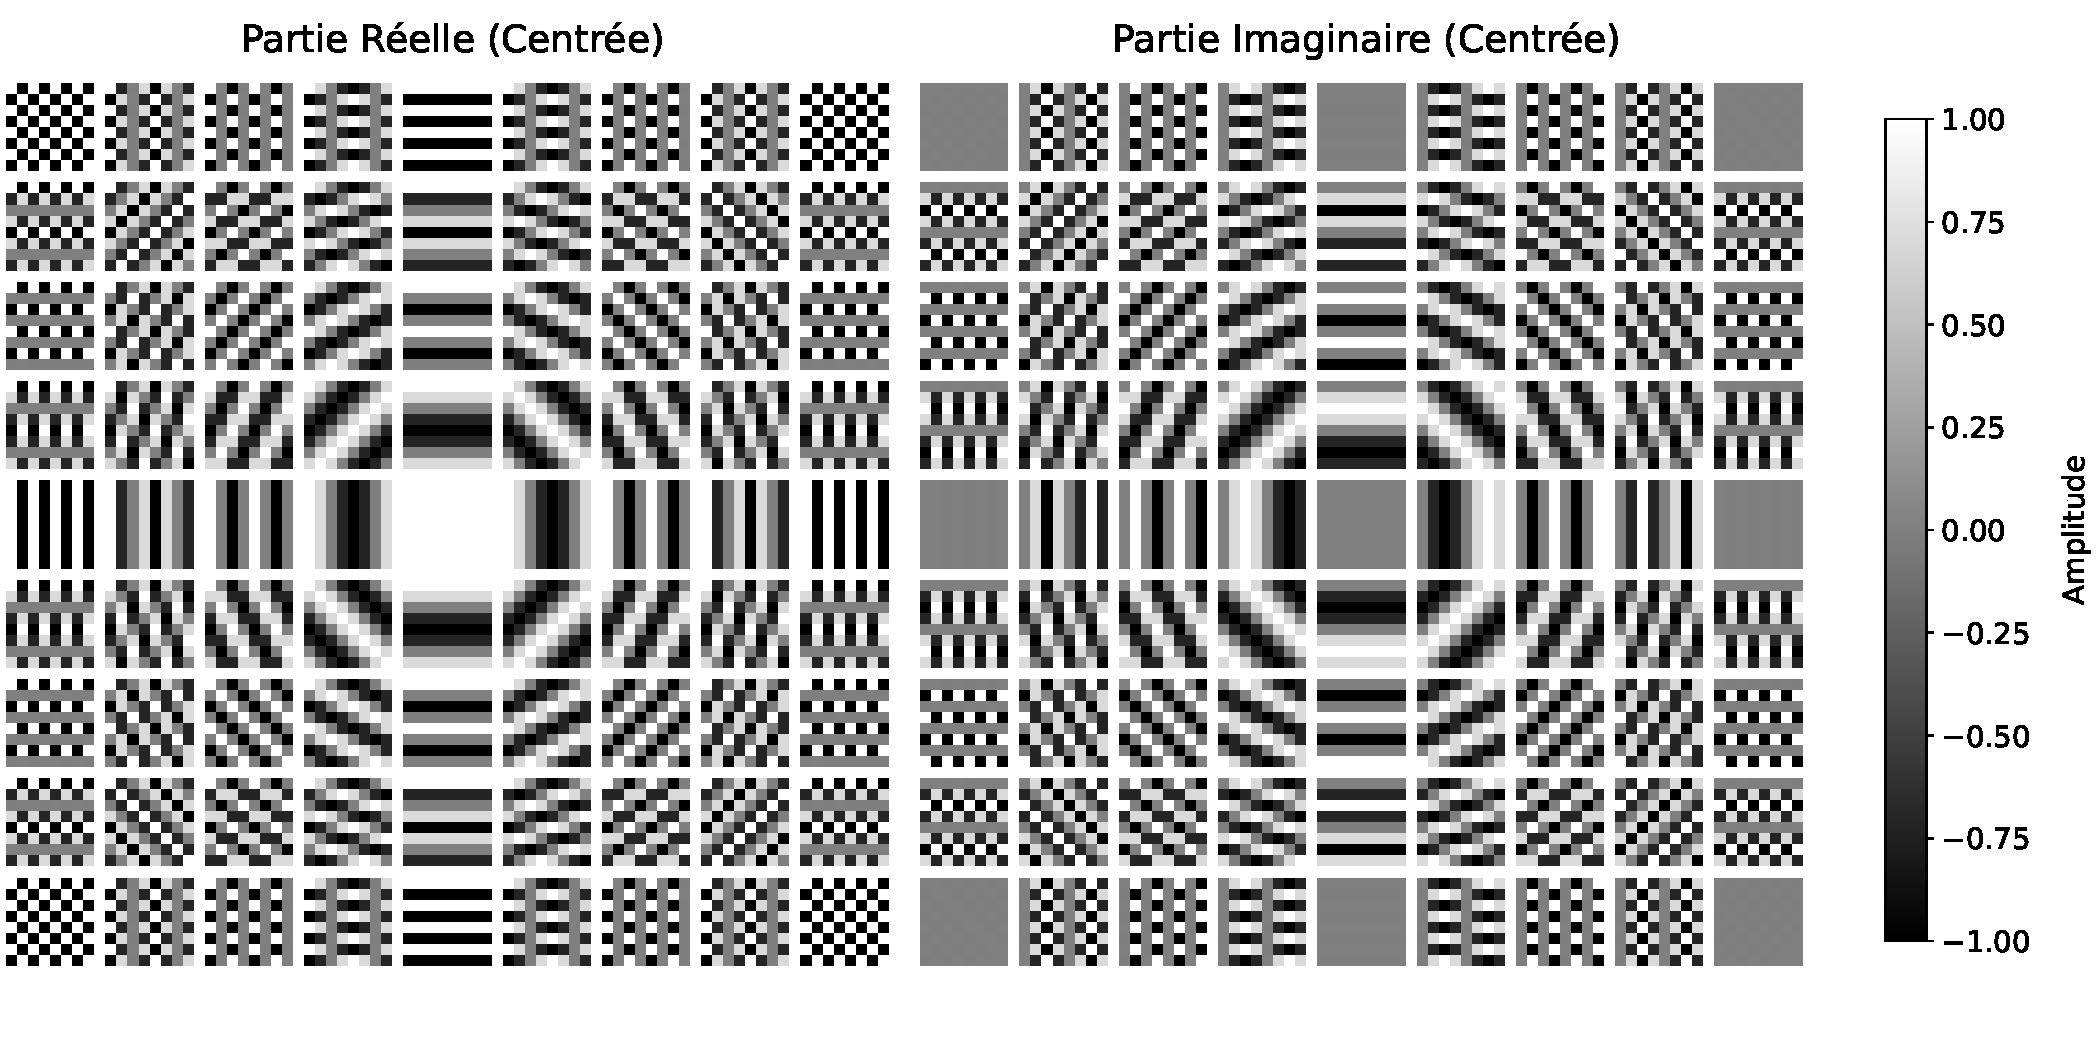
\includegraphics[width=0.95\textwidth]{figures/theory/fourier_basis_2d.pdf}
    \caption{Visualisation des bases de Fourier 2D pour tous les couples de fréquences $(u,v)$ d'une image de taille $9 \times 9$. La partie réelle et la partie imaginaire sont affichées séparément. Les basses fréquences sont situées au centre des grilles, tandis que les hautes fréquences se trouvent en périphérie.}
    \label{fig:fourier_basis_2d}
\end{figure}

Dans les figures, on représentera parfois les fréquences de manière centrée, avec les basses fréquences
au centre de l'image. Cette convention est pratique pour la visualisation. En revanche, dans les formules,
les indices restent toujours dans $\{0,\dots,N-1\}$ et sont interprétés modulo $N$.

\subsection{Vectorisation et produit de Kronecker}

Dans tout le chapitre, nous vectorisons les images en empilant les colonnes. Pour
$X\in\mathbb{C}^{N\times N}$, on pose donc
\begin{equation}
\operatorname{vec}(X)
=
\begin{pmatrix}
X[0,0] \\
X[1,0] \\
\vdots \\
X[N-1,0] \\
X[0,1] \\
\vdots \\
X[N-1,N-1]
\end{pmatrix}.
\label{eq:def_vectorisation_colonnes}
\end{equation}
On lit d'abord la première colonne, puis la deuxième, et ainsi de suite. Avec cette convention,
l'entrée $X[m,n]$ correspond à l'indice vectorisé
\[
    m+Nn.
\]

Nous utiliserons aussi le produit de Kronecker, noté $\otimes$. Défini comme suit, soient
$A \in \mathbb{C}^{m \times n}$ et $B \in \mathbb{C}^{p \times q}$, alors la matrice par blocs de taille
$mp \times nq$ est définie par

$$
A \otimes B =
\begin{pmatrix}
a_{11}B & a_{12}B & \cdots & a_{1n}B \\
a_{21}B & a_{22}B & \cdots & a_{2n}B \\
\vdots  & \vdots  & \ddots & \vdots  \\
a_{m1}B & a_{m2}B & \cdots & a_{mn}B
\end{pmatrix}.
$$

Il permet notamment de construire
une base de Fourier 2D à partir de deux bases de Fourier 1D. Les propriétés algébriques de la
vectorisation et du produit de Kronecker sont déjà connues en analyse matricielle~\cite{horn2013matrix}.

Avec notre convention de vectorisation par colonnes, on a en particulier
\begin{equation}
    \operatorname{vec}(ab^T)
    =
    b\otimes a.
    \label{eq:vec_produit_exterieur}
\end{equation}

En appliquant cette identité à l'image de Fourier
\[
    \Phi_{u,v}=\phi_u\phi_v^T,
\]
on obtient
\begin{equation}
    \operatorname{vec}(\Phi_{u,v})
    =
    \phi_v\otimes\phi_u.
    \label{eq:vec_fourier_2d}
\end{equation}
Ainsi, dans toute la suite du chapitre, la colonne de $Q_N$ associée à la fréquence 2D $(u,v)$ sera notée
\[
    q_{u,v}
    =
    \phi_v\otimes\phi_u.
\]

On note alors
\begin{equation}
    Q_N = F_N \otimes F_N
    \label{eq:def_base_fourier_2d_vectorisee}
\end{equation}
la base de Fourier 2D vectorisée. Par unitarité de $F_N$ :
\[
    Q_N^H Q_N = I_{N^2}.
\]
Les colonnes de $Q_N$ forment donc une base orthonormée de $\mathbb{C}^{N^2}$.

Avec la notation précédente, la colonne associée à la fréquence $(u,v)$ est
\[
    (Q_N)_{w(u,v)}
    =
    q_{u,v}
    =
    \phi_v\otimes\phi_u.
\]
L'indice $w(u,v)$ est simplement l'indice aplati qui permet de passer du couple de fréquences
$(u,v)$ à un seul indice de colonne dans $Q_N$. Il est défini par
\begin{equation}
    w(u,v)=u+Nv.
    \label{eq:indice_frequence_aplati}
\end{equation}\

Réciproquement, si l'on connaît un indice aplati $w\in\{0,\dots,N^2-1\}$, on retrouve le couple
de fréquences correspondant par
\[
    u = w \bmod N,
    \qquad
    v = \left\lfloor \frac{w}{N} \right\rfloor.
\]

\section{Convolution discrète en dimension 1}

Avant d'étudier les images, nous commençons par le cas plus simple d'un signal discret périodique représenté 
par sa période $x = (x[0], x[1], \ldots, x[N-1])$ avec $x[i] \in \mathbb{R}$.
Soit $x \in \mathbb{R}^N$ notre signal et $h = (h[0], h[1], \ldots, h[N-1]) \in \mathbb{R}^N$ notre filtre (qui sera 
supposé de même taille que le signal, quitte à être complété par des zéros). 
La convolution circulaire entre $h$ et $x$ est définie par :

\[
y[n] = (h * x)[n] = \sum_{k=0}^{N-1} h[k]\,x[(n-k) \bmod N] \text{~\cite{ImagerieNumeriqueTheme7Block2}}
\]

L'opération modulo signifie que les indices du signal sont pris dans 
\(\mathbb{Z}_N\). 
Ainsi, lorsqu'un indice sort de l'intervalle \(\{0,\ldots,N-1\}\), 
il est ramené à sa classe correspondante dans \(\mathbb{Z}_N\).
Le signal est donc interprété comme périodique, comme l'illustre la 
figure~\ref{fig:padding_circulaire}. 

\begin{figure}[H]
    \centering
    \begin{tikzpicture}[
        node distance=0cm,
        cell/.style={rectangle, draw=black, thick, minimum width=1.2cm, minimum height=1.2cm, text centered, font=\large},
        pad/.style={rectangle, draw=gray, dashed, fill=gray!10, minimum width=1.2cm, minimum height=1.2cm, text centered, font=\large, text=gray}
    ]
    
    \node[cell] (x0) {$x_0$};
    \node[cell, right=of x0] (x1) {$x_1$};
    \node[cell, right=of x1] (x2) {$x_2$};
    \node[cell, right=of x2] (x3) {$x_3$};
    
    \node[pad, left=of x0] (pL1) {$x_3$};
    \node[pad, left=of pL1] (pL2) {$x_2$};
    
    \node[pad, right=of x3] (pR1) {$x_0$};
    \node[pad, right=of pR1] (pR2) {$x_1$};
    
    \draw [decorate,decoration={brace,amplitude=5pt,mirror}]
        (x0.south west) -- (x3.south east) node[midway,below=10pt] {Signal original $x$};
    
    \draw [decorate,decoration={brace,amplitude=5pt}, gray]
        (pL2.north west) -- (pL1.north east) node[midway,above=10pt] {\textit{Padding}};
        
    \draw [decorate,decoration={brace,amplitude=5pt}, gray]
        (pR1.north west) -- (pR2.north east) node[midway,above=10pt] {\textit{Padding}};

    \draw[->, thick, gray, dashed, bend left=45] (x3.north) to node[above] {} (pL1.north);
    \draw[->, thick, gray, dashed, bend right=45] (x0.south) to node[below] {} (pR1.south);

    \end{tikzpicture}
    \caption{Représentation du \textit{padding} circulaire pour un signal 1D. Les bords du signal se répètent de manière périodique.}
    \label{fig:padding_circulaire}
\end{figure}

\paragraph{Remarque sur l'hypothèse de périodicité.}

Dans cette section, nous travaillons avec des convolutions circulaires. Cela revient à considérer les
signaux comme périodiquement prolongés : lorsque l'on dépasse une extrémité du signal, on revient
de l'autre côté. Cette hypothèse est très utile mathématiquement, car elle permet de diagonaliser les
convolutions par la base de Fourier discrète.

Elle ne correspond cependant pas toujours au comportement exact des images réelles aux bords :
si les extrémités ne se raccordent pas naturellement, la périodisation peut créer une discontinuité
artificielle. Ce point est discuté plus en détail en annexe~\ref{app:periodicite-bords-gibbs}.

\section{Les fonctions de Fourier comme fonctions propres de la convolution circulaire}
\label{sec:fourier-vecteurs-propres}

\paragraph{Cas unidimensionnel}

On se place dans l'espace des signaux discrets périodiques de période $N$ :
\[
V_N = \{x : \mathbb{Z}_N \rightarrow \mathbb{C}\}.
\]
Un élément de $V_N$ peut être vu soit comme une fonction discrète périodique, soit comme un vecteur de $\mathbb{C}^N$.

Pour un filtre $h \in \mathbb{C}^N$ fixé, la convolution circulaire définit un opérateur linéaire
\[
\mathcal{C}_h : V_N \rightarrow V_N,
\qquad
\mathcal{C}_h(x) = h * x.
\]

Pour chaque fréquence $f \in \{0,\dots,N-1\}$, on utilise le vecteur de Fourier normalisé
$\phi_f$ défini en \eqref{eq:def_base_fourier_1d}.

Le résultat fondamental liant la convolution circulaire et la base de Fourier s'écrit alors :

\begin{equation}
\mathcal{C}_h(\phi_f) = \lambda_f \phi_f,
\label{eq:fourier_fonction_propre_conv_1d}
\end{equation}

c'est-à-dire, composante par composante :
\[
(h * \phi_f)[n] = \lambda_f \phi_f[n],
\]
où
\[
\lambda_f =
\sum_{k=0}^{N-1} h[k] e^{-2\mathrm{i}\pi f k/N}.
\]

Il est important de remarquer que $\lambda_f$ dépend du filtre $h$ et de la fréquence $f$,
mais pas de la position $n$. Ainsi, lorsque l'entrée de l'opérateur de convolution circulaire
est une onde de Fourier, la convolution ne modifie pas sa forme spatiale : elle se contente
de la multiplier par un scalaire complexe. Autrement dit, $\lambda_f$ est une valeur propre et
$\phi_f$ une fonction propre de l'opérateur de convolution circulaire
$\mathcal{C}_h$.

\begin{proof}
\begin{alignat*}{2}
    (\mathcal{C}_h(\phi_f))[n] &= (h * \phi_f)[n] \\
    &= \sum_{k=0}^{N-1} h[k]\,\phi_f[(n-k) \bmod N] \\
    \text{\small (périodicité de $\phi_f$)} \quad &= \sum_{k=0}^{N-1} h[k]\,\phi_f[n-k] \\
    \text{\small (propriété de l'exponentielle)} \quad &= \sum_{k=0}^{N-1} h[k] e^{-2\mathrm{i}\pi f k/N}\phi_f[n] \\
    &= \left(\sum_{k=0}^{N-1} h[k] e^{-2\mathrm{i}\pi f k/N}\right)\phi_f[n] \\
    &= \lambda_f \phi_f[n].
\end{alignat*}

\end{proof}

Ce résultat correspond au théorème de convolution discret : dans le domaine de Fourier,
une convolution circulaire devient une multiplication fréquence par fréquence. Ainsi,
lorsque l'entrée est une onde de Fourier pure \(\phi_f\), la convolution ne change pas
sa fréquence ; elle la multiplie seulement par un scalaire. On obtient donc \ref{eq:fourier_fonction_propre_conv_1d}

\subsection{Conséquence matricielle : diagonalisation des matrices circulantes}

Pour un filtre $h$ fixe, la convolution circulaire 1D définit une application linéaire de $\mathbb{C}^N \rightarrow \mathbb{C}^N$
car pour tous $x, y \in \mathbb{C}^N$ et tous $\alpha, \beta \in \mathbb{C}$ nous avons que
\begin{align*}
h * (\alpha x + \beta y) &= \alpha (h * x) + \beta (h * y)
\end{align*}

\begin{proof}
\begin{alignat*}{2}
    (h * (\alpha x + \beta y))[n] &= \sum_{k=0}^{N-1} h[k]\,(\alpha x + \beta y)[(n-k) \bmod N]  \\
    &= \sum_{k=0}^{N-1} h[k]\,(\alpha x[(n-k) \bmod N] + \beta y[(n-k) \bmod N])  \\
    &= \alpha \sum_{k=0}^{N-1} h[k]\,x[(n-k) \bmod N] + \beta \sum_{k=0}^{N-1} h[k]\,y[(n-k) \bmod N]  \\
    &= \alpha (h * x)[n] + \beta (h * y)[n].
\end{alignat*}

\end{proof}

Comme cette opération est linéaire, le rappel de l'annexe~\ref{app:representation-lineaire-matrice}
garantit qu'elle peut être représentée, une fois une base choisie, par une matrice
$C_h \in \mathbb{C}^{N \times N}$ telle que pour tout signal d'entrée $x \in \mathbb{C}^N$ :

$$
y = C_h x.
$$

où $C_h$ est une matrice circulante construite à partir du filtre $h$ telle que la première ligne est organisée de manière à reproduire $y[0]$,
puis chaque ligne suivante est obtenue par décalage circulaire :

$$
C_h =
\begin{pmatrix}
h[0] & h[N-1] & h[N-2] & \cdots & h[1] \\
h[1] & h[0] & h[N-1] & \cdots & h[2] \\
h[2] & h[1] & h[0] & \cdots & h[3] \\
\vdots & \vdots & \vdots & \ddots & \vdots \\
h[N-1] & h[N-2] & h[N-3] & \cdots & h[0]
\end{pmatrix}.
$$

En effet, $y[0] = h[0]x[0] + h[1]x[N-1] + \cdots + h[N-1]x[1]$ correspond à la première ligne de $C_h$ 
multipliée par le vecteur $x$, en appliquant itérativement la même logique on obtient les autres éléments de $y$.

\vspace{0.5cm}

En choisissant la base canonique de $\mathbb{C}^N$, l'opérateur linéaire $\mathcal{C}_h$
est représenté par la matrice circulante $C_h$. La relation
$\mathcal{C}_h(\phi_f) = \lambda_f \phi_f$ peut alors être réécrite sous forme matricielle :

\begin{equation}
    C_h \phi_f = \lambda_f \phi_f
    \label{eq:fourier_eigen_matrice}
\end{equation}

Ainsi, chaque fonction de Fourier $\phi_f$ est un vecteur propre de la matrice circulante $C_h$,
avec valeur propre associée $\lambda_f$. Ce qui signifie que dans le cadre 
circulaire, la convolution agit diagonalement dans la base de Fourier.

En utilisant la matrice de Fourier $F_N$ définie en \eqref{eq:def_matrice_fourier_1d},
on regroupe les valeurs propres dans la matrice diagonale :
$$
\Lambda_h =
\operatorname{diag}(\lambda_0,\lambda_1,\ldots,\lambda_{N-1}).
$$

L'égalité vectorielle \eqref{eq:fourier_eigen_matrice} pour toutes les fréquences devient :

\begin{align}
C_h F_N &= F_N \Lambda_h \notag \\
\text{(par unitarité de \(F_N\))}\qquad
\Longleftrightarrow\quad
C_h &= F_N \Lambda_h F_N^H.
\end{align}

\section{Convolution circulaire en dimension 2}
\label{sec:convolution-circulaire-2d}

Nous étendons maintenant le résultat précédent au cas des images carrées. Soit
$X\in\mathbb{C}^{N\times N}$ une image et soit
$h\in\mathbb{C}^{N\times N}$ un filtre. La convolution circulaire 2D est définie par
\begin{equation}
    Y[m,n]
    =
    (h * X)[m,n]
    =
    \sum_{a=0}^{N-1}
    \sum_{b=0}^{N-1}
    h[a,b]\,
    X[(m-a)\bmod N,\,(n-b)\bmod N].
    \label{eq:def_convolution_circulaire_2d}
\end{equation}

Nous utilisons les images de Fourier 2D définies en \eqref{eq:def_base_fourier_2d} :
\[
    \Phi_{u,v}[m,n]
    =
    \phi_u[m]\phi_v[n].
\]
Comme en dimension 1, un décalage circulaire d'une base de Fourier ne change pas sa forme, mais la
multiplie par un facteur complexe :
\[
    \phi_u[(m-a)\bmod N]
    =
    e^{-2\pi iua/N}\phi_u[m],
    \qquad
    \phi_v[(n-b)\bmod N]
    =
    e^{-2\pi ivb/N}\phi_v[n].
\]
Ainsi,
\[
    \Phi_{u,v}[(m-a)\bmod N,(n-b)\bmod N]
    =
    e^{-2\pi i(ua+vb)/N}
    \Phi_{u,v}[m,n],
\]

ou $(ua + vb) \in \mathbb{Z}_N$.

En appliquant la convolution circulaire 2D à $\Phi_{u,v}$, on obtient
\begin{align}
(h * \Phi_{u,v})[m,n]
&=
\sum_{a=0}^{N-1}
\sum_{b=0}^{N-1}
h[a,b]\,
\Phi_{u,v}[(m-a)\bmod N,(n-b)\bmod N]
\nonumber \\
&=
\left(
\sum_{a=0}^{N-1}
\sum_{b=0}^{N-1}
h[a,b]e^{-2\pi i(ua+vb)/N}
\right)
\Phi_{u,v}[m,n].
\end{align}

On définit donc
\begin{equation}
    \lambda_{u,v}
    =
    \sum_{a=0}^{N-1}
    \sum_{b=0}^{N-1}
    h[a,b]e^{-2\pi i(ua+vb)/N}.
    \label{eq:valeur_propre_convolution_2d}
\end{equation}
On obtient finalement
\begin{equation}
    h * \Phi_{u,v}
    =
    \lambda_{u,v}\Phi_{u,v}.
    \label{eq:fourier_fonction_propre_conv_2d}
\end{equation}

\section{Représentation matricielle d'une convolution 2D}

Nous utilisons maintenant la vectorisation par colonnes définie en
\eqref{eq:def_vectorisation_colonnes}. Comme la convolution circulaire est linéaire, il existe
une matrice
\[
    M \in \mathbb{C}^{N^2\times N^2}
\]
telle que
\begin{equation}
    \operatorname{vec}(Y)
    =
    M\operatorname{vec}(X).
\end{equation}

Autrement dit, le coefficient de $M$ situé à la ligne $m+Nn$ et à la colonne $r+Ns$ indique comment le pixel
$X[r,s]$ contribue au pixel $Y[m,n]$.

La matrice $M$ en question applique le filtre $h$ sur chaque pixel de notre image $X$ en une seule opération.
À cette fin, la matrice $M$ possède une structure bloc-circulante à blocs circulants (BCCB)
comme illustré ci-dessous :

\begin{figure}[H]
\centering

\begin{tikzpicture}[
    scale=0.75, transform shape, % Réduction globale équilibrée
    font=\small,
    block/.style={
        draw=black!65,
        rounded corners=1pt,
        minimum width=1.0cm,  % Réduit de 1.25
        minimum height=0.55cm, % Réduit de 0.70
        inner sep=1pt,
        fill=gray!6,
        align=center
    },
    diagblock/.style={
        block,
        fill=gray!18,
        draw=black!85,
        line width=0.5pt
    },
    frame/.style={
        draw=black!85,
        rounded corners=2pt,
        line width=0.6pt
    },
    arrow/.style={
        -{Stealth[length=1.5mm]},
        semithick,
        black!65
    }
]

% --- Matrice M (plus compacte) ---
\matrix (B) [
    matrix of nodes,
    nodes={block},
    row sep=1.5pt,    % Espacement réduit
    column sep=1.5pt  % Espacement réduit
] {
|[diagblock]|$C_0$     & $C_{N-1}$ & $\cdots$ & $C_2$     & $C_1$     \\
$C_1$                 & |[diagblock]|$C_0$ & $\cdots$ & $C_3$     & $C_2$     \\
$\vdots$              & $\vdots$   & $\ddots$ & $\vdots$  & $\vdots$  \\
$C_{N-2}$             & $C_{N-3}$  & $\cdots$ & |[diagblock]|$C_0$ & $C_{N-1}$ \\
$C_{N-1}$             & $C_{N-2}$  & $\cdots$ & $C_1$     & |[diagblock]|$C_0$ \\
};

\node[frame, fit=(B-1-1)(B-5-5), inner sep=3pt] (bigmatrix) {};

% Titre compact avec sous-titre intégré
\node[above=2pt of bigmatrix, align=center] {
    \textbf{\(M \in\mathbb{C}^{N^2\times N^2}\)} \\ 
    \scriptsize (Bloc-circulante : décalage par blocs)
};

% --- Flèche de zoom plus courte ---
\draw[arrow] (bigmatrix.east) -- ++(0.7,0) node[midway, above, font=\tiny] {zoom};

% --- Bloc Ck (Matrice resserrée) ---
\node[anchor=west] (circulant) at ($(bigmatrix.east)+(0.9cm,0)$) {$\displaystyle
C_k =
\begin{bmatrix}
h_{0,k}     & \cdots & h_{1,k} \\
h_{1,k}     & \cdots & h_{2,k} \\
\vdots      & \ddots & \vdots  \\
h_{N-1,k}   & \cdots & h_{0,k}
\end{bmatrix}
$};

\node[frame, fit=(circulant), inner sep=2pt] (smallmatrix) {};

% Titre compact pour Ck
\node[above=2pt of smallmatrix, align=center] {
    \textbf{Bloc \(C_k\) circulant} \\
    \scriptsize (décalage interne)
};

\end{tikzpicture}

\caption{Structure compacte d'une matrice BCCB (doublement circulante).}
\label{fig:bccb-structure}
\end{figure}

On dit alors que $M$ est une matrice \textbf{BCCB} (\textit{Block-Circulant with Circulant Blocks}~\cite{jain1989fundamentals}).
Le détail est donné en annexe~\ref{app:preuve_bccb}.

Le résultat spectral obtenu pour la convolution circulaire 2D s'écrit alors, sous forme vectorisée,
\[
    M\operatorname{vec}(\Phi_{u,v})
    =
    \lambda_{u,v}\operatorname{vec}(\Phi_{u,v}).
\]

\subsection{Diagonalisation par le produit de Kronecker des bases de Fourier}

D'après le résultat précédent \ref{eq:fourier_fonction_propre_conv_2d} comme \(q_{u,v}=\operatorname{vec}(\Phi_{u,v})\), on obtient
\[
    M q_{u,v}
    =
    \lambda_{u,v} q_{u,v}.
\]
l'égalité matricielle pour toutes les fréquences devient
\begin{equation}
    \begin{split}
        M Q_N &= Q_N \Lambda_h \\
        \Longleftrightarrow \text{\footnotesize (unitarité de $Q_N$)} \quad M &= Q_N \Lambda_h Q_N^H.
    \end{split}
    \label{eq:diagonalisation_conv_2d}
\end{equation}
où $\Lambda_h$ est la matrice diagonale contenant les valeurs propres $\lambda_{u,v}$
dans le même ordre que les colonnes $q_{u,v}$ de $Q_N$.

\section{Extension au cas multi-canaux}

Jusqu'ici, nous avons considéré le cas d'une convolution mono-canal, c'est-à-dire que les images 
d'entrée et de sortie sont constituées d'un seul canal (par exemple, une image en niveaux de gris). 
Maintenant, nous allons considérer le cas plus général d'une convolution multi-canaux :
\[
    X \in\mathbb{C}^{m_{in} \times N \times N}, \qquad Y \in\mathbb{C}^{m_{out} \times N \times N},
\]
où $m_{in}$ et $m_{out}$ désignent le nombre de canaux d'entrée et de sortie respectivement.

Ainsi, pour chaque canal de sortie $Y_i$, nous avons que :
\begin{equation}
    Y_i = \sum_{j=1}^{m_{in}} h_{i,j} * X_j \qquad\text{pour } i=1,\dots,m_{out},
    \label{eq:conv_multi}
\end{equation}
où $h_{i,j}$ est le filtre de convolution appliqué au canal d'entrée $j$ pour produire le canal de sortie $i$.

% \begin{figure}[H]
%     \centering
%     % J'ai baissé très légèrement le scale à 0.85 pour que ce schéma plus large rentre 
%     % parfaitement dans les marges classiques d'un document A4.
%     \begin{tikzpicture}[>=stealth, font=\sffamily, scale=0.85, every node/.style={transform shape}]
        
%         % ==========================================
%         % Couleurs
%         % ==========================================
%         \definecolor{gridblue}{HTML}{006699}
%         \definecolor{gridred}{HTML}{E74C3C}
%         \definecolor{gridteal}{HTML}{148F77}
%         \definecolor{gridorange}{HTML}{F39C12}
%         \definecolor{bglight}{HTML}{F8F9FA}

%         % ==========================================
%         % Zones de fond (Structuration élargie)
%         % ==========================================
%         \draw[fill=bglight, draw=gray!40, dashed, rounded corners=5pt] 
%             (-1.0, -1.0) rectangle (1.0, 6.0);
%         \node[gray, font=\bfseries\small] at (0, 5.65) {Entrée $X$};

%         \draw[fill=bglight, draw=gray!40, dashed, rounded corners=5pt] 
%             (3.0, -1.0) rectangle (5.0, 6.0);
%         \node[gray, font=\bfseries\small, align=center] at (4.0, 5.65) {Filtres $h_i$};

%         \draw[fill=bglight, draw=gray!40, dashed, rounded corners=5pt] 
%             (7.0, -1.0) rectangle (9.0, 6.0);
%         \node[gray, font=\bfseries\small, align=center] at (8.0, 5.65) {Cartes $Z_i$};

%         \draw[fill=bglight, draw=gray!40, dashed, rounded corners=5pt] 
%             (10.8, -1.0) rectangle (15.5, 6.0);
%         \node[gray, font=\bfseries\small, align=center] at (13.15, 5.65) {Somme et Sortie};

%         % ==========================================
%         % 1. Canal Supérieur (m_in)
%         % ==========================================
%         % X_min (Centre x=0, y=3.8)
%         \filldraw[fill=gridblue!10, draw=gridblue, thick] 
%             (-0.625, 3.175) rectangle ++(1.25,1.25);
%         \draw[gridblue!40, step=0.3125] (-0.625, 3.175) grid ++(1.25,1.25);
%         \node[gridblue, font=\bfseries\scriptsize, fill=white, fill opacity=0.8, text opacity=1, inner sep=1.5pt] 
%             at (0, 3.8) {$X_{m_{\mathrm{in}}}$};

%         % Conv node * (Centre x=4.0, y=3.8)
%         \node[circle, draw=gridorange, fill=gridorange!10, thick, minimum size=0.5cm, inner sep=0pt] 
%             (convtop) at (4.0, 3.8) {$*$};

%         % h_min (Centre x=4.0, y=5.0)
%         \filldraw[fill=gridred!10, draw=gridred, thick] 
%             (3.575, 4.575) rectangle ++(0.85,0.85);
%         \draw[gridred!45, step=0.2125] (3.575, 4.575) grid ++(0.85,0.85);
%         \node[gridred, font=\bfseries\scriptsize, fill=white, fill opacity=0.8, text opacity=1, inner sep=1.5pt] 
%             at (4.0, 5.0) {$h_{i,m_{\mathrm{in}}}$};

%         % Z_min (Centre x=8.0, y=3.8)
%         \filldraw[fill=gridorange!15, draw=gridorange, thick] 
%             (7.45, 3.25) rectangle ++(1.10,1.10);
%         \draw[gridorange!45, step=0.275] (7.45, 3.25) grid ++(1.10,1.10);
%         \node[gridorange!80!black, font=\bfseries\scriptsize, fill=white, fill opacity=0.8, text opacity=1, inner sep=1.5pt] 
%             at (8.0, 3.8) {$Z_{i,m_{\mathrm{in}}}$};

%         % Flèches Canal m_in
%         \draw[->, thick, gridblue] (0.625, 3.8) -- (convtop.west);
%         \draw[->, thick, gridred] (4.0, 4.575) -- (convtop.north);
%         \draw[->, thick, gridorange] (convtop.east) -- (7.45, 3.8);

%         % ==========================================
%         % 2. Canal Inférieur (1)
%         % ==========================================
%         % X_1 (Centre x=0, y=0)
%         \filldraw[fill=gridblue!25, draw=gridblue, thick] 
%             (-0.625, -0.625) rectangle ++(1.25,1.25);
%         \draw[gridblue!45, step=0.3125] (-0.625, -0.625) grid ++(1.25,1.25);
%         \node[gridblue, font=\bfseries\scriptsize, fill=white, fill opacity=0.85, text opacity=1, inner sep=2pt] 
%             at (0, 0) {$X_1$};

%         % Conv node * (Centre x=4.0, y=0)
%         \node[circle, draw=gridorange, fill=gridorange!10, thick, minimum size=0.5cm, inner sep=0pt] 
%             (convbot) at (4.0, 0) {$*$};

%         % h_1 (Centre x=4.0, y=1.2)
%         \filldraw[fill=gridred!25, draw=gridred, thick] 
%             (3.575, 0.775) rectangle ++(0.85,0.85);
%         \draw[gridred!45, step=0.2125] (3.575, 0.775) grid ++(0.85,0.85);
%         \node[gridred, font=\bfseries\scriptsize, fill=white, fill opacity=0.85, text opacity=1, inner sep=2pt] 
%             at (4.0, 1.2) {$h_{i,1}$};

%         % Z_1 (Centre x=8.0, y=0)
%         \filldraw[fill=gridorange!25, draw=gridorange, thick] 
%             (7.45, -0.55) rectangle ++(1.10,1.10);
%         \draw[gridorange!45, step=0.275] (7.45, -0.55) grid ++(1.10,1.10);
%         \node[gridorange!80!black, font=\bfseries\scriptsize, fill=white, fill opacity=0.85, text opacity=1, inner sep=2pt] 
%             at (8.0, 0) {$Z_{i,1}$};

%         % Flèches Canal 1
%         \draw[->, thick, gridblue] (0.625, 0) -- (convbot.west);
%         \draw[->, thick, gridred] (4.0, 0.775) -- (convbot.north);
%         \draw[->, thick, gridorange] (convbot.east) -- (7.45, 0);

%         % ==========================================
%         % 3. Intermédiaires (Points de suspension)
%         % ==========================================
%         \node[gridblue, font=\Large] at (0, 1.9) {$\vdots$};
%         \node[gridorange, font=\Large] at (4.0, 1.9) {$\vdots$}; 
%         \node[gridorange!80!black, font=\Large] at (8.0, 1.9) {$\vdots$};

%         % ==========================================
%         % 4. Somme & Sortie
%         % ==========================================
%         % Sum (Centre x=12.0)
%         \node[circle, draw=gridteal, fill=gridteal!10, thick, minimum size=0.85cm] 
%             (sum) at (12.0, 1.9) {\Large $\sum$};
%         \node[gridteal, font=\scriptsize, align=center] at (12.0, 1.1) {somme\\sur $j$};

%         % Flèches Z -> Somme
%         \draw[->, thick, gridorange] (8.55, 3.8) to[out=0,in=135] (sum.north west);
%         \draw[->, thick, gridorange] (8.55, 0) to[out=0,in=225] (sum.south west);

%         % Y_i (Centre x=14.2)
%         \filldraw[fill=gridteal!22, draw=gridteal, thick] 
%             (13.525, 1.225) rectangle ++(1.35,1.35);
%         \draw[gridteal!45, step=0.3375] (13.525, 1.225) grid ++(1.35,1.35);
%         \node[gridteal, font=\bfseries\scriptsize, fill=white, fill opacity=0.85, text opacity=1, inner sep=2pt] 
%             at (14.2, 1.9) {$Y_i$};

%         % Flèche Somme -> Y_i
%         \draw[->, thick, gridteal] (sum.east) -- (13.525, 1.9);

%         % ==========================================
%         % 5. Equations Mathématiques (En bas, aérées)
%         % ==========================================
%         \node[gridblue, font=\bfseries\small] at (0, -1.8) {$X \in \mathbb{C}^{m_{\mathrm{in}}\times N\times N}$};
%         \node[gridred, font=\bfseries\small] at (4.0, -1.8) {$h_i \in \mathbb{C}^{m_{\mathrm{in}}\times k\times k}$};
%         \node[gridorange!80!black, font=\bfseries\small] at (8.0, -1.8) {$Z_{i,j}=h_{i,j} * X_j$};
%         \node[gridteal, font=\bfseries\small] at (13.15, -1.8) {$Y_i=\displaystyle\sum_{j=1}^{m_{\mathrm{in}}} Z_{i,j}$};

%     \end{tikzpicture}

%     \vspace{0.3cm}
%     \caption{
%     Convolution multi-canaux produisant un canal de sortie $Y_i$.
%     }
%     \label{fig:conv_multi_canaux}
% \end{figure}

\subsection{Mélange des canaux à fréquence fixée}
\label{subsec:melange_canaux_frequence_fixee}

Soit une fréquence spatiale $(u,v)$ et l'image de Fourier correspondante $\Phi_{u,v}$.
On suppose que chaque canal d'entrée contient cette même fréquence spatiale, mais avec une amplitude
différente :
\[
    X_j = \alpha_j \Phi_{u,v},
    \qquad j=1,\dots,m_{\mathrm{in}}.
\]
Le vecteur
\[
    \alpha = (\alpha_1,\dots,\alpha_{m_{\mathrm{in}}})^T
\]
contient donc les amplitudes de cette fréquence dans les différents canaux d'entrée.

En injectant ces entrées dans \eqref{eq:conv_multi} et par linéarité de la convolution, on obtient, pour le canal de sortie $i$,
\begin{align*}
Y_i
&=
\sum_{j=1}^{m_{\mathrm{in}}} h_{i,j} * X_j \\
&=
\sum_{j=1}^{m_{\mathrm{in}}} \alpha_j (h_{i,j} * \Phi_{u,v}) \\
&=
\sum_{j=1}^{m_{\mathrm{in}}} \alpha_j \lambda^{i,j}_{u,v}\Phi_{u,v} \\
&=
\left(
    \sum_{j=1}^{m_{\mathrm{in}}}
    \lambda^{i,j}_{u,v}\alpha_j
\right)
\Phi_{u,v}.
\end{align*}

On introduit alors la matrice de mélange associée à la fréquence $(u,v)$ :
\[
    G^{(u,v)} \in \mathbb{C}^{m_{\mathrm{out}}\times m_{\mathrm{in}}},
    \qquad
    G^{(u,v)}_{i,j}
    =
    \lambda^{i,j}_{u,v}.
\]
Si $\beta\in\mathbb{C}^{m_{\mathrm{out}}}$ désigne les amplitudes de sortie de cette même fréquence,
on peut écrire simplement
\[
    \beta = G^{(u,v)}\alpha.
\]

Cette écriture résume le rôle d'une convolution multi-canaux : pour une fréquence spatiale fixée,
elle effectue un mélange linéaire entre les canaux. 

\subsection{Forme matricielle globale}

Pour écrire l'opération multi-canaux sous forme matricielle globale, on définit :
\[
\mathbf{x}
=
\begin{pmatrix}
\operatorname{vec}(X_1) \\
\vdots \\
\operatorname{vec}(X_{m_{\mathrm{in}}})
\end{pmatrix}
\in \mathbb{C}^{m_{\mathrm{in}}N^2},
\qquad
\mathbf{y}
=
\begin{pmatrix}
\operatorname{vec}(Y_1) \\
\vdots \\
\operatorname{vec}(Y_{m_{\mathrm{out}}})
\end{pmatrix}
\in \mathbb{C}^{m_{\mathrm{out}}N^2}.
\]

Pour chaque paire de canaux $(i,j)$, on note $B^{i,j}$ la matrice de convolution spatiale
associée au filtre $h_{i,j}$, c'est-à-dire la matrice qui applique la convolution entre le canal
d'entrée $j$ et le canal de sortie $i$.
On utilise la base de Fourier 2D vectorisée $Q_N$ définie en
\eqref{eq:def_base_fourier_2d_vectorisee}. Pour chaque paire de canaux $(i,j)$, la matrice
$B^{i,j}$ se diagonalise donc sous la forme
\[
    B^{i,j}
    =
    Q_N D^{i,j} Q_N^H,
\]
où
\[
D^{i,j}
=
\operatorname{diag}\bigl(
\lambda^{i,j}_{u,v}
\bigr)_{(u,v)\in\{0,\dots,N-1\}^2}.
\]

Les coefficients diagonaux de $D^{i,j}$ sont ordonnés selon l'indice aplati
$w(u,v)$ défini en \eqref{eq:indice_frequence_aplati}.

À présent nous pouvons introduire la matrice globale $M \in \mathbb{C}^{m_{out}N^2 \times m_{in}N^2}$
qui représente la couche de convolution complète sous la forme d'une matrice par blocs de taille
$m_{out} \times m_{in}$, où chaque bloc $(i,j)$ correspond à l'application du filtre $h_{i,j}$ :

$$
M =
\begin{pmatrix}
B^{1,1} & \cdots & B^{1,m_{in}} \\
\vdots & \ddots & \vdots \\
B^{m_{out},1} & \cdots & B^{m_{out},m_{in}}
\end{pmatrix}.
$$

Comme la même base $Q_N$ diagonalise tous les blocs spatiaux $B^{i,j}$, on peut factoriser le changement
de base spatial de part et d'autre de la matrice par blocs. On obtient alors

\begin{equation}
    M = (I_{m_{out}} \otimes Q_N) L (I_{m_{in}} \otimes Q_N)^H
    \label{eq:factorisation_M}
\end{equation}

où $L \in \mathbb{C}^{m_{out}N^2 \times m_{in}N^2}$ est une matrice composée de blocs diagonaux :

$$
L =
\begin{pmatrix}
D^{1,1} & \cdots & D^{1,m_{in}} \\
\vdots & \ddots & \vdots \\
D^{m_{out},1} & \cdots & D^{m_{out},m_{in}}
\end{pmatrix}.
$$

\vspace{0.5cm}
\begin{proof}

Par définition du produit de Kronecker, les opérations 
$I_{m_{out}} \otimes Q_N$ et $(I_{m_{in}} \otimes Q_N)^H = I_{m_{in}} \otimes Q_N^H$ 
génèrent des matrices diagonales par blocs :

$$
I_{m_{out}} \otimes Q_N = 
\begin{pmatrix}
Q_N & 0 & \cdots & 0 \\
0 & Q_N & \cdots & 0 \\
\vdots & \vdots & \ddots & \vdots \\
0 & 0 & \cdots & Q_N
\end{pmatrix},
\quad
I_{m_{in}} \otimes Q_N^H = 
\begin{pmatrix}
Q_N^H & 0 & \cdots & 0 \\
0 & Q_N^H & \cdots & 0 \\
\vdots & \vdots & \ddots & \vdots \\
0 & 0 & \cdots & Q_N^H
\end{pmatrix}.
$$

En calculant le produit matriciel par blocs à gauche, $Q_N$ se distribue sur chaque bloc des lignes 
correspondantes de $L$ :

$$
(I_{m_{out}} \otimes Q_N) L = 
\begin{pmatrix}
Q_N D^{1,1} & \cdots & Q_N D^{1,m_{in}} \\
\vdots & \ddots & \vdots \\
Q_N D^{m_{out},1} & \cdots & Q_N D^{m_{out},m_{in}}
\end{pmatrix}.
$$

En multipliant ensuite ce résultat à droite par la seconde matrice diagonale par blocs, 
$Q_N^H$ se distribue sur chaque bloc des colonnes correspondantes :

$$
(I_{m_{out}} \otimes Q_N) L (I_{m_{in}} \otimes Q_N)^H = 
\begin{pmatrix}
Q_N D^{1,1} Q_N^H & \cdots & Q_N D^{1,m_{in}} Q_N^H \\
\vdots & \ddots & \vdots \\
Q_N D^{m_{out},1} Q_N^H & \cdots & Q_N D^{m_{out},m_{in}} Q_N^H
\end{pmatrix}.
$$

Puisque la décomposition de la convolution mono-canal donne $B^{i,j} = Q_N D^{i,j} Q_N^H$ pour 
tout couple $(i,j)$, on obtient :

$$
(I_{m_{out}} \otimes Q_N) L (I_{m_{in}} \otimes Q_N)^H = 
\begin{pmatrix}
B^{1,1} & \cdots & B^{1,m_{in}} \\
\vdots & \ddots & \vdots \\
B^{m_{out},1} & \cdots & B^{m_{out},m_{in}}
\end{pmatrix}
= M.
$$
\end{proof}

On retrouve ainsi la forme de la \textbf{Proposition 1} de l'article de Tsuzuku et Sato~\cite{tsuzuku2019structural}. 
Elle sépare deux phénomènes :
\begin{itemize}
    \item les matrices $(I\otimes Q_N)$ réalisent le changement de base spatial vers le domaine de Fourier ;
    \item la matrice centrale $L$ contient les mélanges entre canaux, organisés fréquence par fréquence.
\end{itemize}

\section{Empilement linéaire de convolutions}
\label{sec:empilement-lineaire-convolutions}

Nous allons maintenant introduire la notion d'empilement de couches de convolution. 
L'idée est de modéliser mathématiquement le fonctionnement d'un réseau de neurones convolutifs profond, qui est 
composé de plusieurs couches appliquées successivement.

Comme nous l'avons vu dans les sections précédentes, notre cadre linéaire nous permet de représenter chaque couche 
de convolution de stride \(1\) (stride = pas voir \ref{fig:stride_comparison} pour une illustration) par une grande matrice globale \(M^{(k)}\). 
On note \(m_k\) le nombre de canaux en entrée de la couche \(k\), et \(m_{k+1}\) le nombre de canaux en sortie :
\[
M^{(k)} : \mathbb{C}^{m_k N^2} \longrightarrow \mathbb{C}^{m_{k+1}N^2}.
\]

Ainsi, pour une entrée vectorisée \(X \in \mathbb{C}^{m_1N^2}\), la sortie de la 
première couche s'écrit :
$$
X_1 = M^{(1)} X \in \mathbb{C}^{m_2 N^2}.
$$
En appliquant une seconde couche de convolution, on obtient :
$$
X_2 = M^{(2)} X_1 = M^{(2)}(M^{(1)} X) = (M^{(2)} M^{(1)}) X.
$$
En continuant ainsi pour $d$ couches de convolution successives :
\begin{equation}
M(X) = \left(M^{(d)} M^{(d-1)} \cdots M^{(1)}\right)X.
\label{eq:composition_couches}
\end{equation}

\subsection{Simplification par télescopage des transformations}

L'intérêt majeur de la décomposition matricielle de l'équation \eqref{eq:factorisation_M} réside 
dans son comportement lors du produit de plusieurs couches. Considérons deux couches 
successives $M^{(1)}$ et $M^{(2)}$. Leur produit s'écrit :
\begin{align*}
M^{(2)}M^{(1)} &= \left[ (I_{m_3} \otimes Q_N) L^{(2)} (I_{m_2} \otimes Q_N)^H \right] \left[ (I_{m_2} \otimes Q_N) L^{(1)} (I_{m_1} \otimes Q_N)^H \right] \\
&= (I_{m_3} \otimes Q_N) L^{(2)} \underbrace{\left( (I_{m_2} \otimes Q_N)^H (I_{m_2} \otimes Q_N) \right)}_{I_{m_2 N^2}} L^{(1)} (I_{m_1} \otimes Q_N)^H
\end{align*}

Par récurrence, pour un réseau de $d$ couches, la matrice globale $M$ se simplifie en :
\[
M = (I_{m_{d+1}} \otimes Q_N) L (I_{m_1} \otimes Q_N)^H
\]
où $L = L^{(d)} L^{(d-1)} \cdots L^{(1)}$ représente l'accumulation des mélanges de canaux.

\subsection{Indépendance fréquentielle et matrice de mélange $G^{(w)}$}

Comme chaque bloc interne des matrices $L^{(k)}$ est diagonal, le produit de ces matrices conserve cette structure.
En effet, le bloc $(i,j)$ du produit de deux matrices par blocs $L^{(2)}L^{(1)}$ s'écrit
\[
(L^{(2)}L^{(1)})_{i,j}
=
\sum_k D^{(2)}_{i,k}D^{(1)}_{k,j}.
\] 
Or le produit de deux matrices diagonales est diagonal, et une somme de matrices diagonales reste diagonale.
Par conséquent, chaque bloc de la matrice globale $L = L^{(d)}L^{(d-1)}\cdots L^{(1)}$ est encore une matrice diagonale de taille $N^2 \times N^2$.

Ainsi, dans un empilement linéaire de convolutions circulaires de stride $1$, la structure par fréquence
est conservée. Pour une fréquence donnée, seule la répartition entre les canaux évolue.

L'idée est alors la suivante : pour étudier ce que fait le réseau à une fréquence donnée, il n'est pas
nécessaire de regarder toute la grande matrice $L$. Il suffit de regarder, dans chaque bloc
$D^{(i,j)}$.

On regroupe ces coefficients dans une petite matrice
\[
    G^{(w)} \in \mathbb{C}^{m_{\mathrm{out}}\times m_{\mathrm{in}}},
\]
définie par
\begin{equation}
    \bigl(G^{(w)}\bigr)_{i,j}
    =
    \bigl(D^{(i,j)}\bigr)_{w,w}.
    \label{eq:def_matrice_frequence}
\end{equation}

La matrice $G^{(w)}$ décrit donc le comportement du réseau à la fréquence $w$. Elle ne décrit plus
toute l'image, mais seulement le mélange entre les canaux pour cette fréquence précise. C'est ce
qui permet de réduire l'étude d'une grande couche convolutionnelle à l'étude d'une matrice beaucoup
plus petite, fréquence par fréquence.

\subsection{Analyse de sensibilité par décomposition en valeurs singulières (SVD)}

L'opérateur de convolution multi-canaux peut être représenté par une matrice
\[
    M \in \mathbb{C}^{m_{\mathrm{out}}N^2 \times m_{\mathrm{in}}N^2}.
\]
Comme nous cherchons à identifier les directions d'entrée qui sont les plus amplifiées par la couche de 
convolution, il vient naturellement à l'esprit d'étudier les valeurs singulières de cette matrice.

La décomposition en valeurs singulières de $M$ s'écrit
\[
    M = U\Sigma V^H,
\]
où $U$ et $V$ sont des matrices unitaires, et où $\Sigma$ contient les valeurs singulières
\[
    \sigma_1 \geq \sigma_2 \geq \cdots \geq 0.
\]
Les colonnes de $V$ sont appelées vecteurs singuliers droits : elles correspondent aux directions
dans l'espace d'entrée. Les colonnes de $U$ sont les vecteurs singuliers gauches : elles correspondent
aux directions dans l'espace de sortie.

Une valeur singulière mesure l'amplification d'une direction d'entrée. Plus précisément, si $v_i$ est
un vecteur singulier droit associé à $\sigma_i$ et si $\|v_i\|_2=1$, alors
\[
    \|Mv_i\|_2 = \sigma_i.
\]
Ainsi, les grandes valeurs singulières correspondent aux directions d'entrée fortement amplifiées par
l'opérateur $M$. En particulier,
\[
\sigma_1(M)
= \max_{x \neq 0} \frac{\|Mx\|_2}{\|x\|_2}
= \max_{\|x\|_2 = 1} \|Mx\|_2
= \|M\|_2.
\]
La direction associée à $\sigma_1$ est donc une direction de sensibilité maximale, lorsque cette valeur
singulière est simple. Si elle est multiple, toute direction unitaire dans le sous-espace singulier associé
donne la même amplification.

Dans le cadre de notre analyse, les directions de forte sensibilité du réseau correspondent donc aux
vecteurs singuliers droits associés aux grandes valeurs singulières. Le lien détaillé entre SVD,
vecteurs propres de $M^H M$ et l'amplification est rappelé en annexe~\ref{app:svd-sensibilite}.

\subsection{Preuve de la structure du vecteur singulier de sensibilité}

\begin{proof}

Soit $\sigma$ une valeur singulière de la matrice de mélange
$G^{(w)}\in\mathbb{C}^{m_{\mathrm{out}}\times m_{\mathrm{in}}}$.
On note
\[
    a\in\mathbb{C}^{m_{\mathrm{in}}},
    \qquad
    b\in\mathbb{C}^{m_{\mathrm{out}}}
\]
les vecteurs singuliers droit et gauche associés. On a donc
\[
    G^{(w)}a=\sigma b,
    \qquad
    G^{(w)H}b=\sigma a.
\]

Dans l'espace complet du réseau, le vecteur singulier droit associé à cette fréquence $w$ s'écrit
\[
    v = (I_{m_1} \otimes Q_N) (a \otimes e_w),
\]
où $e_w$ est le vecteur de la base canonique, égal à $1$ à l'indice $w$ et à $0$ ailleurs.

On vérifie d'abord cette affirmation en appliquant l'opérateur $M$ à ce candidat $v$ :
\begin{align*}
M v &= \left[ (I_{m_{d+1}} \otimes Q_N) L (I_{m_1} \otimes Q_N)^H \right] \left[ (I_{m_1} \otimes Q_N) (a \otimes e_w) \right] \\
&= (I_{m_{d+1}} \otimes Q_N) L \underbrace{\left[ (I_{m_1} \otimes Q_N)^H (I_{m_1} \otimes Q_N) \right]}_{I_{m_1 N^2}} (a \otimes e_w) \\
M v &= (I_{m_{d+1}} \otimes Q_N) L (a \otimes e_w)
\end{align*}

Analysons maintenant l'action de $L$ sur le vecteur $(a \otimes e_w)$. Rappelons que $L$ est une matrice par blocs où 
chaque bloc $(i,j)$ est la matrice diagonale $D^{(i,j)}$. 
Le vecteur $(a \otimes e_w)$ peut être vu comme un vecteur par blocs dont le $j$-ième bloc est le vecteur $a_j e_w$. 
Ainsi, le $i$-ième bloc du vecteur résultant $y' = L (a \otimes e_w)$ se calcule par:
\[
y'_i = \sum_{j=1}^{m_1} D^{(i,j)} (a_j e_w)
\]

Puisque $D^{(i,j)}$ est une matrice diagonale, sa multiplication par le vecteur de la base canonique $e_w$ 
isole simplement son $w$-ième élément diagonal, multiplié par $e_w$. 
Autrement dit,

$$D^{(i,j)} e_w = (D^{(i,j)})_{w,w} \, e_w$$

Or, par définition de notre matrice de mélange fréquentiel, ce coefficient $(D^{(i,j)})_{w,w}$ est 
exactement l'élément $(i,j)$ de la matrice $G^{(w)}$. Nous obtenons donc directement :

$$y'_i = \sum_{j=1}^{m_1} (G^{(w)})_{i,j} \, a_j \, e_w = \left( \sum_{j=1}^{m_1} (G^{(w)})_{i,j} a_j \right) e_w$$

Le terme entre parenthèses n'est autre que la $i$-ième composante du produit matriciel $G^{(w)} a$. 
Sachant que $G^{(w)} a = \sigma b$, il vient :
\[
y'_i = (\sigma b)_i e_w = \sigma b_i e_w
\]

En réassemblant les blocs, nous déduisons que 
\begin{equation}
L(a \otimes e_w) = \sigma(b \otimes e_w).
\end{equation}
Nous pouvons maintenant réinjecter ce résultat dans notre équation :
\begin{align*}
M v &= (I_{m_{d+1}} \otimes Q_N) \left( \sigma (b \otimes e_w) \right) \\
&= \sigma \left( I_{m_{d+1}} b \otimes Q_N e_w \right) \\
M v &= \sigma \left( b \otimes (Q_N)_w \right)
\end{align*}

Cette équation montre que l'application de $M$ à $v$ produit bien un vecteur de la forme
\[
    Mv=\sigma u,
    \qquad
    u=b\otimes (Q_N)_w.
\]

Il reste à vérifier l'équation adjointe. Comme
\[
    u=(I_{m_{d+1}}\otimes Q_N)(b\otimes e_w),
\]
on obtient de la même manière
\[
    M^H u
    =
    (I_{m_1}\otimes Q_N)L^H(b\otimes e_w).
\]
Or la relation $G^{(w)H}b=\sigma a$ donne
\[
    L^H(b\otimes e_w)=\sigma(a\otimes e_w).
\]
Ainsi,
\[
    M^Hu
    =
    \sigma(a\otimes (Q_N)_w)
    =
    \sigma v.
\]
Les deux relations de la SVD sont donc vérifiées :
\[
    Mv=\sigma u,
    \qquad
    M^Hu=\sigma v.
\]

\end{proof}

\subsection{Vérification de l'orthonormalité :}

\begin{proof}

Pour que l'ensemble des vecteurs $v = a \otimes (Q_N)_w$ forme rigoureusement la matrice unitaire $V$ de la SVD de $M$, il doit constituer une base orthonormée. Cela se démontre grâce aux propriétés du produit scalaire mixte ($(A \otimes B)^H (C \otimes D) = (A^H C) \otimes (B^H D)$) :

\begin{itemize}
    \item \textbf{Norme unitaire :} Comme $a$ et $(Q_N)_w$ sont unitaires, $v^H v = (a^H a) \otimes ((Q_N)_w^H (Q_N)_w) = 1 \times 1 = 1$.
    \item \textbf{Orthogonalité intra-fréquentielle :} Pour une même fréquence $w$, l'orthogonalité native de deux vecteurs droits $a$ et $\tilde{a}$ est préservée : $v^H \tilde{v} = (a^H \tilde{a}) \otimes 1 = 0$.
    \item \textbf{Orthogonalité inter-fréquentielle :} Pour $w \neq \tilde{w}$, les colonnes de Fourier sont orthogonales : $v^H \tilde{v} = (a^H \tilde{a}) \otimes ((Q_N)_w^H (Q_N)_{\tilde{w}}) = 0$.

\end{itemize}

\end{proof}

\subsection{Expression finale du motif de Fourier}

Enfin, comme $Q_N e_w = (Q_N)_w$, l'expression du vecteur singulier devient
\[
    v
    =
    a \otimes (Q_N)_w.
\]
Si l'indice $w$ correspond au couple de fréquences $(u,v)$, alors, avec la notation $q_{u,v}$ fixée
dans la section~\ref{sec:conventions-fourier-vectorisation}, on peut écrire
\begin{equation}
    v
    =
    a \otimes q_{u,v}
    =
    a \otimes \bigl((F_N)_v \otimes (F_N)_u\bigr).
    \label{eq:vecteur_singulier_fourier_final}
\end{equation}

Autrement dit, le vecteur singulier est composé de deux parties : un vecteur $a$, qui décrit le
mélange entre les canaux, et une direction de Fourier $q_{u,v}$, qui décrit le motif spatial.

\section{Skip connections et couches de normalisation}
\label{sec:skip-normalisation}

Les résultats précédents ont été établis dans un cadre linéaire simplifié : les couches sont des convolutions
de stride $1$, sans activation non linéaire et avec un \textit{padding} circulaire. Dans ce cadre, nous avons montré que les directions de sensibilité maximale peuvent s'écrire sous la forme
d'un vecteur de canaux multiplié par une direction de Fourier spatiale, comme dans
\eqref{eq:vecteur_singulier_fourier_final}.

Il reste cependant à vérifier que cette conclusion ne disparaît pas dès que l'on ajoute deux mécanismes courants
des architectures convolutionnelles modernes : les \textit{skip connections} et les couches de normalisation. C'est
l'objet des Propositions 3 et 4 de Tsuzuku et Sato~\cite{tsuzuku2019structural}.

\subsection{Qu'est-ce qu'une \textit{skip connection} ?}

Les architectures convolutionnelles modernes, comme les réseaux résiduels (\textit{ResNet}) \cite{he2016deep}, 
utilisent fréquemment des \textit{skip connections}. 
Le principe consiste à ajouter directement l'entrée d'un bloc à sa sortie, de sorte que le bloc n'apprenne plus 
une transformation complète, mais une correction de l'identité.

Si l'on note $\mathcal{F}$ la transformation réalisée par le bloc, la sortie s'écrit
\begin{equation}
    x_{\ell+1} = \mathcal{F}(x_\ell) + x_\ell.
\end{equation}

Dans le cas simple où l'entrée et la sortie ont la même dimension, la branche de raccourci est donc l'identité. 
Dans le cadre de notre analyse linéaire, si l'on modélise le bloc principal par $M$, 
alors le bloc résiduel entier est représenté par
\begin{equation}
    M_{\mathrm{skip}} = M + I,
    \label{eq:skip_connection_matricielle}
\end{equation}
où $I$ désigne l'identité.

Cette écriture est particulièrement utile pour notre étude spectrale car elle montre que l'ajout d'une 
\textit{skip connection} ne change pas la nature de l'opérateur de base, mais ajoute simplement une contribution 
identité au bloc convolutionnel.

\begin{figure}[H]
\centering
\begin{tikzpicture}[
    >=Stealth,
    line/.style={->, semithick, black!85},
    branch/.style={semithick, black!85},
    font=\small,
    io/.style={inner sep=2pt, align=center},
    block/.style={
        draw=black!80,
        rounded corners=3pt,
        minimum width=2.8cm,
        minimum height=1.0cm,
        fill=gray!8,
        align=center
    },
    sum/.style={
        circle,
        draw=black!80,
        fill=gray!18,
        minimum size=7mm,
        inner sep=0pt,
        font=\normalsize\bfseries
    },
    lab/.style={font=\footnotesize, text=black!75}
]

% Noeuds principaux
\node[io] (x) at (0,0) {$x_\ell$};
\node[block] (M) at (3.1,0) {$M$};
\node[sum] (add) at (6.1,0) {$+$};
\node[io] (y) at (8.3,0) {$x_{\ell+1}$};

% Point de séparation
\coordinate (split) at (1.05,0);

% Coordonnées de la branche de raccourci
\coordinate (skipL) at (1.05,1.05);
\coordinate (skipR) at (6.1,1.05);

% Chemin principal
\draw[line] (x) -- (M);
\draw[line] (M) -- node[above, lab] {$Mx_\ell$} (add);
\draw[line] (add) -- node[above, lab] {$x_{\ell+1}$} (y);

% Marque du point de séparation
\fill[black!85] (split) circle (1.1pt);

% Branche de raccourci
\draw[branch] (split) -- (skipL);
\draw[branch] (skipL) -- node[above, lab] {$Ix_\ell = x_\ell$} (skipR);
\draw[line] (skipR) -- (add.north);

% Annotation sous le schéma
\node[lab] at (4.1,-0.95) {$x_{\ell+1}=Mx_\ell+x_\ell=(M+I)x_\ell$};

\end{tikzpicture}
\caption{Interprétation linéaire d'une \textit{skip connection}. Le chemin principal applique l'opérateur $M$, tandis que la branche de raccourci applique l'identité. Le bloc résiduel est donc représenté par l'opérateur $M+I$.}
\end{figure}

\subsection{Cas d'une skip connection}

\begin{proof}

Analysons d'abord le cas d'une connexion résiduelle "idéale", c'est-à-dire lorsque l'entrée $X$ et la sortie 
du bloc convolutionnel $M(X)$ \eqref{eq:composition_couches} possèdent exactement les mêmes dimensions (même résolution spatiale et même nombre 
de canaux). La transformation globale s'écrit alors tout simplement :
$$
M_{\mathrm{skip}}(X) = (M^{(d)} M^{(d-1)} \dots M^{(1)})(X) + X.
$$
Sous forme matricielle, cette addition équivaut à ajouter la matrice identité à notre opérateur de base, 
ce qui nous ramène directement à l'équation \eqref{eq:skip_connection_matricielle}.

En pratique, lorsque la dimension des canaux change, l'addition directe devient impossible et la 
branche de raccourci utilise alors une projection. 
Si cette projection est elle-même convolutionnelle, elle entre dans le même cadre spectral que les couches
étudiées précédemment. Le raisonnement reste donc identique en remplaçant l'identité par cette projection.

D'après la factorisation obtenue précédemment à l'équation \eqref{eq:factorisation_M}, l'opérateur $M$ peut
s'écrire
\[
M = (I_m \otimes Q_N)L(I_m \otimes Q_N)^H,
\]

Comme $Q_N$ est unitaire, on a aussi
\[
I_{mN^2}
=
(I_m \otimes Q_N)I_{mN^2}(I_m \otimes Q_N)^H.
\]

Ainsi,
\begin{align*}
M_{\mathrm{skip}}
&= M + I_{mN^2} \\
&= (I_m \otimes Q_N)L(I_m \otimes Q_N)^H
+
(I_m \otimes Q_N)I_{mN^2}(I_m \otimes Q_N)^H \\
&= (I_m \otimes Q_N)(L + I_{mN^2})(I_m \otimes Q_N)^H.
\end{align*}

La skip connection ne change donc pas la base spatiale de diagonalisation. Elle modifie uniquement la matrice
centrale $L$ en lui ajoutant l'identité.

Pour rendre cette observation plus explicite, fixons une fréquence spatiale $w$, correspondant à un couple
de fréquences $(u,v)$. Comme expliqué dans la section~\ref{sec:empilement-lineaire-convolutions}, l'action
du réseau sur cette fréquence est décrite par une matrice de mélange définie en \eqref{eq:def_matrice_frequence}
\[
G^{(w)} \in \mathbb{C}^{m \times m}.
\]
L'ajout de l'identité ne modifie pas la fréquence considérée : il ajoute simplement une contribution directe
sur le même canal et la même fréquence. La matrice de mélange devient donc
\[
G_{\mathrm{skip}}^{(w)} = G^{(w)} + I_m.
\]

À fréquence fixée, la skip connection ajoute donc simplement une contribution directe dans la matrice
de mélange.

On peut alors appliquer exactement le même raisonnement que dans la section~\ref{sec:empilement-lineaire-convolutions}.
En particulier, si $a$ est un vecteur singulier droit de $G_{\mathrm{skip}}^{(w)}$, alors le vecteur singulier droit
correspondant dans l'espace complet reste de la forme
\[
v = a \otimes (Q_N)_w,
\]
c'est-à-dire,
\[
v
=
a \otimes q_{u,v}
=
a \otimes \bigl((F_N)_v \otimes (F_N)_u\bigr),
\]

Une vérification algébrique détaillée de cette affirmation est donnée en annexe~\ref{app:preuve_skip_connection}.

La skip connection conserve donc la forme du raisonnement précédent : pour chaque fréquence $w$,
elle remplace simplement $G^{(w)}$ par $G^{(w)}+I_m$. Les directions singulières restent de la forme
\[
    a\otimes q_{u,v}.
\]
Cela correspond à la Proposition~3 de Tsuzuku et Sato~\cite{tsuzuku2019structural}.

\end{proof}

\subsection{Cas des couches de normalisation}

\begin{proof}

Les architectures convolutionnelles modernes utilisent aussi des couches de normalisation, notamment la
\textit{batch normalization} introduite par Ioffe et Szegedy~\cite{ioffe2015batch}. À première vue, ces couches pourraient sembler sortir du cadre précédent, car elles
ne sont pas des convolutions. Cependant, lors de la phase de test (aussi appelée \textit{inference}), les statistiques utilisées par la batch normalization sont
fixées : la moyenne et la variance ne sont plus calculées à partir du mini-batch courant, mais proviennent des
statistiques apprises pendant l'entraînement.
Cette stabilisation transforme une opération complexe en une transformation affine statique.

Pour un canal de sortie $i$, elle applique une normalisation suivie d'un changement
d'échelle et d'un décalage appris. À l'inférence, les statistiques utilisées ne sont plus
celles du mini-batch courant, mais des estimations fixées pendant l'entraînement. On obtient
alors
\[
\operatorname{BN}_i(Y_i)
=
\gamma_i \frac{Y_i - \mu_i}{\sqrt{\sigma_i^2+\varepsilon}} + \beta_i,
\]
où $\mu_i$ et $\sigma_i^2$ sont les statistiques fixées du canal $i$, tandis que
$\gamma_i$ et $\beta_i$ sont des paramètres appris.

Comme $\mu_i$, $\sigma_i^2$, $\gamma_i$ et $\beta_i$ sont constants à l'inférence, cette
transformation est affine. En posant
\[
s_i = \frac{\gamma_i}{\sqrt{\sigma_i^2+\varepsilon}},
\qquad
t_i = \beta_i - s_i\mu_i,
\]
on obtient
\[
\operatorname{BN}_i(Y_i) = s_iY_i + t_i.
\]

Supposons d'abord que la convolution soit écrite sans biais, conformément au cadre linéaire utilisé
jusqu'ici en \eqref{eq:conv_multi}. À l'inférence, la batch normalization agit alors canal par canal
comme une transformation affine, et l'on obtient
\[
\operatorname{BN}_i(Y_i)
=
s_i \sum_{j=1}^{m_{\mathrm{in}}} h_{i,j} * X_j + t_i
=
\sum_{j=1}^{m_{\mathrm{in}}} (s_i h_{i,j}) * X_j + t_i.
\]
La partie linéaire est donc encore une convolution, avec des filtres modifiés
\[
h'_{i,j}=s_i h_{i,j}.
\]
Le terme constant $t_i$ est un biais affine ajouté au canal de sortie. 
Comme l'analyse spectrale porte sur la partie linéaire de l'opérateur, ce terme constant ne modifie pas les 
directions singulières étudiées.

Ainsi, une convolution suivie d'une batch normalization à l'inférence peut être représentée comme une nouvelle
convolution, avec des poids et des biais modifiés.

Il faut toutefois noter que cette conclusion concerne le mode inférence. Pendant l'entraînement, la batch
normalization dépend des statistiques du mini-batch courant. L'opérateur n'est alors plus strictement le même
pour chaque entrée individuelle. On retrouve bien le résultat de la Proposition 4 de Tsuzuku et Sato~\cite{tsuzuku2019structural}.

\end{proof}

\subsection{Conclusion}

Les Propositions~3 et~4 montrent que les skip connections et les normalisations à l'inférence
s'intègrent encore dans le cadre linéaire étudié ici. Elles modifient les matrices de mélange ou les
paramètres effectifs des convolutions, mais pas la forme générale des directions singulières obtenues
précédemment.

\section{Couches de réduction : stride et pooling moyen}
\label{sec:couches-reduction-stride-pooling}

Cette section reprend la Proposition~5 de Tsuzuku et Sato~\cite{tsuzuku2019structural}. Le but est de mieux comprendre
ce qui se passe lorsqu'une couche réduit la taille spatiale de l'image. En particulier, nous allons voir
pourquoi, dans ce cas, les directions singulières ne correspondent plus forcément à une seule
fréquence de Fourier.

\paragraph{Qu'est-ce qu'un \textit{stride} ?}

Avant d'aller plus loin, il convient de définir la notion de \textit{stride}. 
Dans une couche de convolution standard, le filtre glisse sur l'image en se décalant d'une position à la fois :
on parle alors d'un \textit{stride} de $1$.

Cependant, on peut choisir d'imposer au filtre de faire des sauts plus grands, en se décalant de $s$ positions à 
chaque étape, où $s$ est un entier strictement positif. Ce paramètre $s$ est le \textit{stride}.
L'effet immédiat d'un $s > 1$ est de réduire la résolution spatiale de la sortie, puisque l'on ne calcule plus
une valeur en chaque position, mais seulement une valeur toutes les $s$ positions comme illustre la figure \ref{fig:stride_comparison}.

Du point de vue fréquentiel, cette réduction de résolution a une conséquence essentielle :
elle rend certaines fréquences indiscernables. En effet, lorsque l'on ne conserve qu'une position sur $s$,
plusieurs composantes de Fourier distinctes dans l'espace d'entrée peuvent produire la même composante
dans l'espace de sortie. Autrement dit, le \textit{stride} introduit un phénomène de repliement spectral
(\textit{aliasing}~\cite{gonzalez2008digital}) comme l'illustre la figure~\ref{fig:aliasing_mapping} : des 
fréquences différentes avant réduction vont renvoyer vers la même fréquence après réduction.
C'est précisément ce mécanisme qui jouera un rôle central dans l'analyse fréquentielle des couches de réduction.

\begin{figure}[H]
    \centering
    \begin{tikzpicture}[scale=0.9, transform shape]
        % --- ENSEMBLES (Patates) ---
        \draw[thick, gray!60, fill=gray!2] (0,0) ellipse (2cm and 3.2cm);
        \draw[thick, gray!60, fill=gray!2] (6,0) ellipse (1.5cm and 2.5cm);

        % Titres des ensembles
        \node[font=\small\bfseries] at (0, 3.7) {Base d'entrée $F_N$};
        \node[font=\small\bfseries] at (6, 3) {Base de sortie $F_{N/s}$};

        % --- POINTS/ONDES D'ENTRÉE ---
        % Groupe d'aliasing vers k_bar
        \node[circle, fill=blue!60, inner sep=2pt, label=left:{\small $\phi_k$}] (k1) at (0, 1.8) {};
        \node[circle, fill=blue!60, inner sep=2pt, label=left:{\small $\phi_{k+N'}$}] (k2) at (0, 0.4) {};
        
        % Points de suspension
        \node at (0, -0.4) {$\vdots$};
        
        \node[circle, fill=blue!60, inner sep=2pt, label=left:{\small $\phi_{k+(s-1)N'}$}] (k3) at (0, -1.2) {};
        
        % Autres points pour le style
        \node[circle, fill=gray!40, inner sep=1.5pt] (o1) at (0.7, 2.3) {};
        \node[circle, fill=gray!40, inner sep=1.5pt] (o2) at (-0.5, -2.2) {};

        % --- POINT DE SORTIE ---
        \node[circle, fill=red!60, inner sep=2pt, label=right:{\small $\phi_{\overline{k}}$}] (kout) at (6, 0.35) {};
        
        % Autre point de sortie
        \node[circle, fill=gray!40, inner sep=1.5pt] (oout) at (6, -1.2) {};

        % --- FLÈCHES (PROJECTION) ---
        \draw[->, >=stealth, thick, blue!80, bend left=15] (k1) to (kout);
        \draw[->, >=stealth, thick, blue!80, bend left=5] (k2) to (kout);
        \draw[->, >=stealth, thick, blue!80, bend right=15] (k3) to (kout);

        % Annotations (Positionnement corrigé pour éviter les collisions)
        \node[text=blue!90!black, font=\footnotesize, align=center] at (3, 2.3) {Sous-échantillonnage \\ (Aliasing)};
        \node[text=black!60, font=\tiny] at (3, 1.0) {$k \equiv k' \pmod{N/s}$};

        % Légende explicative en bas
        \node[draw=gray!50, rounded corners, fill=white, text=black!85, font=\footnotesize, text width=9cm, align=justify] at (3, -4.2) {
            \textbf{Phénomène d'aliasing} : Plusieurs ondes de fréquences différentes dans la base large $F_N$ 
            (espacées de $N'=N/s$) sont projetées sur une seule et même onde dans la base réduite $F_{N/s}$. 
            Elles deviennent alors indiscernables après l'opération de réduction.
        };

    \end{tikzpicture}
    \caption{Représentation ensembliste du repliement de spectre généralisé. Les flèches illustrent la perte d'injectivité : un ensemble de $s$ fréquences sources contribue à une unique fréquence de sortie.}
    \label{fig:aliasing_mapping}
\end{figure}

\paragraph{Pourquoi les résultats précédents ne s'appliquent plus directement}

Les résultats précédents reposaient sur le fait qu'une convolution circulaire de stride $1$
préserve la taille spatiale et agit séparément sur chaque fréquence de Fourier. Cette séparation
permet d'obtenir des vecteurs singuliers associés à une seule fréquence. Dès qu'une couche réduit
la résolution spatiale, cette propriété disparaît : le sous-échantillonnage regroupe plusieurs
fréquences d'entrée dans une même fréquence de sortie. C'est ce regroupement, ou aliasing,
que nous allons maintenant formaliser.

\subsection{Sous-échantillonnage spatial et aliasing fréquentiel}

Pour simplifier l'analyse nous allons commencer par isoler l'effet du sous-échantillonnage, indépendamment de toute convolution.
On suppose que $s$ divise $N$, et on note
\[
    N' = \frac{N}{s}.
\]
On définit l'opérateur de sous-échantillonnage
\[
    P_s : \mathbb{C}^N \longrightarrow \mathbb{C}^{N'}
\]
par
\begin{equation*}
    (P_s x)_r = x_{sr},
    \qquad r = 0,\dots,N'-1.
\end{equation*}
Autrement dit, $P_s$ conserve une valeur toutes les $s$ positions.

Soit maintenant $(F_N)_k$ une direction de Fourier 1D de taille $N$. En appliquant $P_s$ à cette
direction, on obtient, pour tout $r=0,\dots,N'-1$,
\begin{align*}
    \big(P_s (F_N)_k\big)_r
    &= ((F_N)_k)_{sr} \notag \\
    &= \frac{1}{\sqrt{N}}
       \exp\left(2\pi i \frac{k sr}{N}\right) \notag \\
    &= \frac{1}{\sqrt{N}}
       \exp\left(2\pi i \frac{k r}{N'}\right).
\end{align*}
Or l'exponentielle précédente dépend de $k$ modulo $N'$. En notant
\[
    \overline{k} = k \bmod N',
\]
et comme $N=sN'$, donc
\[
    \frac{1}{\sqrt{N}} = \frac{1}{\sqrt{s}}\frac{1}{\sqrt{N'}},
\]
on obtient
\begin{equation}
    P_s (F_N)_k
    =
    \frac{1}{\sqrt{s}}(F_{N'})_{\overline{k}}.
    \label{eq:sous_echantillonnage_fourier_1d}
\end{equation}

Ce qui signifie qu'après sous-échantillonnage, la fréquence $k$ de taille $N$ devient la fréquence $\overline{k}$ de taille $N'$.
En effet, cette équation exprime précisément le phénomène d'\textit{aliasing}. Deux fréquences $k$ et $k'$
telles que
\[
    k \equiv k' \pmod{N'}
\]
deviennent identiques après sous-échantillonnage.
Ainsi, pour chaque fréquence $\overline{k} \in \{0,\dots,N'-1\}$, il existe un ensemble de $s$ fréquences sources
dans le signal original,
\[
    \mathcal{A}_k
    =
    \left\{ \overline{k} + qN' \mid q \in \{0,\dots,s-1\} \right\},
\]
qui deviennent indistinguables après sous-échantillonnage !

Autrement dit, l'opérateur de sous-échantillonnage n'est pas \textbf{injectif} dans le domaine fréquentiel : 
$s$ fréquences distinctes de l'espace de départ, espacées de $N'$, se projettent sur une unique fréquence dans 
l'espace d'arrivée.

\paragraph{Extension au cas bidimensionnel.}

On étend maintenant ce raisonnement aux images de taille $N \times N$. On définit l'opérateur de
sous-échantillonnage spatial 2D
\[
    P_s^{(2D)} : \mathbb{C}^{N \times N} \longrightarrow \mathbb{C}^{N' \times N'}
\]
par
\begin{equation}
    \big(P_s^{(2D)}X\big)_{r,t}
    =
    X_{sr,st},
    \qquad r,t = 0,\dots,N'-1.
    \label{eq:def_sous_echantillonnage_2d}
\end{equation}
Il conserve donc une ligne sur $s$ et une colonne sur $s$.

Après vectorisation, on note $\Pi_s$ la matrice associée à l'opérateur
$P_s^{(2D)}$. Pour la direction de Fourier vectorisée
\[
    q_{u,v}
    =
    (F_N)_v \otimes (F_N)_u,
\]
on peut appliquer le résultat 1D sur chacune des deux dimensions. En utilisant le résultat
1D obtenu en \eqref{eq:sous_echantillonnage_fourier_1d} sur chacune des deux dimensions, on a
\begin{align}
    \Pi_s q_{u,v}
    &=
    \Pi_s\big((F_N)_v \otimes (F_N)_u\big) \notag \\
    &=
    \big(P_s(F_N)_v\big) \otimes \big(P_s(F_N)_u\big) \notag \\
    &=
    \left(\frac{1}{\sqrt{s}}(F_{N'})_{\overline{v}}\right)
    \otimes
    \left(\frac{1}{\sqrt{s}}(F_{N'})_{\overline{u}}\right) \notag \\
    &=
    \frac{1}{s}
    (F_{N'})_{\overline{v}} \otimes (F_{N'})_{\overline{u}}.
    \label{eq:sous_echantillonnage_fourier_2d}
\end{align}
où
\[
    \overline{u} = u \bmod N',
    \qquad
    \overline{v} = v \bmod N'.
\]

Ainsi, deux fréquences 2D $(u,v)$ et $(u',v')$ deviennent indistinguables après sous-échantillonnage
dès lors que
\[
    u \equiv u' \pmod{N'},
    \qquad
    v \equiv v' \pmod{N'}.
\]
Pour chaque fréquence de sortie $(\overline{u},\overline{v})$, l'ensemble des fréquences d'entrée qui
se projettent sur elle est donc
\begin{equation}
    \mathcal{A}_{\overline{u},\overline{v}}
    =
    \left\{
        (\overline{u}+q_1N',\,\overline{v}+q_2N')
        \;\middle|\;
        q_1,q_2 \in \{0,\dots,s-1\}
    \right\}.
    \label{eq:classe_aliasing_2d}
\end{equation}

\subsection{Convolution avec stride et repliement spectral}

Revenons maintenant au cas d'une couche convolutionnelle. Une convolution avec stride $s$ peut être vue
comme une convolution classique de stride $1$, suivie d'un sous-échantillonnage spatial non commutatif. Après vectorisation,
si $M_h$ désigne l'opérateur associé à une convolution circulaire de stride $1$ par un noyau $h$, et si
$\Pi_s$ désigne la matrice de sous-échantillonnage associée à $P_s^{(2D)}$, alors l'opérateur de convolution
avec stride $s$ s'écrit
\begin{equation}
    M_h^{(s)}
    =
    \Pi_s M_h.
    \label{eq:conv_stride_sampling}
\end{equation}

Cette écriture signifie que l'on calcule d'abord toutes les valeurs de la convolution, puis que l'on ne conserve
que les positions dont les deux indices spatiaux sont des multiples de $s$.

Comme $M_h$ est une convolution circulaire de stride $1$, cette direction est une direction propre de
l'opérateur. En utilisant la diagonalisation rappelée en \eqref{eq:diagonalisation_conv_2d}, on a
\[
    M_h q_{u,v}
    =
    \lambda_{u,v} q_{u,v},
\]
où $\lambda_{u,v}$ est la valeur propre associée à la fréquence $(u,v)$.

En appliquant ensuite le sous-échantillonnage, et en utilisant
\eqref{eq:sous_echantillonnage_fourier_2d}, on obtient

\begin{align}
    M_h^{(s)} q_{u,v}
    &=
    \Pi_s M_h q_{u,v} \notag \\
    &=
    \lambda_{u,v}\Pi_s q_{u,v} \notag \\
    &=
    \frac{\lambda_{u,v}}{s}
    q_{\overline{u},\overline{v}}^{(N')},
    \label{eq:action_conv_stride_fourier}
\end{align}

où
\[
    q_{\overline{u},\overline{v}}^{(N')}
    =
    (F_{N'})_{\overline{v}} \otimes (F_{N'})_{\overline{u}}.
\]

avec
\[
    \overline{u}=u \bmod N',
    \qquad
    \overline{v}=v \bmod N'.
\]

L'équation \eqref{eq:action_conv_stride_fourier} montre que la convolution avec stride conserve une partie
de la structure de Fourier, mais avec une différence essentielle : plusieurs fréquences d'entrée peuvent être
envoyées vers la même fréquence de sortie. Plus précisément, toutes les fréquences appartenant à la même
classe d'aliasing
\[
    \mathcal{A}_{\overline{u},\overline{v}}
    =
    \left\{
        (\overline{u}+q_1N',\,\overline{v}+q_2N')
        \;\middle|\;
        q_1,q_2\in\{0,\dots,s-1\}
    \right\}
\]
se retrouvent associées à la même fréquence de sortie $(\overline{u},\overline{v})$.

Pour exprimer ce regroupement de manière matricielle, on introduit la matrice
\[
    \mathcal{S}_s \in \mathbb{C}^{N'^2 \times N^2},
\]
qui décrit le repliement spectral dans la base de Fourier. Ses colonnes correspondent aux fréquences
d'entrée $(u,v)$, et ses lignes aux fréquences de sortie $(\alpha,\beta)$. On définit
\begin{equation}
    (\mathcal{S}_s)_{(\alpha,\beta),(u,v)}
    =
    \begin{cases}
        \dfrac{1}{s},
        & \text{si } \alpha = u \bmod N'
        \text{ et } \beta = v \bmod N', \\[0.4em]
        0,
        & \text{sinon.}
    \end{cases}
    \label{eq:def_matrice_sampling_fourier}
\end{equation}

Ainsi, pour une fréquence d'entrée $(u,v)$ donnée, la matrice $\mathcal{S}_s$ place un unique coefficient
non nul sur la ligne correspondant à la fréquence de sortie
\[
    (u \bmod N',\, v \bmod N').
\]
Ce coefficient vaut $\frac{1}{s}$, comme dans \eqref{eq:sous_echantillonnage_fourier_2d}.

L'action du sous-échantillonnage sur toute la base de Fourier s'écrit alors
\begin{equation}
    \Pi_s Q_N
    =
    Q_{N'} \mathcal{S}_s.
    \label{eq:sampling_base_fourier}
\end{equation}
Comme $Q_N$ est unitaire, on obtient la factorisation
\begin{equation}
    \Pi_s
    =
    Q_{N'} \mathcal{S}_s Q_N^H.
    \label{eq:factorisation_sampling_fourier}
\end{equation}

Cette écriture confirme que $\mathcal{S}_s$ représente bien l'aliasing dans le domaine fréquentiel.
En effet, si
\[
    \widehat{x}=Q_N^H x
\]
désigne les coefficients de Fourier de l'entrée, alors les coefficients de Fourier de la sortie sous-échantillonnée
sont donnés par
\[
    \widehat{y}
    =
    Q_{N'}^H\Pi_s x
    =
    \mathcal{S}_s \widehat{x}.
\]
Par définition de $\mathcal{S}_s$, cela donne, pour chaque fréquence de sortie $(\alpha,\beta)$,
\begin{equation}
    \widehat{y}_{\alpha,\beta}
    =
    \frac{1}{s}
    \sum_{(u,v)\in\mathcal{A}_{\alpha,\beta}}
    \widehat{x}_{u,v}.
    \label{eq:somme_coefficients_aliasing}
\end{equation}

Autrement dit, le sous-échantillonnage ne conserve pas séparément les coefficients de Fourier :
il additionne les coefficients appartenant à une même classe d'aliasing. C'est ce mécanisme qui explique
pourquoi, dans une couche avec stride, les directions singulières ne sont plus nécessairement associées
à une seule fréquence de Fourier.

\subsection{Composition avec une convolution de stride $1$}

On peut maintenant combiner le sous-échantillonnage avec une convolution circulaire de stride $1$.
On considère une couche convolutionnelle multi-canaux de stride $1$, représentée par l'opérateur
matriciel $M$. D'après la factorisation établie en \eqref{eq:factorisation_M}, on a
\begin{equation*}
    M
    =
    (I_{m_{\mathrm{out}}} \otimes Q_N)
    L
    (I_{m_{\mathrm{in}}} \otimes Q_N)^H,
\end{equation*}

Une convolution avec stride $s$ s'obtient alors en appliquant d'abord la convolution de stride $1$,
puis en gardant seulement une position sur $s$ dans chaque direction spatiale. Comme cette réduction
est faite séparément sur chaque canal de sortie, on introduit
\[
    \Pi_s^{\mathrm{out}}
    =
    I_{m_{\mathrm{out}}} \otimes \Pi_s.
\]
L'opérateur correspondant à la convolution avec stride $s$ s'écrit alors
\begin{equation*}
    M^{(s)}
    =
    \Pi_s^{\mathrm{out}} M.
\end{equation*}

En remplaçant $M$ par sa factorisation de Fourier et $\Pi_s$ par la factorisation obtenue en
\eqref{eq:factorisation_sampling_fourier}, on obtient
\begin{align*}
    M^{(s)}
    &=
    (I_{m_{\mathrm{out}}} \otimes \Pi_s)
    (I_{m_{\mathrm{out}}} \otimes Q_N)
    L
    (I_{m_{\mathrm{in}}} \otimes Q_N)^H \notag \\
    &=
    (I_{m_{\mathrm{out}}} \otimes Q_{N'})
    (I_{m_{\mathrm{out}}} \otimes \mathcal{S}_s)
    L
    (I_{m_{\mathrm{in}}} \otimes Q_N)^H.
\end{align*}

Cette écriture montre clairement où apparaît la différence avec le cas stride $1$. Le facteur $L$
continue d'agir fréquence par fréquence. En revanche, le facteur $\mathcal{S}_s$ regroupe ensuite
plusieurs fréquences d'entrée dans une même fréquence de sortie.

Pour mieux voir ce regroupement, on reprend le même raisonnement que plus haut.
Soit

\begin{equation*}
    \widehat{x}_{u,v} \in \mathbb{C}^{m_{\mathrm{in}}}
    \qquad \text{et} \qquad
    \widehat{z}_{u,v} = G^{(u,v)} \widehat{x}_{u,v}.
\end{equation*}

On applique ensuite le sous-échantillonnage pour une fréquence réduite $(\alpha,\beta)$,
\begin{align}
    \widehat{y}_{\alpha,\beta}
    &=
    \frac{1}{s}
    \sum_{(u,v)\in\mathcal{A}_{\alpha,\beta}}
    \widehat{z}_{u,v} \notag \\
    &=
    \frac{1}{s}
    \sum_{(u,v)\in\mathcal{A}_{\alpha,\beta}}
    G^{(u,v)}\widehat{x}_{u,v}.
    \label{eq:sortie_stride_classe_aliasing}
\end{align}

Pour écrire cette relation sous forme matricielle, on fixe un ordre arbitraire sur les fréquences de
la classe d'aliasing :
\[
    \mathcal{A}_{\alpha,\beta}
    =
    \{(u_1,v_1),\dots,(u_{s^2},v_{s^2})\}.
\]
On regroupe ensuite les coefficients d'entrée correspondants dans un seul vecteur :
\[
    \widehat{x}_{\mathcal{A}_{\alpha,\beta}}
    =
    \begin{pmatrix}
        \widehat{x}_{u_1,v_1} \\
        \vdots \\
        \widehat{x}_{u_{s^2},v_{s^2}}
    \end{pmatrix}
    \in \mathbb{C}^{m_{\mathrm{in}}s^2}.
\]

On obtient alors la matrice
\begin{equation}
    G_s^{(\alpha,\beta)}
    =
    \frac{1}{s}
    \begin{pmatrix}
        G^{(u_1,v_1)}
        &
        G^{(u_2,v_2)}
        &
        \cdots
        &
        G^{(u_{s^2},v_{s^2})}
    \end{pmatrix}
    \in
    \mathbb{C}^{m_{\mathrm{out}}\times m_{\mathrm{in}}s^2}.
    \label{eq:def_matrice_aliasing_stride}
\end{equation}

Cette matrice est simplement une façon compacte d'écrire la somme de
\eqref{eq:sortie_stride_classe_aliasing}. En effet, multiplier
$G_s^{(\alpha,\beta)}$ par le vecteur empilé
$\widehat{x}_{\mathcal{A}_{\alpha,\beta}}$ donne exactement
\[
    \frac{1}{s}
    \sum_{(u,v)\in\mathcal{A}_{\alpha,\beta}}
    G^{(u,v)}\widehat{x}_{u,v}.
\]
On a donc par construction
\begin{equation*}
    \widehat{y}_{\alpha,\beta}
    =
    G_s^{(\alpha,\beta)}
    \widehat{x}_{\mathcal{A}_{\alpha,\beta}}.
\end{equation*}

Cette formulation permet de ramener l'étude de la sensibilité structurelle d'une convolution avec stride $s$ à 
une analyse locale, fréquence de sortie par fréquence de sortie. Pour chaque fréquence réduite $(\alpha,\beta)$, 
il convient alors d'étudier les valeurs et vecteurs singuliers de la matrice $G_s^{(\alpha,\beta)}$.

\subsection{Construction des vecteurs singuliers droits}

\begin{proof}

Pour alléger les notations, on pose
\[
    \varphi_{u,v}^{(N)}
    =
    (F_N)_v \otimes (F_N)_u,
    \qquad
    \varphi_{\alpha,\beta}^{(N')}
    =
    (F_{N'})_\beta \otimes (F_{N'})_\alpha.
\]

On fixe une fréquence de sortie $(\alpha,\beta)$ et sa classe d'aliasing
$\mathcal{A}_{\alpha,\beta}$. En choisissant un ordre arbitraire sur cette classe,
on écrit
\[
    \mathcal{A}_{\alpha,\beta}
    =
    \{(u_1,v_1),\dots,(u_{s^2},v_{s^2})\}.
\]
Soit
\[
    p
    =
    \begin{pmatrix}
        p_{u_1,v_1} \\
        \vdots \\
        p_{u_{s^2},v_{s^2}}
    \end{pmatrix}
    \in \mathbb{C}^{m_{\mathrm{in}}s^2},
    \qquad
    p_{u_i,v_i}\in\mathbb{C}^{m_{\mathrm{in}}},
\]
un vecteur singulier droit de $G_s^{(\alpha,\beta)}$, associé à une valeur singulière
$\sigma$ et à un vecteur singulier gauche $q\in\mathbb{C}^{m_{\mathrm{out}}}$. On a donc
\begin{equation}
    G_s^{(\alpha,\beta)}p
    =
    \sigma q,
    \qquad
    G_s^{(\alpha,\beta)H}q
    =
    \sigma p.
    \label{eq:svd_matrice_aliasing_stride}
\end{equation}

À partir des blocs $p_{u,v}$, on construit le vecteur d'entrée
\begin{equation}
    r
    =
    \sum_{(u,v)\in\mathcal{A}_{\alpha,\beta}}
    p_{u,v}\otimes \varphi_{u,v}^{(N)}.
    \label{eq:construction_vecteur_singulier_stride}
\end{equation}
Ce vecteur n'est donc plus associé à une seule fréquence de Fourier : c'est une combinaison
de toutes les fréquences appartenant à la même classe d'aliasing.

Montrons maintenant que $r$ est un vecteur singulier droit de $M^{(s)}$. D'après
\eqref{eq:sortie_stride_classe_aliasing}, l'action de $M^{(s)}$ sur les coefficients de Fourier
associés à la classe $\mathcal{A}_{\alpha,\beta}$ est donnée par
\[
    \widehat{y}_{\alpha,\beta}
    =
    \frac{1}{s}
    \sum_{(u,v)\in\mathcal{A}_{\alpha,\beta}}
    G^{(u,v)}p_{u,v}.
\]
Par définition de $G_s^{(\alpha,\beta)}$, cette somme s'écrit simplement
\[
    \widehat{y}_{\alpha,\beta}
    =
    G_s^{(\alpha,\beta)}p.
\]
En utilisant la relation de singularité \eqref{eq:svd_matrice_aliasing_stride}, on obtient donc
\[
    \widehat{y}_{\alpha,\beta}
    =
    \sigma q.
\]
Dans le domaine spatial, cela donne
\[
    M^{(s)}r
    =
    \sigma q\otimes \varphi_{\alpha,\beta}^{(N')}.
\]
En posant
\[
    w
    =
    q\otimes \varphi_{\alpha,\beta}^{(N')},
\]
on obtient
\begin{equation}
    M^{(s)}r = \sigma w.
    \label{eq:relation_singuliere_stride_droite}
\end{equation}

Il reste à vérifier l'équation adjointe. L'adjoint de $M^{(s)}$ renvoie une fréquence de sortie
$(\alpha,\beta)$ vers toutes les fréquences d'entrée de la classe
$\mathcal{A}_{\alpha,\beta}$. On obtient alors
\[
    M^{(s)H}w
    =
    \sum_{(u,v)\in\mathcal{A}_{\alpha,\beta}}
    \frac{1}{s}
    \left(
        G^{(u,v)H}q
    \right)
    \otimes
    \varphi_{u,v}^{(N)}.
\]
Or la relation
\[
    G_s^{(\alpha,\beta)H}q=\sigma p
\]
implique, bloc par bloc, que
\[
    \frac{1}{s}G^{(u,v)H}q
    =
    \sigma p_{u,v},
    \qquad
    (u,v)\in\mathcal{A}_{\alpha,\beta}.
\]
En remplaçant dans l'expression précédente, on obtient directement
\begin{equation}
    M^{(s)H}w
    =
    \sigma r.
    \label{eq:relation_singuliere_stride_gauche}
\end{equation}

Les deux relations
\[
    M^{(s)}r=\sigma w,
    \qquad
    M^{(s)H}w=\sigma r
\]
montrent donc que $r$ et $w$ forment bien une paire de vecteurs singuliers droit et gauche
de $M^{(s)}$.

Enfin, la normalisation est conservée. En effet, les fréquences de
$\mathcal{A}_{\alpha,\beta}$ sont distinctes, donc les directions
$\varphi_{u,v}^{(N)}$ correspondantes sont orthonormées. Ainsi,
\[
    \|r\|_2^2
    =
    \sum_{(u,v)\in\mathcal{A}_{\alpha,\beta}}
    \|p_{u,v}\|_2^2
    =
    \|p\|_2^2.
\]
Donc si $p$ est normalisé, alors $r$ l'est aussi. De même, si $q$ est normalisé,
alors $w=q\otimes \varphi_{\alpha,\beta}^{(N')}$ est normalisé.

On retrouve ainsi le résultat annoncé par la Proposition~5 de Tsuzuku et Sato
\cite{tsuzuku2019structural} : dans une couche de réduction, les directions singulières
ne sont plus forcément des directions de Fourier pures. Elles peuvent être des combinaisons
de fréquences appartenant à une même classe d'aliasing.

\end{proof}

\subsection{Average pooling comme cas particulier}

L'\textit{average pooling} consiste à remplacer chaque fenêtre locale de taille $s\times s$
par la moyenne de ses pixels comme illustré dans la Figure~\ref{fig:avg_pooling_spatial}. Cette opération réduit donc la résolution spatiale, comme une
convolution avec stride. La différence est qu'avant le sous-échantillonnage, on applique d'abord
un filtre moyenneur fixe.

Dans le cadre circulaire utilisé ici, ce filtre peut être représenté par le noyau
\[
    h_{\mathrm{avg}}[a,b]
    =
    \begin{cases}
        \dfrac{1}{s^2},
        & \text{si } a,b \in \{0,\dots,s-1\},\\[0.4em]
        0,
        & \text{sinon,}
    \end{cases}
\]
où les indices spatiaux sont interprétés modulo $N$. La convolution par
$h_{\mathrm{avg}}$ calcule donc une moyenne locale, puis le sous-échantillonnage conserve
une position sur $s$ dans chaque direction spatiale.

Dans le cas multi-canaux, cette opération est appliquée séparément sur chaque canal. Si $m$
désigne le nombre de canaux et si
$C_{h_{\mathrm{avg}}}\in\mathbb{C}^{N^2\times N^2}$ désigne la matrice de convolution circulaire
associée au noyau moyenneur, alors l'opérateur d'\textit{average pooling} s'écrit
\begin{equation}
    M_{\mathrm{avg}}^{(s)}
    =
    (I_m \otimes \Pi_s)
    (I_m \otimes C_{h_{\mathrm{avg}}}).
    \label{eq:average_pooling_convolution_sampling}
\end{equation}

On est donc exactement dans le cas étudié précédemment : une convolution circulaire de stride $1$,
suivie d'un sous-échantillonnage. Le noyau moyenneur agit comme un filtre passe-bas, ce qui atténue
certaines fréquences avant le repliement spectral. Mais le mécanisme d'aliasing reste le même :
plusieurs fréquences d'entrée peuvent être regroupées dans une même fréquence de sortie.

Par conséquent, les vecteurs singuliers droits d'une couche d'\textit{average pooling} peuvent eux aussi
être choisis comme des combinaisons de fréquences appartenant à une même classe d'aliasing.

\section{Contrainte image réelle}
\label{sec:contrainte-image-reelle}

La Proposition~6 de Tsuzuku et Sato~\cite{tsuzuku2019structural} vise à résoudre le problème lié à l'utilisation des 
méthodes que nous venons de développer dans des cas concrets. En effet, les images manipulées par un réseau sont réelles, 
tandis qu'une fonction de Fourier prise isolément est en général complexe. L'idée est de montrer que la contrainte de 
valeur réelle d'une image peut être résolue en utilisant la symétrie hermitienne de ses coefficients de Fourier. Et pour cela nous allons 
introduire les outils nécessaires pour comprendre cette symétrie.

Commencons par la transformée de Fourier discrète 2D~\cite{ImagerieNumeriqueTheme7Block2}. Pour une image
$X\in\mathbb{C}^{N\times N}$, on définit
\begin{equation*}
    \widehat{X}_{u,v}
    =
    S(X)_{u,v}
    =
    \sum_{m=0}^{N-1}\sum_{n=0}^{N-1}
    X[m,n]\,
    \exp\left(
        -2\pi i\frac{um+vn}{N}
    \right),
    \qquad
    u,v\in\{0,\dots,N-1\}.
\end{equation*}

L'image peut être reconstruite à partir de ses coefficients de Fourier par la transformée inverse :
\begin{equation}
    X[m,n]
    =
    \frac{1}{N^2}
    \sum_{u=0}^{N-1}\sum_{v=0}^{N-1}
    \widehat{X}_{u,v}\,
    \exp\left(
        2\pi i\frac{um+vn}{N}
    \right).
    \label{eq:idft2d_definition}
\end{equation}

Ces formules sont compatibles avec les bases de Fourier introduites précédemment, à un facteur de
normalisation près. Ici, nous suivons la notation $S(X)$ utilisée dans l'article \cite{tsuzuku2019structural} afin de reproduire
directement la Proposition~6.

\subsection{Symétrie hermitienne des coefficients de Fourier}

La contrainte de valeur réelle d'une image se traduit par une symétrie particulière de ses coefficients de
Fourier. Plus précisément, pour une image $X\in\mathbb{C}^{N\times N}$, on a
\begin{equation}
    X\in\mathbb{R}^{N\times N}
    \quad\Longleftrightarrow\quad
    \widehat{X}_{u,v}
    =
    \widehat{X}^{*}_{(-u)\bmod N,\,(-v)\bmod N},
    \qquad
    u,v\in\{0,\dots,N-1\}.
    \label{eq:symetrie_hermitienne_fourier}
\end{equation}
Cette propriété est la symétrie hermitienne de la transformée de Fourier d'un signal réel. Elle est
classique en traitement du signal discret~\cite{oppenheim2009discrete}, et correspond ici à la
Proposition~6 de Tsuzuku et Sato~\cite{tsuzuku2019structural}.

Montrons d'abord le sens direct. Supposons que $X$ soit réelle, c'est-à-dire que
\[
    X[m,n]^* = X[m,n]
    \qquad
    \text{pour tout } m,n.
\]
Par définition de la DFT 2D, on a
\begin{align*}
    \widehat{X}^{*}_{u,v}
    &=
    \left(
        \sum_{m=0}^{N-1}\sum_{n=0}^{N-1}
        X[m,n]\,
        \exp\left(-2\pi i\frac{um+vn}{N}\right)
    \right)^* \notag \\
    &=
    \sum_{m=0}^{N-1}\sum_{n=0}^{N-1}
    X[m,n]^*\,
    \exp\left(2\pi i\frac{um+vn}{N}\right) \notag \\
    &=
    \sum_{m=0}^{N-1}\sum_{n=0}^{N-1}
    X[m,n]\,
    \exp\left(-2\pi i\frac{((-u)m+(-v)n)}{N}\right) \notag \\
    &=
    \widehat{X}_{(-u)\bmod N,\,(-v)\bmod N}.
\end{align*}
On obtient donc bien
\[
    \widehat{X}_{u,v}
    =
    \widehat{X}^{*}_{(-u)\bmod N,\,(-v)\bmod N}.
\]

Prouvons maintenant le sens inverse. Supposons que les coefficients de Fourier vérifient la symétrie
\eqref{eq:symetrie_hermitienne_fourier}. On veut montrer que l'image reconstruite est réelle.
À partir de la transformée de Fourier inverse \eqref{eq:idft2d_definition}, on calcule le conjugué
de $X[m,n]$ :
\begin{align*}
    X[m,n]^*
    &=
    \left(
        \frac{1}{N^2}
        \sum_{u=0}^{N-1}\sum_{v=0}^{N-1}
        \widehat{X}_{u,v}
        \exp\left(2\pi i\frac{um+vn}{N}\right)
    \right)^* \notag \\
    &=
    \frac{1}{N^2}
    \sum_{u=0}^{N-1}\sum_{v=0}^{N-1}
    \widehat{X}^{*}_{u,v}
    \exp\left(-2\pi i\frac{um+vn}{N}\right).
\end{align*}
Pour rappel d'après l'hypothèse de symétrie hermitienne, on a
\[
    \widehat{X}^{*}_{u,v}
    =
    \widehat{X}_{(-u)\bmod N,\,(-v)\bmod N}.
\]
Donc
\begin{align*}
    X[m,n]^*
    &=
    \frac{1}{N^2}
    \sum_{u=0}^{N-1}\sum_{v=0}^{N-1}
    \widehat{X}_{(-u)\bmod N,\,(-v)\bmod N}
    \exp\left(-2\pi i\frac{um+vn}{N}\right).
\end{align*}
En effectuant le changement d'indices
\[
    u' = (-u)\bmod N,
    \qquad
    v' = (-v)\bmod N,
\]
on obtient
\begin{align*}
    X[m,n]^*
    &=
    \frac{1}{N^2}
    \sum_{u'=0}^{N-1}\sum_{v'=0}^{N-1}
    \widehat{X}_{u',v'}
    \exp\left(2\pi i\frac{u'm+v'n}{N}\right) \notag \\
    &=
    X[m,n].
\end{align*}
Ainsi $X[m,n]^*=X[m,n]$ pour tout $m,n$, donc $X$ est réelle.

On a donc bien montré l'équivalence :
\[
    X\in\mathbb{R}^{N\times N}
    \quad\Longleftrightarrow\quad
    \widehat{X}_{u,v}
    =
    \widehat{X}^{*}_{(-u)\bmod N,\,(-v)\bmod N}.
\]

\subsection{Conséquence pour les perturbations de Fourier}

L'équivalence précédente s'applique directement aux perturbations que l'on souhaite ajouter aux images.
Comme les images manipulées par le réseau sont réelles,
\[
    x \in \mathbb{R}^{N\times N\times c},
\]
une perturbation admissible doit elle aussi être réelle dans le domaine spatial. Ainsi, pour chaque canal,
ses coefficients de Fourier doivent vérifier la symétrie hermitienne :
\begin{equation}
    \widehat{\delta}_{(-u)\bmod N,\,(-v)\bmod N}
    =
    \widehat{\delta}_{u,v}^{*}.
    \label{eq:contrainte_reelle_perturbation_fourier}
\end{equation}

Autrement dit, si l'on utilise une fréquence \((u,v)\), il faut aussi utiliser sa fréquence opposée
\[
    ((-u)\bmod N,\,(-v)\bmod N)
\]
avec le coefficient conjugué. Cette condition garantit que la transformée inverse de Fourier donne une perturbation réelle.

Il existe quelques cas particuliers où une fréquence est égale à sa propre fréquence opposée modulo $N$.
Ces fréquences vérifient
\[
    (u,v)
    =
    ((-u)\bmod N,\,(-v)\bmod N).
\]
Dans ce cas, la condition précédente impose simplement que le coefficient de Fourier soit réel. Pour
$N$ pair, cela concerne notamment les fréquences
\[
    (0,0),
    \qquad
    (N/2,0),
    \qquad
    (0,N/2),
    \qquad
    (N/2,N/2).
\]
En dehors de ces cas particuliers, les fréquences doivent être prises par paires conjuguées.

C'est cette idée qui est utilisée par Tsuzuku et Sato dans leur \textit{Single Fourier Attack}
\cite{tsuzuku2019structural}. 
Pour une fréquence non auto-conjuguée, une perturbation de type \textit{Single Fourier Attack}
peut alors s'écrire sous la forme
\begin{equation}
    \delta_{u,v}
    =
    \eta
    \left[
        (1+i)\,q_{u,v}
        +
        (1-i)\,q_{(-u)\bmod N,\,(-v)\bmod N}
    \right].
    \label{eq:sfa_perturbation_fourier}
\end{equation}

Les coefficients $(1+i)$ et $(1-i)$ sont conjugués l'un de l'autre, et les deux directions de Fourier
correspondent à des fréquences opposées. La perturbation respecte donc la condition
\eqref{eq:contrainte_reelle_perturbation_fourier}, ce qui garantit qu'elle est réelle dans le domaine spatial.

Le paramètre $\eta$ règle l'amplitude de la perturbation dans cette écriture théorique. En pratique,
dans les expériences adversariales, on impose plutôt une borne sur les pixels, par exemple
\[
    \|\delta\|_\infty \leq \varepsilon.
\]

\section{Limites et portée du cadre théorique}

Les résultats précédents donnent une explication mathématique claire de la place particulière
des directions de Fourier dans les réseaux convolutionnels. Il faut toutefois préciser la portée
exacte de ce résultat.

\subsection{Un résultat exact dans un cadre contrôlé}

Le raisonnement précédent est exact dans un cadre précis : convolutions circulaires, couches
linéaires, et analyse de la sensibilité par valeurs singulières. Sous ces hypothèses, la
factorisation donnée en \eqref{eq:factorisation_M} permet d'étudier le réseau fréquence par
fréquence. Les directions singulières obtenues sont alors de la forme
\[
    a \otimes q_{u,v},
\]
où $q_{u,v}$ décrit le motif spatial de Fourier et $a$ le mélange entre les canaux.

Ce résultat doit donc être compris comme une propriété structurelle des convolutions, et non
comme une description complète d'un CNN réel.

\subsection{Écart avec les architectures réelles}

Les architectures utilisées en pratique s'écartent de ce cadre exact. Le \textit{zero-padding}
remplace souvent le padding circulaire, ce qui empêche une diagonalisation exacte par la base
de Fourier. Les couches de réduction, comme les convolutions avec stride et l'\textit{average
pooling}, introduisent un phénomène d'aliasing, déjà discuté dans la
section~\ref{sec:couches-reduction-stride-pooling}.

Enfin, les activations ReLU et le \textit{max-pooling} rendent le réseau non linéaire. Le réseau
complet ne peut donc plus être vu comme un unique opérateur linéaire diagonalisable par Fourier.
Cependant, ces opérations possèdent une structure linéaire par morceaux, ce qui permet de
conserver une interprétation locale de l'analyse fréquentielle.

\subsection{Portée locale de l'analyse fréquentielle dans les CNN non linéaires}

Dans cette sous-section, on considère que $f$ désigne l'application réalisée par le réseau
jusqu'aux logits, avant l'opération finale d'\textit{argmax} qui n'est pas une application affine.

Les réseaux utilisant des activations linéaires par morceaux, comme ReLU, peuvent être vus
comme des fonctions affines par morceaux : l'espace d'entrée est découpé en régions, et sur
chacune de ces régions, le réseau réalise une application affine~\cite{montufar2014number,balestriero2018spline}.
Cette observation permet de préciser la portée de l'analyse fréquentielle dans les CNN réels :
le réseau complet n'est pas globalement linéaire, mais son comportement peut être décrit
localement par une application affine tant que les choix d'activation et de pooling restent fixés.

Ce qui m'amène à la proposition suivante :

\begin{proposition}[Linéarisation locale d'un CNN avec ReLU et max-pooling]
Soit $f$ un réseau convolutionnel composé de couches convolutives, d'activations ReLU et de
couches de max-pooling. Pour toute entrée $x$ ne se trouvant pas
sur une frontière de changement de région linéaire, c'est-à-dire lorsque les signes des
pré-activations ReLU sont non nuls et que les maxima sélectionnés dans les fenêtres de pooling
sont uniques, il existe un voisinage $\mathcal{V}_x$ de $x$ tel que, pour tout
$z \in \mathcal{V}_x$,
\[
    f(z) = A_x z + b_x,
\]
où $A_x$ est une matrice dépendant de la région linéaire contenant $x$.
\end{proposition}

\begin{proof}
Une activation ReLU agit coordonnée par coordonnée selon
\[
    \mathrm{ReLU}(t)=\max(t,0).
\]
Considérons une couche donnée du réseau, et notons $a_\ell$ son vecteur de pré-activations.
Si le signe de chaque coordonnée de $a_\ell$ est fixé dans un voisinage de $x$, alors la ReLU
agit comme une application linéaire sur cette région :
\[
    \mathrm{ReLU}(a_\ell)=D_\ell(x)a_\ell,
\]
où $D_\ell(x)$ est une matrice diagonale dont les coefficients valent $0$ ou $1$ selon que les
coordonnées correspondantes sont désactivées ou activées.

De même, une couche de max-pooling sélectionne, dans chaque fenêtre locale, la coordonnée
de valeur maximale. Lorsque ce maximum est unique dans chaque fenêtre, les indices sélectionnés
restent inchangés dans un voisinage suffisamment petit de $x$. Dans cette région, le max-pooling
devient donc une application linéaire de sélection :
\[
    \mathrm{MaxPool}(z)=P_\ell(x)z,
\]
où $P_\ell(x)$ est une matrice de sélection dépendant de la région considérée. Cette matrice
encode à la fois le choix des maxima locaux et la réduction spatiale induite par le pooling.

Ainsi, tant que l'on reste dans une région où les signes des ReLU et les indices sélectionnés
par le max-pooling ne changent pas, chaque opération du réseau est affine ou linéaire. La
composition de ces opérations est donc elle-même affine. Il existe donc une matrice $A_x$ et un
vecteur $b_x$ tels que
\[
    f(z)=A_xz+b_x.
\]

Cette région locale peut être comprise comme l'ensemble des entrées pour lesquelles les masques 
d'activation ReLU et les indices sélectionnés par les couches de max-pooling restent inchangés.
\footnote{Une étude plus détaillée pourrait consister à définir explicitement cette région, 
par exemple comme l'ensemble des points (z) vérifiant les mêmes signes de pré-activation 
ReLU et les mêmes indices de maximum dans les fenêtres de pooling que l'entrée (x). 
L'analyse de la taille de cette région donnerait une mesure plus précise de la validité 
locale de la linéarisation, mais dépasse le cadre de ce travail.}

\end{proof}

Cette proposition montre qu'un CNN composé de convolutions, de ReLU et de max-pooling est
affine par morceaux. Autour d'une entrée $x$, tant que la perturbation ne change pas les masques d'activation ni les positions sélectionnées
par le pooling, le comportement du réseau est exactement linéaire à un biais près. Ainsi, pour
tout $x+\delta\in\mathcal{V}_x$, on a
\[
    f(x+\delta)-f(x)=J_f(x)\delta.
\]

Dans une telle région, le jacobien peut être vu comme un produit de matrices associées aux
différentes opérations du réseau. Par exemple, dans le cas schématique d'un empilement de blocs
convolution--ReLU--pooling, on peut écrire
\[
    J_f(x)
    =
    W_L P_{L-1}(x)D_{L-1}(x)M_{L-1}
    \cdots
    P_1(x)D_1(x)M_1,
\]
où les matrices $M_\ell$ représentent les convolutions, les matrices $D_\ell(x)$ les masques
ReLU, les matrices $P_\ell(x)$ les sélections induites par le max-pooling, et $W_L$ la partie
linéaire finale.

Les matrices $D_\ell(x)$ et $P_\ell(x)$ dépendent de l'entrée. Elles empêchent donc, en général,
une diagonalisation globale du réseau dans la base de Fourier. Une direction de Fourier n'est
plus un vecteur propre exact de l'application complète.

Cependant, les opérateurs convolutionnels $M_\ell$ restent présents dans le produit du
jacobien. L'analyse fréquentielle conserve donc une portée locale : elle ne décrit plus exactement
le réseau global, mais elle peut encore expliquer pourquoi certaines fréquences sont davantage
amplifiées que d'autres autour de certaines entrées.

On peut alors interpréter la \textit{Single Fourier Attack} comme une exploitation empirique de
cette sensibilité locale. Cette lecture prolonge l'hypothèse de linéarité de Goodfellow et
al.~\cite{goodfellow2015explaining}.

\subsection{Portée réelle du résultat}

Le cadre théorique ne permet pas de prédire exactement quelles fréquences seront les plus
sensibles pour une architecture donnée. Cette sensibilité dépend aussi des poids appris, du jeu
de données, du padding, des normalisations, des non-linéarités et des couches de réduction.

En revanche, l'analyse explique pourquoi les directions de Fourier constituent des candidates
naturelles : elles apparaissent directement dans l'étude linéaire des convolutions. Même dans un
CNN non linéaire, cette structure peut rester partiellement visible à travers le jacobien local du
modèle. La partie expérimentale servira donc à vérifier dans quelle mesure cette intuition reste
observable en pratique.

% \section{Lien avec les perturbations adversariales universelles}

% Le chapitre de contexte a introduit les perturbations adversariales universelles comme des
% perturbations capables d'affecter plusieurs images différentes. Le cadre théorique développé ici
% donne une explication possible à ce phénomène dans le cas des réseaux convolutionnels.

% Dans le modèle linéaire idéalisé, certaines directions de Fourier peuvent être fortement
% amplifiées par les couches convolutionnelles. Une perturbation construite sur une telle fréquence
% peut donc exploiter une sensibilité liée à la structure du réseau plutôt qu'à une image particulière.

% C'est cette idée qui motive la \textit{Single Fourier Attack} de Tsuzuku et
% Sato~\cite{tsuzuku2019structural}. Au lieu de chercher une perturbation libre dans tout l'espace
% des pixels, l'attaque restreint la recherche à une fréquence de Fourier. Dans un CNN réel, cette
% sensibilité n'est plus une propriété exacte globale, mais elle peut rester visible localement et en
% moyenne sur les images.

% La suite du travail consiste donc à construire des cartes de sensibilité fréquentielle afin
% d'observer quelles fréquences affectent réellement le modèle étudié.
\chapter{Analyse expérimentale de la sensibilité fréquentielle des CNN}

\section{Objectif et positionnement du chapitre}
\label{sec:objectif_positionnement_chapitre4}

Dans le chapitre précédent, nous avons montré que les fonctions de Fourier jouent un rôle particulier
dans l'analyse des opérateurs de convolution. Dans le cadre linéaire idéalisé, certaines directions
fréquentielles apparaissent comme des directions privilégiées de l'opérateur convolutionnel. Dans un
CNN réel, composé notamment de ReLU et de max-pooling, cette propriété n'est plus globale ni exacte,
mais elle peut encore être interprétée localement à travers le jacobien du modèle.

L'objectif de ce chapitre est donc de vérifier expérimentalement si cette sensibilité fréquentielle reste
observable dans un CNN entraîné sur des données réelles. Nous ne cherchons pas à reproduire l'ensemble
des expériences de Tsuzuku et Sato~\cite{tsuzuku2019structural}, mais à reprendre leur mécanisme
central : tester systématiquement des perturbations construites à partir de fréquences de Fourier et
mesurer leur capacité à modifier les prédictions du modèle.

Notre protocole se concentre sur une architecture de type VGG avec normalisation par batch,
notée \texttt{VGGSmallBN}, entraînée sur CIFAR-10 et CIFAR-100. Pour chaque fréquence $(u,v)$,
nous construisons une perturbation universelle de Fourier, puis nous mesurons la proportion de
prédictions modifiées. Cette mesure, appelée \textit{fool ratio}, permet de construire une carte de
sensibilité fréquentielle du modèle.

Notre reproduction est volontairement plus restreinte que celle de Tsuzuku et Sato, mais conserve les éléments essentiels : construction d'une perturbation de Fourier,
contrôle de son amplitude, calcul du \textit{fool ratio} et génération d'une heatmap fréquentielle.

L'amplitude principale est fixée à
\[
    \epsilon = 10/255,
\]
comme dans les expériences CIFAR de l'article original. Nous ajoutons ensuite deux contrôles
expérimentaux : une comparaison avec un bruit aléatoire de même amplitude et un balayage de
plusieurs valeurs de $\epsilon$.

Enfin, contrairement à l'algorithme de heatmap de l'article, qui évalue chaque fréquence sur un
minibatch, nous évaluons chaque fréquence sur l'ensemble de test complet. Ce choix rend le calcul
plus coûteux, mais fournit une estimation plus stable du \textit{fool ratio}. 

\section{Cadre expérimental retenu}

\subsection{Jeux de données}

Nous utilisons CIFAR-10 et CIFAR-100. Les deux jeux de données contiennent des images RGB de
taille $32\times32$, ce qui permet de conserver le même domaine fréquentiel dans les deux expériences :
\[
    (u,v) \in \{0,\dots,31\}^2.
\]

CIFAR-10 contient $10$ classes et constitue un premier cadre de reproduction relativement stable.
CIFAR-100 contient $100$ classes pour la même résolution d'image ; la tâche est donc plus difficile,
car les catégories sont plus nombreuses et souvent visuellement proches. La comparaison entre les
deux permet d'observer si la sensibilité fréquentielle persiste lorsque la classification devient plus fine.

\subsection{Architecture étudiée}

Pour cette reproduction expérimentale, nous utilisons une architecture convolutionnelle de type VGG
avec normalisation par batch, que nous appelons \texttt{VGGSmallBN}. L'objectif n'est pas de reproduire
exactement une architecture VGG historique~\cite{simonyan2015very}, mais de conserver son principe
général : empiler plusieurs blocs convolutionnels simples, composés de convolutions $3\times3$,
de normalisations par batch, d'activations ReLU et de couches de réduction spatiale.

Le réseau est composé de quatre blocs convolutionnels. Chaque bloc contient deux convolutions
$3\times3$, chacune suivie d'une normalisation par batch et d'une activation ReLU. Le bloc se termine
par un \textit{max pooling} $2\times2$, qui divise par deux la résolution spatiale. La tête de
classification applique ensuite un \textit{adaptive average pooling}, aplatit le tenseur obtenu, puis
utilise une couche linéaire finale. Cette architecture est résumée dans la figure~\ref{fig:vgg_small_bn_v3}.

\begin{figure}[H]
    \centering
    \resizebox{\textwidth}{!}{
    \begin{tikzpicture}[
        x={(1cm,0cm)},
        y={(0cm,1cm)},
        z={(0.38cm,0.28cm)},
        font=\sffamily\footnotesize,
        dimlabel/.style={
            align=center,
            text=black!85,
            font=\sffamily\scriptsize,
            fill=white,
            fill opacity=0.8,
            text opacity=1,
            inner sep=1.5pt
        },
        blocklabel/.style={
            align=center,
            text=black!85,
            font=\sffamily\scriptsize
        }
    ]

    % --- Définition des couleurs ---
    \colorlet{colIn}{violet!50!black}
    \colorlet{colConv}{cyan!40}
    \colorlet{colPool}{blue!70}
    \colorlet{colFC}{white}
    \colorlet{colSoftmax}{red!50}

    % --- Macros de dessin ---
    \def\drawbox#1#2#3#4#5{
        \pgfmathsetmacro{\yy}{-#2/2}
        \pgfmathsetmacro{\zz}{-#3/2}
        \filldraw[fill=#5!35!white, draw=black!55, line width=0.4pt, line join=round]
            (#1,\yy+#2,\zz) -- (#1+#4,\yy+#2,\zz) -- (#1+#4,\yy+#2,\zz+#3) -- (#1,\yy+#2,\zz+#3) -- cycle;
        \filldraw[fill=#5!70!black, draw=black!55, line width=0.4pt, line join=round]
            (#1+#4,\yy,\zz) -- (#1+#4,\yy,\zz+#3) -- (#1+#4,\yy+#2,\zz+#3) -- (#1+#4,\yy+#2,\zz) -- cycle;
        \filldraw[fill=#5, draw=black!55, line width=0.4pt, line join=round]
            (#1,\yy,\zz) -- (#1+#4,\yy,\zz) -- (#1+#4,\yy+#2,\zz) -- (#1,\yy+#2,\zz) -- cycle;
    }

    \def\connect#1#2#3#4#5#6{
        \draw[black!30, line width=0.3pt, line join=round] (#1, #2/2, -#3/2) -- (#4, #5/2, -#6/2);
        \draw[black!30, line width=0.3pt, line join=round] (#1, -#2/2, -#3/2) -- (#4, -#5/2, -#6/2);
        \draw[black!30, line width=0.3pt, line join=round] (#1, #2/2, #3/2) -- (#4, #5/2, #6/2);
        \draw[black!30, line width=0.3pt, line join=round] (#1, -#2/2, #3/2) -- (#4, -#5/2, #6/2);
    }

    % ==================================================================
    % ARCHITECTURE DU RESEAU
    % ==================================================================

    % --- Entrée (Rendu comme une image carrée 32x32) ---
    \drawbox{0.0}{4.0}{4.0}{0.1}{colIn} % Hauteur 4, Profondeur 4 = Carré
    \node[blocklabel] at (0.05, -2.8, 0) {Entrée\\$32{\times}32$ RGB};
    \connect{0.1}{4.0}{4.0}{1.0}{4.0}{0.6}

    % --- Bloc 1 (avec micro-espace entre Conv) ---
    \drawbox{1.0}{4.0}{0.6}{0.3}{colConv} % Conv 1
    \drawbox{1.35}{4.0}{0.6}{0.3}{colConv} % Conv 2 (Ecart de 0.05)
    \node[dimlabel] at (1.35, 2.3, 0) {$64 \times 32^2$};
    
    \connect{1.65}{4.0}{0.6}{2.5}{2.8}{0.6}
    \drawbox{2.5}{2.8}{0.6}{0.15}{colPool}
    \node[dimlabel] at (2.57, 1.7, 0) {$64 \times 16^2$};
    
    \node[blocklabel] at (1.8, -2.8, 0) {\textbf{Bloc 1}\\$2\times(\text{Conv}+\text{BN})$\\MaxPool};
    \connect{2.65}{2.8}{0.6}{3.5}{2.8}{1.0}

    % --- Bloc 2 ---
    \drawbox{3.5}{2.8}{1.0}{0.3}{colConv}
    \drawbox{3.85}{2.8}{1.0}{0.3}{colConv}
    \node[dimlabel] at (3.85, 1.7, 0) {$128 \times 16^2$};

    \connect{4.15}{2.8}{1.0}{5.0}{1.8}{1.0}
    \drawbox{5.0}{1.8}{1.0}{0.15}{colPool}
    \node[dimlabel] at (5.07, 1.2, 0) {$128 \times 8^2$};

    \node[blocklabel] at (4.3, -2.8, 0) {\textbf{Bloc 2}\\$2\times(\text{Conv}+\text{BN})$\\MaxPool};
    \connect{5.15}{1.8}{1.0}{6.0}{1.8}{1.6}

    % --- Bloc 3 ---
    \drawbox{6.0}{1.8}{1.6}{0.3}{colConv}
    \drawbox{6.35}{1.8}{1.6}{0.3}{colConv}
    \node[dimlabel] at (6.35, 1.2, 0) {$256 \times 8^2$};

    \connect{6.65}{1.8}{1.6}{7.5}{1.0}{1.6}
    \drawbox{7.5}{1.0}{1.6}{0.15}{colPool}
    \node[dimlabel] at (7.57, 0.8, 0) {$256 \times 4^2$};

    \node[blocklabel] at (6.8, -2.8, 0) {\textbf{Bloc 3}\\$2\times(\text{Conv}+\text{BN})$\\MaxPool};
    \connect{7.65}{1.0}{1.6}{8.5}{1.0}{2.4}

    % --- Bloc 4 ---
    \drawbox{8.5}{1.0}{2.4}{0.3}{colConv}
    \drawbox{8.85}{1.0}{2.4}{0.3}{colConv}
    \node[dimlabel] at (8.85, 0.8, 0) {$512 \times 4^2$};

    \connect{9.15}{1.0}{2.4}{10.0}{0.5}{2.4}
    \drawbox{10.0}{0.5}{2.4}{0.15}{colPool}
    \node[dimlabel] at (10.07, 0.5, 0) {$512 \times 2^2$};

    \node[blocklabel] at (9.3, -2.8, 0) {\textbf{Bloc 4}\\$2\times(\text{Conv}+\text{BN})$\\MaxPool};
    \connect{10.15}{0.5}{2.4}{11.2}{2.4}{0.2}

    % --- Tête finale ---
    \drawbox{11.2}{2.4}{0.2}{0.3}{colFC}
    \node[dimlabel] at (11.35, 1.5, 0) {$512$};
    \node[blocklabel] at (11.35, -2.8, 0) {Adaptive\\AvgPool\\+ Flatten};
    \connect{11.5}{2.4}{0.2}{12.3}{0.8}{0.2}

    \drawbox{12.3}{0.8}{0.2}{0.3}{colSoftmax}
    \node[dimlabel] at (12.45, 0.7, 0) {$K$};
    \node[blocklabel] at (12.45, -2.8, 0) {Linear\\Logits};

    % --- Légende ---
    \begin{scope}[shift={(7.0, 4.2)}] 
        \begin{scope}[shift={(0, 0)}]
            \drawbox{0}{0.5}{0.5}{0.3}{colConv}
            \node[right, font=\sffamily\scriptsize] at (0.4, 0, 0) {Convolution ($3{\times}3$)};
        \end{scope}
        \begin{scope}[shift={(0, -0.8)}]
            \drawbox{0}{0.5}{0.5}{0.3}{colFC}
            \node[right, font=\sffamily\scriptsize] at (0.4, 0, 0) {Fully connected / Flatten};
        \end{scope}
        \begin{scope}[shift={(4.5, 0)}]
            \drawbox{0}{0.5}{0.5}{0.3}{colPool}
            \node[right, font=\sffamily\scriptsize] at (0.4, 0, 0) {Max pooling ($2{\times}2$)};
        \end{scope}
        \begin{scope}[shift={(4.5, -0.8)}]
            \drawbox{0}{0.5}{0.5}{0.3}{colSoftmax}
            \node[right, font=\sffamily\scriptsize] at (0.4, 0, 0) {Softmax / Logits};
        \end{scope}
    \end{scope}

    \end{tikzpicture}
    }
    \caption{Illustration de l'architecture \texttt{VGGSmallBN} utilise, où $K$ désigne le nombre de classes du dataset : $K=10$ pour CIFAR-10 et $K=100$ pour CIFAR-100.}
    \label{fig:vgg_small_bn_v3}
\end{figure}

\subsection{Paramètres d'entraînement}

\begin{table}[H]
    \centering
    \small
    \begin{tabular}{|l|l|}
        \hline
        \textbf{Paramètre} & \textbf{Valeur retenue} \\
        \hline
        Nombre d'époques & $100$ \\
        \hline
        Optimiseur & SGD \\
        \hline
        Taux d'apprentissage initial & $0.1$ \\
        \hline
        Momentum & $0.9$ \\
        \hline
        Weight decay & $5\cdot 10^{-4}$ \\
        \hline
        Scheduler & Cosine annealing \\
        \hline
        Taille de batch & $256$ \\
        \hline
        Jeux de données & CIFAR-10 et CIFAR-100 \\
        \hline
        Architecture & \texttt{VGGSmallBN} \\
        \hline
    \end{tabular}
    \caption{Paramètres d'entraînement utilisés pour les modèles \texttt{VGGSmallBN}.}
    \label{tab:parametres_entrainement_vgg}
\end{table}

Le momentum permet de stabiliser les mises à jour des poids et
d'accélérer l'optimisation. Le \textit{weight decay} joue un rôle de régularisation : il pénalise les poids
trop grands et limite ainsi le risque de surapprentissage.

Le taux d'apprentissage initial est fixé à $0.1$, puis diminué progressivement à l'aide d'un scheduler
de type \textit{cosine annealing}. L'idée est de laisser le modèle apprendre rapidement au début de
l'entraînement, puis d'effectuer des ajustements plus fins lorsque l'on se rapproche de la fin. Enfin,
nous entraînons le modèle pendant $100$ époques avec une taille de batch de $256$, ce qui permet
d'exploiter efficacement le GPU disponible tout en conservant un entraînement stable.

\subsection{Performance de référence}

\begin{table}[H]
    \centering
    \small
    \begin{tabular}{|l|c|c|c|}
        \hline
        \textbf{Dataset} & \textbf{Nombre de classes} & \textbf{Validation} & \textbf{Test} \\
        \hline
        CIFAR-10 & $10$ & $93.86\,\%$ & $93.07\,\%$ \\
        \hline
        CIFAR-100 & $100$ & $73.04\,\%$ & $72.55\,\%$ \\
        \hline
    \end{tabular}
    \caption{Performances de référence des modèles \texttt{VGGSmallBN} avant ajout de perturbations.}
    \label{tab:performance_reference_vgg}
\end{table}

La différence entre les deux datasets est attendue : CIFAR-100 contient dix fois plus de classes que
CIFAR-10, avec des catégories souvent plus proches visuellement. Dans les deux cas, les performances
sont suffisamment élevées pour que l'étude des perturbations soit interprétable : les modèles ne sont
pas parfaits, mais ils constituent des classifieurs de référence crédibles.

\section{Construction des perturbations de Fourier}
\label{sec:construction_perturbations_fourier}

L'idée générale est de construire une perturbation universelle. Contrairement à une attaque adversariale classique, 
la perturbation n'est pas optimisée séparément pour chaque image. 
Elle dépend uniquement d'une fréquence $(u,v)$ et d'une amplitude $\epsilon$. 
On cherche ensuite à savoir si cette direction fréquentielle, bien qu'elle ne soit pas un vecteur propre
global du réseau réel, suffit à modifier les prédictions du modèle sur un grand nombre d'images.

\subsection{Single Fourier Attack}
\label{subsec:single_fourier_attack}

La \textit{Single Fourier Attack} (SFA) proposée par Tsuzuku et Sato~\cite{tsuzuku2019structural}
consiste à construire une perturbation à partir d'une seule fréquence de Fourier. L'idée principale
est simple : au lieu d'optimiser une perturbation différente pour chaque image, on choisit une
fréquence $(u,v)$, on construit le motif spatial correspondant, puis on ajoute ce même motif à toutes
les images.

Dans notre protocole, une fréquence est représentée par un couple
\[
    (u,v) \in \{0,\dots,N-1\}^2,
\]
où $N$ désigne la taille spatiale de l'image. 

Pour une fréquence donnée $(u,v)$, on note $\delta_{u,v}$ la perturbation construite à partir de cette
fréquence. L'image perturbée est alors définie par
\begin{equation}
    \tilde{x}_{i}
    =
    \operatorname{clip}_{[0,1]}\left(x_i + \delta_{u,v,i}\right)
    =
    \begin{cases}
        0, & \text{si } x_i + \delta_{u,v,i} < 0, \\
        x_i + \delta_{u,v,i}, & \text{si } x_i + \delta_{u,v,i} \in [0,1], \\
        1, & \text{si } x_i + \delta_{u,v,i} > 1.
    \end{cases}
    \label{eq:single_fourier_attack}
\end{equation}
où $x$ est l'image initiale, $\tilde{x}$ l'image perturbée, et où le clipping garantit que les valeurs de
pixels restent dans l'intervalle valide $[0,1]$.

En pratique, pour chaque fréquence $(u,v)$, nous construisons d'abord un motif spatial réel
$p_{u,v}$. Ce motif est ensuite normalisé en norme $\ell_\infty$, afin que son amplitude maximale
soit égale à l'amplitude choisie $\epsilon$ :
\begin{equation}
    \delta_{u,v}
    =
    \epsilon
    \frac{p_{u,v}}{\|p_{u,v}\|_\infty}.
    \label{eq:normalisation_sfa}
\end{equation}

Ainsi, si une fréquence obtient un \textit{fool ratio} plus élevé qu'une autre,
ce n'est pas parce qu'elle a été testée avec une perturbation plus grande, mais parce que sa direction
fréquentielle perturbe davantage le modèle.

Pour les images RGB de CIFAR-10 et CIFAR-100, le même motif spatial est appliqué aux trois canaux
couleur.
La perturbation finale possède donc la même structure fréquentielle dans chaque canal. Après ajout
de la perturbation, l'image est ramenée dans l'intervalle $[0,1]$, normalisée avec les statistiques du dataset considéré 
avant d'être donnée au modèle.

L'algorithme~\ref{algo:single_fourier_attack} résume la procédure utilisée dans notre implémentation.

\begin{algorithm}[H]
\caption{Single Fourier Attack utilisée dans notre protocole}
\label{algo:single_fourier_attack}
\begin{algorithmic}
\State \textbf{input} : image $x$, fréquence $(u,v)$, amplitude $\epsilon$
\State \textbf{output} : image perturbée $\tilde{x}$
\State
\State Construire le motif spatial réel $p_{u,v}$
\State Normaliser ce motif en norme $\ell_\infty$ :
\State \hspace{0.5cm} $\delta_{u,v} \leftarrow \epsilon \dfrac{p_{u,v}}{\|p_{u,v}\|_\infty}$
\State Ajouter la perturbation à l'image :
\State \hspace{0.5cm} $x_{\mathrm{pert}} \leftarrow x + \delta_{u,v}$
\State Appliquer le clipping :
\State \hspace{0.5cm} $\tilde{x} \leftarrow \operatorname{clip}_{[0,1]}(x_{\mathrm{pert}})$
\State \Return $\tilde{x}$
\end{algorithmic}
\end{algorithm}

\subsection{Contrôle de l'amplitude}

Dans notre protocole principal, nous utilisons la même borne que celle utilisée dans l'article original
pour CIFAR :
\[
    \epsilon = \frac{10}{255}.
\]
Cette valeur signifie que chaque pixel peut être modifié d'au plus $10$ niveaux sur une échelle de
$0$ à $255$.

Pour chaque fréquence $(u,v)$, la perturbation est normalisée de manière à vérifier
\[
    \|\delta_{u,v}\|_{\infty} \leq \epsilon.
\]

Après ajout de la perturbation, l'image est ramenée dans l'intervalle valide $[0,1]$ par clipping, comme
dans l'équation~\eqref{eq:single_fourier_attack}.

La figure~\ref{fig:sfa_spatial_pattern_vgg_cifar10} montre, à titre d'exemple, le motif spatial obtenu
pour la fréquence $(16,24)$, qui correspond à la meilleure direction trouvée sur CIFAR-10.

\begin{figure}[H]
    \centering
    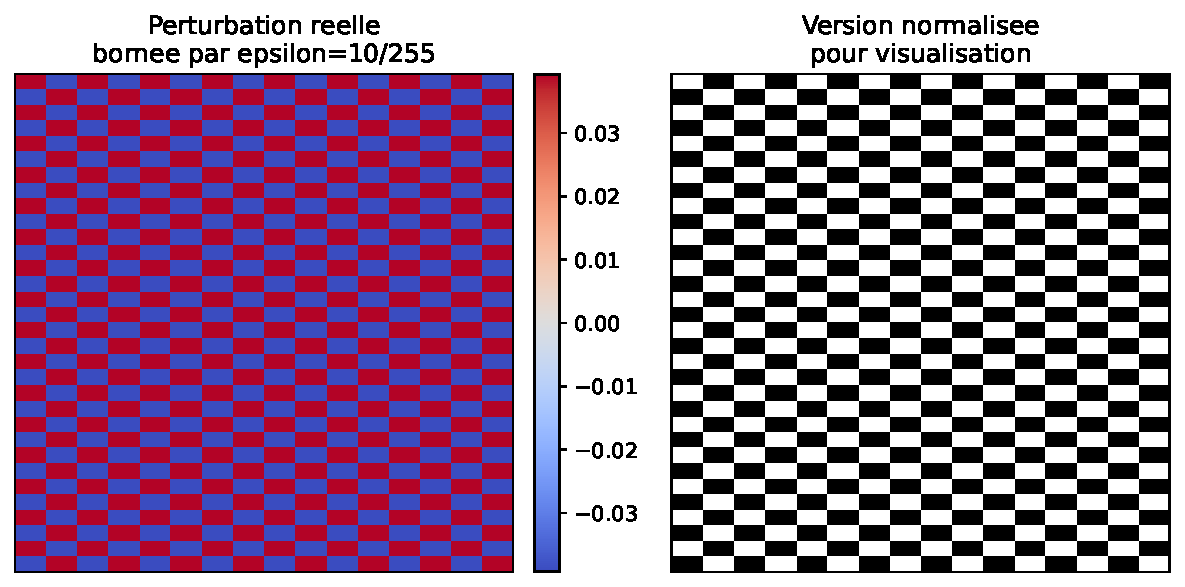
\includegraphics[width=0.55\textwidth]{figures/results/sfa_spatial_pattern_vgg_cifar10.pdf}
    \caption{Motif spatial associé à la perturbation SFA pour la fréquence $(16,24)$. La visualisation est
    normalisée afin de rendre la structure du motif visible.}
    \label{fig:sfa_spatial_pattern_vgg_cifar10}
\end{figure}

\section{Mesure de la sensibilité fréquentielle}
\label{sec:mesure_sensibilite_frequentielle}

Une fois les perturbations de Fourier définies, il faut mesurer leur effet sur le modèle.

\subsection{Définition du fool ratio}
\label{subsec:def_fool_ratio}

Soit $f$ le modèle étudié, et soit $\mathcal{D}=\{x_1,\dots,x_M\}$ un ensemble d'images. Pour une
fréquence $(u,v)$ donnée, on note $\tilde{x}_k^{(u,v)}$ l'image obtenue en ajoutant à $x_k$ la perturbation
de Fourier associée à cette fréquence.

Le \textit{fool ratio} mesure la proportion d'images pour lesquelles la prédiction du modèle change
après perturbation :
\[
    \operatorname{FR}(u,v)
    =
    \frac{1}{M}
    \sum_{k=1}^{M}
    \mathbf{1}
    \left[
        f(x_k) \neq f\!\left(\tilde{x}_k^{(u,v)}\right)
    \right].
\]

Cette mesure ne compare pas directement la prédiction au label réel. Elle compare uniquement la
prédiction du modèle avant et après perturbation. Ainsi, une image est comptée comme réussie pour
l'attaque lorsque la perturbation modifie la décision du modèle.

Le \textit{fool ratio} indique donc dans quelle mesure une direction fréquentielle est capable de modifier
les prédictions, indépendamment de la classe réelle des images.

% \subsection{Stabilité entre heatmaps}

% Pour comparer les heatmaps obtenues avec différentes seeds d'entraînement, nous utilisons deux
% mesures de corrélation. Chaque heatmap est d'abord aplatie en un vecteur de taille $32\times32$,
% contenant les \textit{fool ratios} de toutes les fréquences.

% La corrélation de Pearson mesure si deux heatmaps ont une structure globale similaire en valeur. La
% corrélation de Spearman compare plutôt l'ordre relatif des fréquences, en remplaçant les valeurs par
% leurs rangs. Elle permet donc de vérifier si les fréquences les plus sensibles restent globalement les
% mêmes d'un entraînement à l'autre, même lorsque les valeurs exactes des \textit{fool ratios} changent
% légèrement.

\subsection{Génération des heatmaps}
\label{subsec:generation_heatmaps}

Une heatmap de sensibilité fréquentielle est une matrice $H \in \mathbb{R}^{32\times32}$ dont chaque
case correspond à une fréquence $(u,v)$. La valeur $H_{u,v}$ est le \textit{fool ratio} obtenu lorsque
la perturbation de Fourier associée à cette fréquence est ajoutée aux images de test.

Le calcul suit trois étapes : d'abord, nous calculons les prédictions du modèle sur les images propres ;
ensuite, pour chaque fréquence, nous appliquons la perturbation correspondante ; enfin, nous mesurons
la proportion de prédictions modifiées. Cette procédure est résumée dans
l'algorithme~\ref{algo:algorithme_heatmap}.

\begin{algorithm}[H]
\caption{Génération d'une heatmap de sensibilité fréquentielle}
\label{algo:algorithme_heatmap}
\begin{algorithmic}
\State \textbf{input} : modèle $f$, images de test $\mathcal{D}$, amplitude $\epsilon$
\State \textbf{output} : heatmap $H \in \mathbb{R}^{32 \times 32}$
\State
\State $y \leftarrow f(\mathcal{D})$ \Comment{prédictions sur les images propres}
\For{$u = 0$ \textbf{to} $31$}
    \For{$v = 0$ \textbf{to} $31$}
        \State $\delta_{u,v} \leftarrow$ construire la perturbation de Fourier de fréquence $(u,v)$
        \State $\tilde{\mathcal{D}}_{u,v} \leftarrow \operatorname{clip}_{[0,1]}(\mathcal{D} + \delta_{u,v})$
        \State $\tilde{y}_{u,v} \leftarrow f(\tilde{\mathcal{D}}_{u,v})$
        \State $H_{u,v} \leftarrow \operatorname{FoolRatio}(y,\tilde{y}_{u,v})$
    \EndFor
\EndFor
\end{algorithmic}
\end{algorithm}

\subsection{Choix de la fréquence la plus sensible}
\label{subsec:choix_frequence_sensible}

Une fois la heatmap calculée, nous sélectionnons la fréquence qui maximise le \textit{fool ratio} :
\[
    (u^\star,v^\star)
    =
    \arg\max_{(u,v)}
    \operatorname{FR}(u,v).
\]

Cette fréquence correspond à la perturbation de Fourier la plus efficace parmi toutes celles testées
dans le protocole.

Cette sélection est effectuée séparément pour CIFAR-10 et CIFAR-100. Les fréquences obtenues et
leur interprétation sont présentées dans la section~\ref{subsec:frequences_plus_sensibles}.

\section{Résultats expérimentaux}
\label{sec:resultats_experimentaux}

\subsection{Heatmaps de sensibilité fréquentielle}
\label{subsec:resultats_heatmaps}

La méthodologie décrite précédemment nous permet de construire les cartes de sensibilité fréquentielle
du modèle \texttt{VGGSmallBN}. La figure~\ref{fig:heatmap_comparison_vgg_cifar10_cifar100}
compare les résultats obtenus sur nos deux datasets pour une même amplitude de perturbation,
fixée à $\epsilon = 10/255$.

\begin{figure}[H]
    \centering
    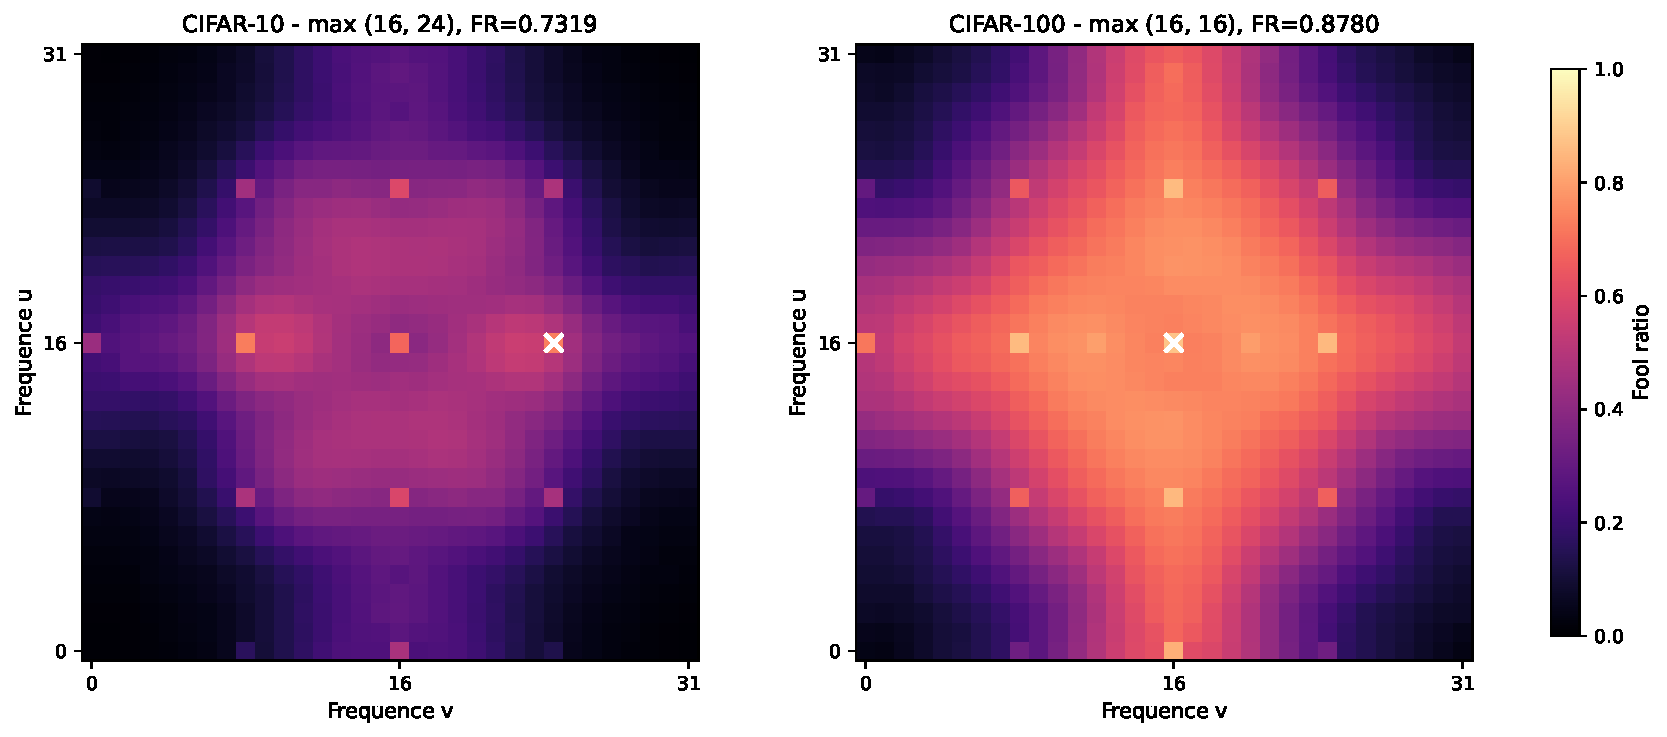
\includegraphics[width=0.7\textwidth]{figures/results/fourier_heatmap_comparison_vgg_cifar10_cifar100.pdf}
    \caption{Heatmaps de sensibilité fréquentielle pour \texttt{VGGSmallBN} sur CIFAR-10 et CIFAR-100.}
    \label{fig:heatmap_comparison_vgg_cifar10_cifar100}
\end{figure}
L'observation principale est que la sensibilité n'est pas uniforme dans le domaine de Fourier. Certaines
fréquences provoquent très peu de changements de prédiction, tandis que d'autres produisent un
\textit{fool ratio} beaucoup plus élevé.

Les deux heatmaps présentent une organisation structurée, avec des zones de forte sensibilité autour
de certaines lignes et intersections fréquentielles, notamment près des coordonnées liées à $16$. Cette
structure suggère que la vulnérabilité du modèle n'est pas un effet aléatoire, mais dépend de certaines
directions fréquentielles privilégiées.

Une comparaison descriptive avec le spectre moyen des images propres est donnée en
annexe~\ref{annexe:spectres_moyens_cifar}. Cette analyse vise a donne une autre manière d'interpréter
les résultats sous le prisme des statistiques fréquentielles des données brutes.

Pour compléter la lecture des heatmaps, la figure~\ref{fig:fool_ratio_histogram_comparison_vgg_cifar10_cifar100}
représente la distribution des \textit{fool ratios} sur les $32 \times 32 = 1024$ fréquences testées.

Sur CIFAR-10, la plupart des fréquences ont un effet faible ou modéré, et seules quelques directions
atteignent des \textit{fool ratios} élevés. La sensibilité du modèle est donc réelle, mais relativement
localisée dans le domaine fréquentiel.

\begin{figure}[H]
    \centering
    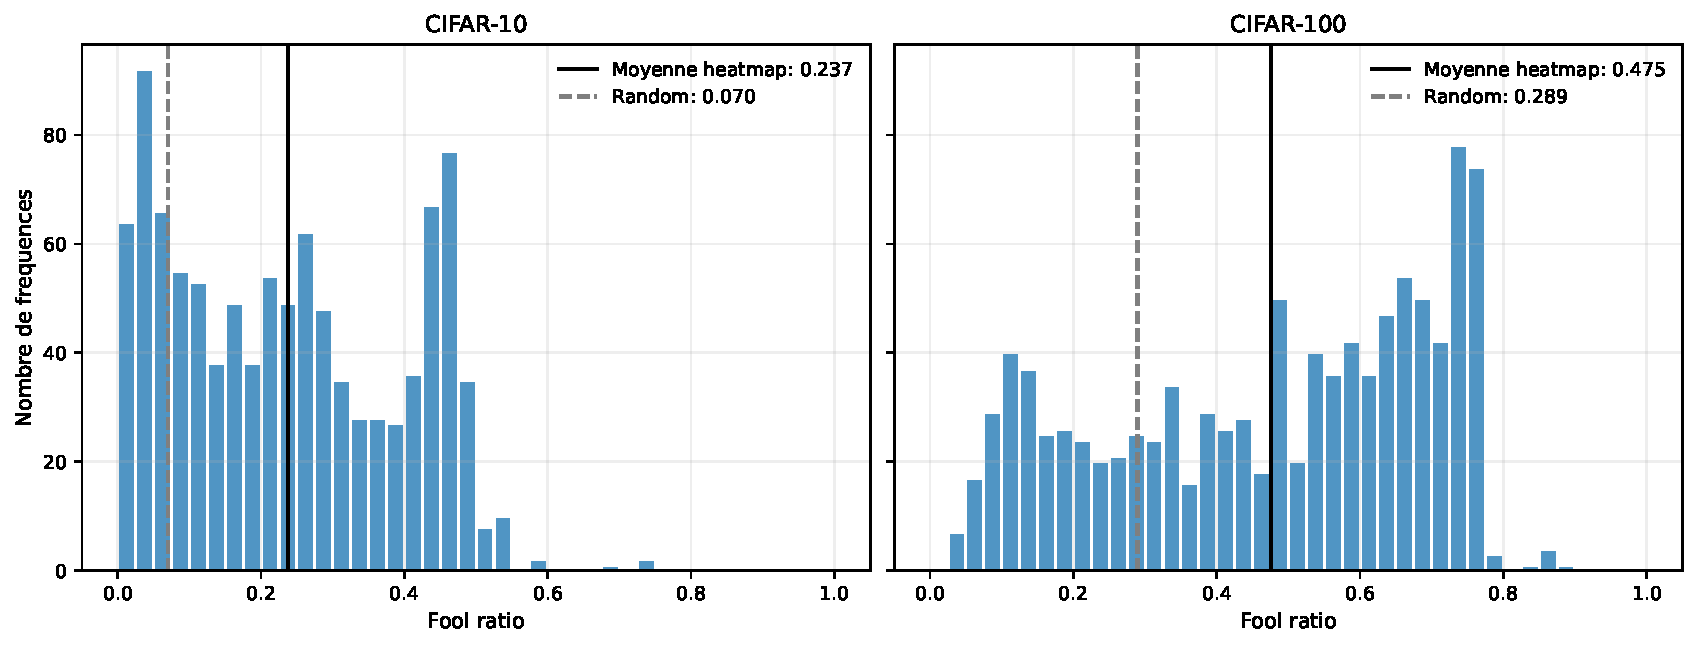
\includegraphics[width=0.9\textwidth]{figures/results/fourier_fool_ratio_histogram_comparison_vgg_cifar10_cifar100.pdf}
    \caption{Distribution des \textit{fool ratios} obtenus sur l'ensemble des fréquences de Fourier testées.}
    \label{fig:fool_ratio_histogram_comparison_vgg_cifar10_cifar100}
\end{figure}

Sur CIFAR-100, la distribution est déplacée vers la droite : la moyenne passe de $0.2375$ à $0.4755$.
Le modèle est donc globalement plus fragile, ce qui est cohérent avec la difficulté plus élevée de la
tâche discutée en annexe~\ref{annexe:marges-logits}. Cependant, cette fragilité reste structurée : toutes les fréquences ne produisent pas le même
effet, et certaines directions demeurent nettement plus perturbatrices que d'autres.

L'histogramme complète donc la lecture visuelle des heatmaps. Il montre que la sensibilité n'est pas
seulement non uniforme spatialement : elle est aussi très dispersée quantitativement. Une petite partie
des fréquences concentre l'essentiel de l'effet perturbateur.

\subsection{Fréquences les plus sensibles}
\label{subsec:frequences_plus_sensibles}

L'analyse des heatmaps permet d'identifier les fréquences les plus perturbatrices pour chaque
dataset. Le tableau~\ref{tab:frequences_plus_sensibles} présente les trois fréquences obtenant les
plus grands \textit{fool ratios}.

\begin{table}[H]
    \centering
    \begin{tabular}{c|cc|cc}
        & \multicolumn{2}{c|}{CIFAR-10} & \multicolumn{2}{c}{CIFAR-100} \\
        Rang & Fréquence $(u,v)$ & \textit{Fool ratio} & Fréquence $(u,v)$ & \textit{Fool ratio} \\
        \hline
        1 & $(16,24)$ & $0.7319$ & $(16,16)$ & $0.8780$ \\
        2 & $(16,8)$  & $0.7295$ & $(16,8)$  & $0.8585$ \\
        3 & $(16,16)$ & $0.6765$ & $(24,16)$ & $0.8565$ \\
    \end{tabular}
    \caption{Fréquences les plus sensibles pour \texttt{VGGSmallBN} sur CIFAR-10 et CIFAR-100.}
    \label{tab:frequences_plus_sensibles}
\end{table}

Les fréquences dominantes se concentrent autour d'une même famille de directions. Sur CIFAR-10, les deux premières fréquences,
$(16,24)$ et $(16,8)$, sont conjuguées modulo $32$ et obtiennent logiquement des \textit{fool ratios} presque
identiques. 

Sur CIFAR-100, la fréquence la plus sensible devient $(16,16)$, qui est sa propre conjuguée modulo
$32$.

\subsection{Stabilité des zones sensibles entre plusieurs entraînements}
\label{subsec:stabilite_multi_seeds}

Les heatmaps précédentes montrent que certaines fréquences sont beaucoup plus sensibles que
d'autres. Cependant, une question importante reste à vérifier : cette structure est-elle propre à un
entraînement particulier du modèle, ou reste-t-elle observable lorsque l'on change la seed
d'initialisation ?

\begin{figure}[H]
    \centering
    \vspace{-10pt} 

    \begin{minipage}{0.35\textwidth}
        \centering
        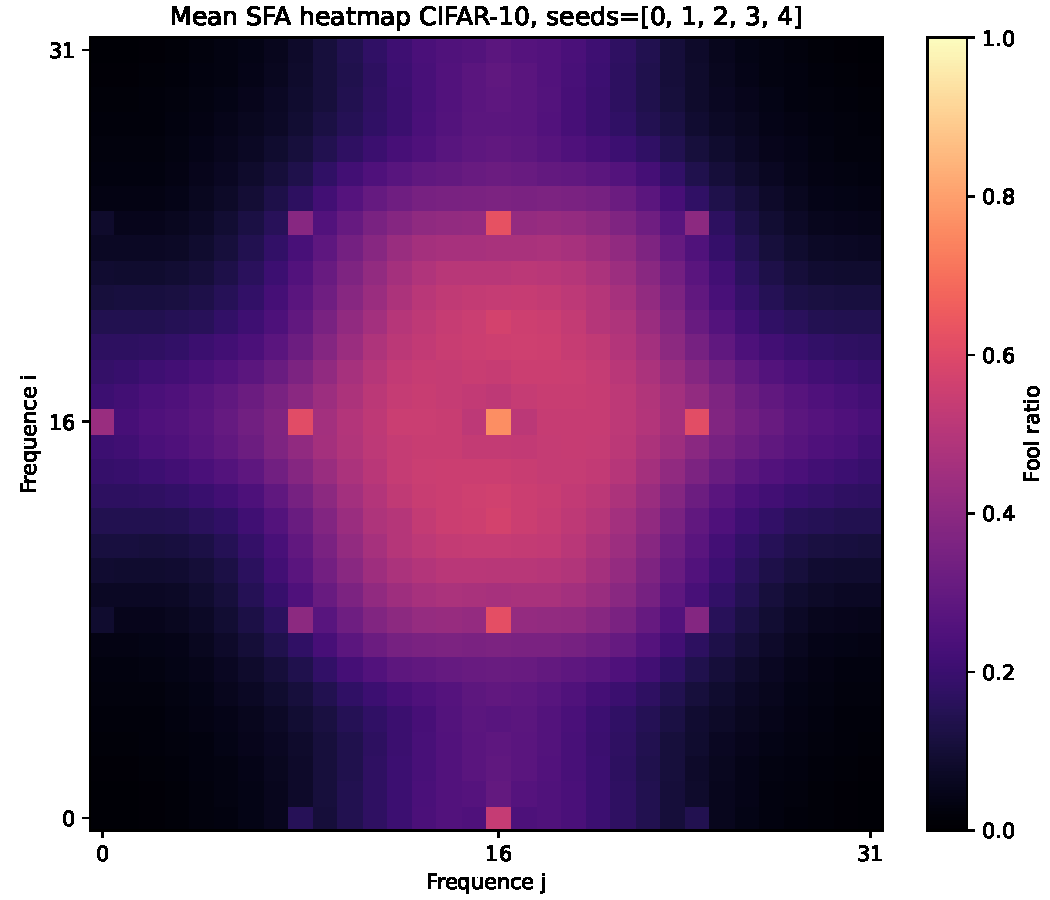
\includegraphics[width=\textwidth]{figures/results/stability_cifar10_heatmap_mean.pdf}
        \vspace{-5pt} 
        {\small (a) CIFAR-10 -- \textit{fool ratio} moyen}
    \end{minipage}
    \hspace{0.05\textwidth} 
    \begin{minipage}{0.35\textwidth}
        \centering
        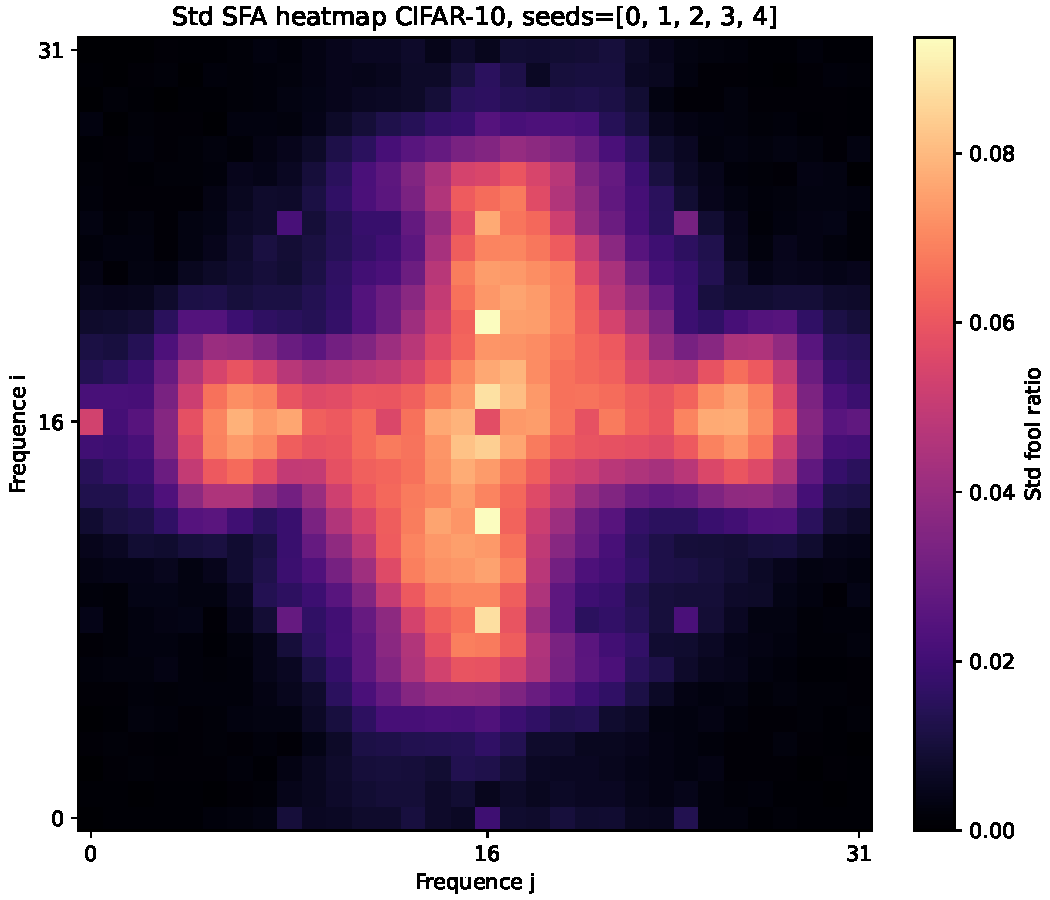
\includegraphics[width=\textwidth]{figures/results/stability_cifar10_heatmap_std.pdf}
        \vspace{-5pt}
        {\small (b) CIFAR-10 -- écart-type}
    \end{minipage}

    \vspace{2pt} 

    \begin{minipage}{0.35\textwidth}
        \centering
        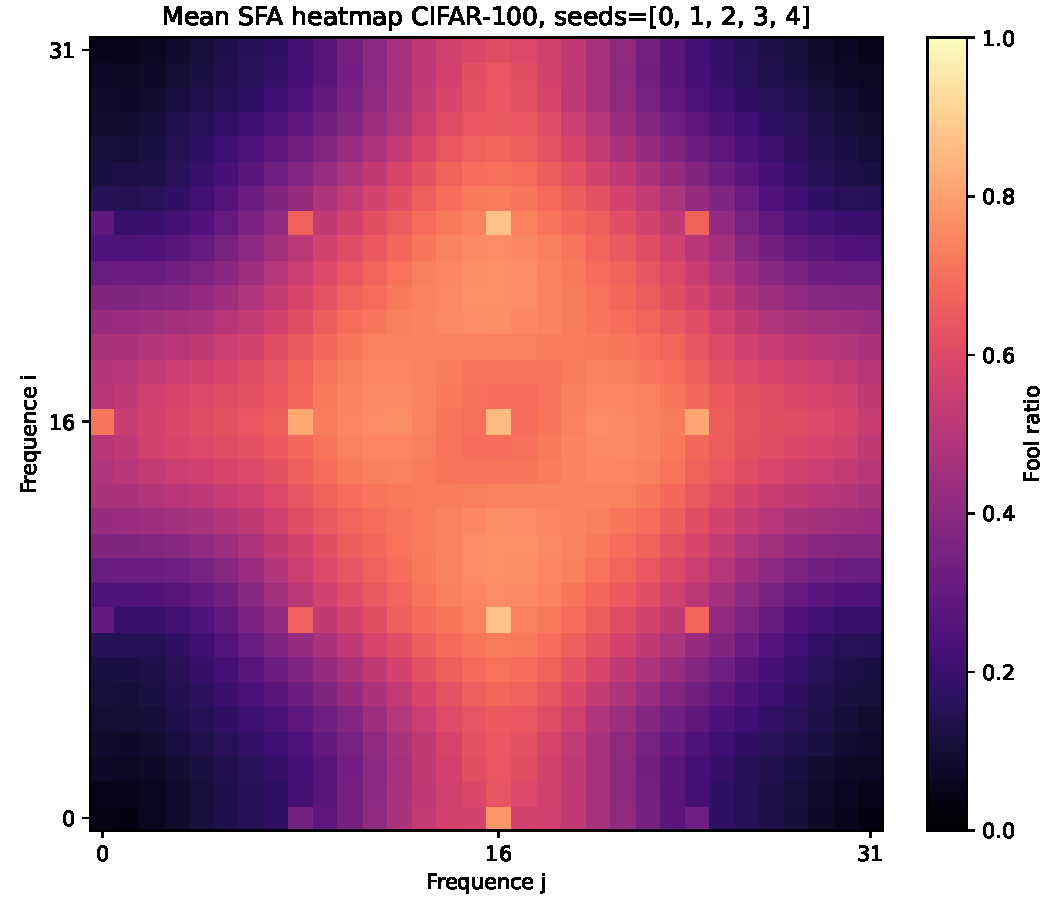
\includegraphics[width=\textwidth]{figures/results/stability_cifar100_heatmap_mean.pdf}
        \vspace{-5pt}
        {\small (c) CIFAR-100 -- \textit{fool ratio} moyen}
    \end{minipage}
    \hspace{0.05\textwidth}
    \begin{minipage}{0.35\textwidth}
        \centering
        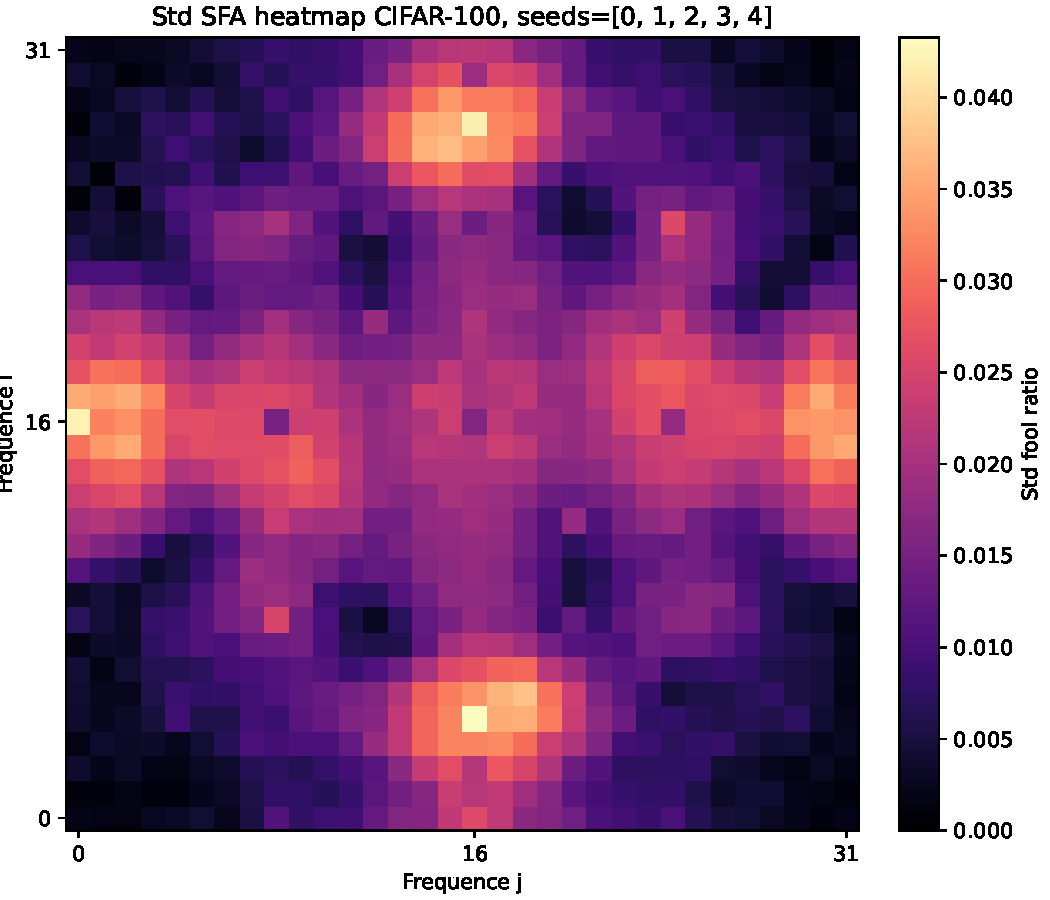
\includegraphics[width=\textwidth]{figures/results/stability_cifar100_heatmap_std.pdf}
        \vspace{-5pt}
        {\small (d) CIFAR-100 -- écart-type}
    \end{minipage}

    \caption{Stabilité de la sensibilité fréquentielle de \texttt{VGGSmallBN} sur CIFAR-10 et CIFAR-100.}
    \label{fig:stability_cifar10_cifar100_mean_std}
\end{figure}

Pour répondre à cette question, nous avons répété l'expérience sur CIFAR-10 et CIFAR-100 avec cinq
entraînements indépendants de \texttt{VGGSmallBN}. Le protocole d'entraînement est conservé identique
pour chaque run. Seule la seed est modifiée.

La figure~\ref{fig:stability_cifar10_cifar100_mean_std} présente,
pour chaque dataset, la heatmap moyenne obtenue sur les cinq seeds ainsi que l'écart-type associé
à chaque fréquence.

Les résultats montrent que la structure globale des heatmaps reste très stable entre les entraînements.
Sur CIFAR-10, les zones de forte sensibilité restent localisées autour des mêmes régions fréquentielles,
en particulier autour des fréquences médianes liées aux axes centraux. Sur CIFAR-100, cette structure
est encore plus marquée : une large zone de forte sensibilité apparaît autour des fréquences centrales.

% Cette stabilité est confirmée quantitativement par les corrélations entre heatmaps. Sur CIFAR-10, la
% corrélation de Pearson moyenne entre heatmaps est d'environ $0.976$, et la corrélation de Spearman
% moyenne d'environ $0.985$. Sur CIFAR-100, ces valeurs montent respectivement à environ $0.994$
% et $0.992$. Les heatmaps sont donc très proches d'un entraînement à l'autre, aussi bien en valeur
% qu'en classement relatif des fréquences.

Le tableau~\ref{tab:stability_multiseed_metrics} résume les principales métriques moyennées sur les cinq
seeds. L'accuracy propre reste proche de celle du modèle principal, tandis que l'accuracy après attaque
diminue fortement. Cela montre que le \textit{fool ratio} élevé correspond bien à une dégradation réelle
des performances du modèle, et pas seulement à des changements de prédiction sans conséquence sur
la classification correcte.

\begin{table}[H]
    \centering
    \begin{tabular}{l|c|c}
        \hline
        Métrique & CIFAR-10 & CIFAR-100 \\
        \hline
        Accuracy propre moyenne & $93.08\,\%$ & $72.50\,\%$ \\
        Meilleur \textit{fool ratio} moyen & $76.35\,\%$ & $87.64\,\%$ \\
        Accuracy après attaque moyenne & $23.39\,\%$ & $11.83\,\%$ \\
        Taux de succès sur images initialement correctes & $76.38\,\%$ & $85.18\,\%$ \\
        % Corrélation de Pearson moyenne entre heatmaps & $0.976$ & $0.994$ \\
        % Corrélation de Spearman moyenne entre heatmaps & $0.985$ & $0.992$ \\
        \hline
    \end{tabular}
    \caption{Résumé de l'expérience de stabilité multi-seeds sur CIFAR-10 et CIFAR-100.}
    \label{tab:stability_multiseed_metrics}
\end{table}

\subsection{Amplification interne des fréquences sensibles}
\label{subsec:amplification_interne_sfa}

Les heatmaps précédentes montrent que certaines fréquences de Fourier produisent des \textit{fool ratios}
nettement plus élevés que d'autres. Pour mieux comprendre ce phénomène, nous avons analysé la manière
dont ces perturbations se propagent à l'intérieur du réseau.

Pour une perturbation \(\delta\), nous notons \(G_l(\delta)\) l'amplification normalisée mesurée à la
couche \(l\). Cette quantité compare la norme moyenne de la variation d'activation provoquée par la
perturbation à la norme de la perturbation d'entrée. Elle permet donc de comparer l'effet relatif de
différentes fréquences dans les blocs internes du réseau et au niveau des logits.

Afin de rendre cette analyse plus robuste, nous l'avons répétée sur les cinq checkpoints utilisés dans
l'expérience de stabilité multi-seeds. Les fréquences sont regroupées à partir de la heatmap moyenne :
les \(50\) fréquences les plus sensibles, \(50\) fréquences de sensibilité intermédiaire, et les \(50\)
fréquences les moins sensibles. La fréquence principale correspond à la meilleure fréquence moyenne
sur les cinq seeds.

\begin{figure}[H]
    \centering
    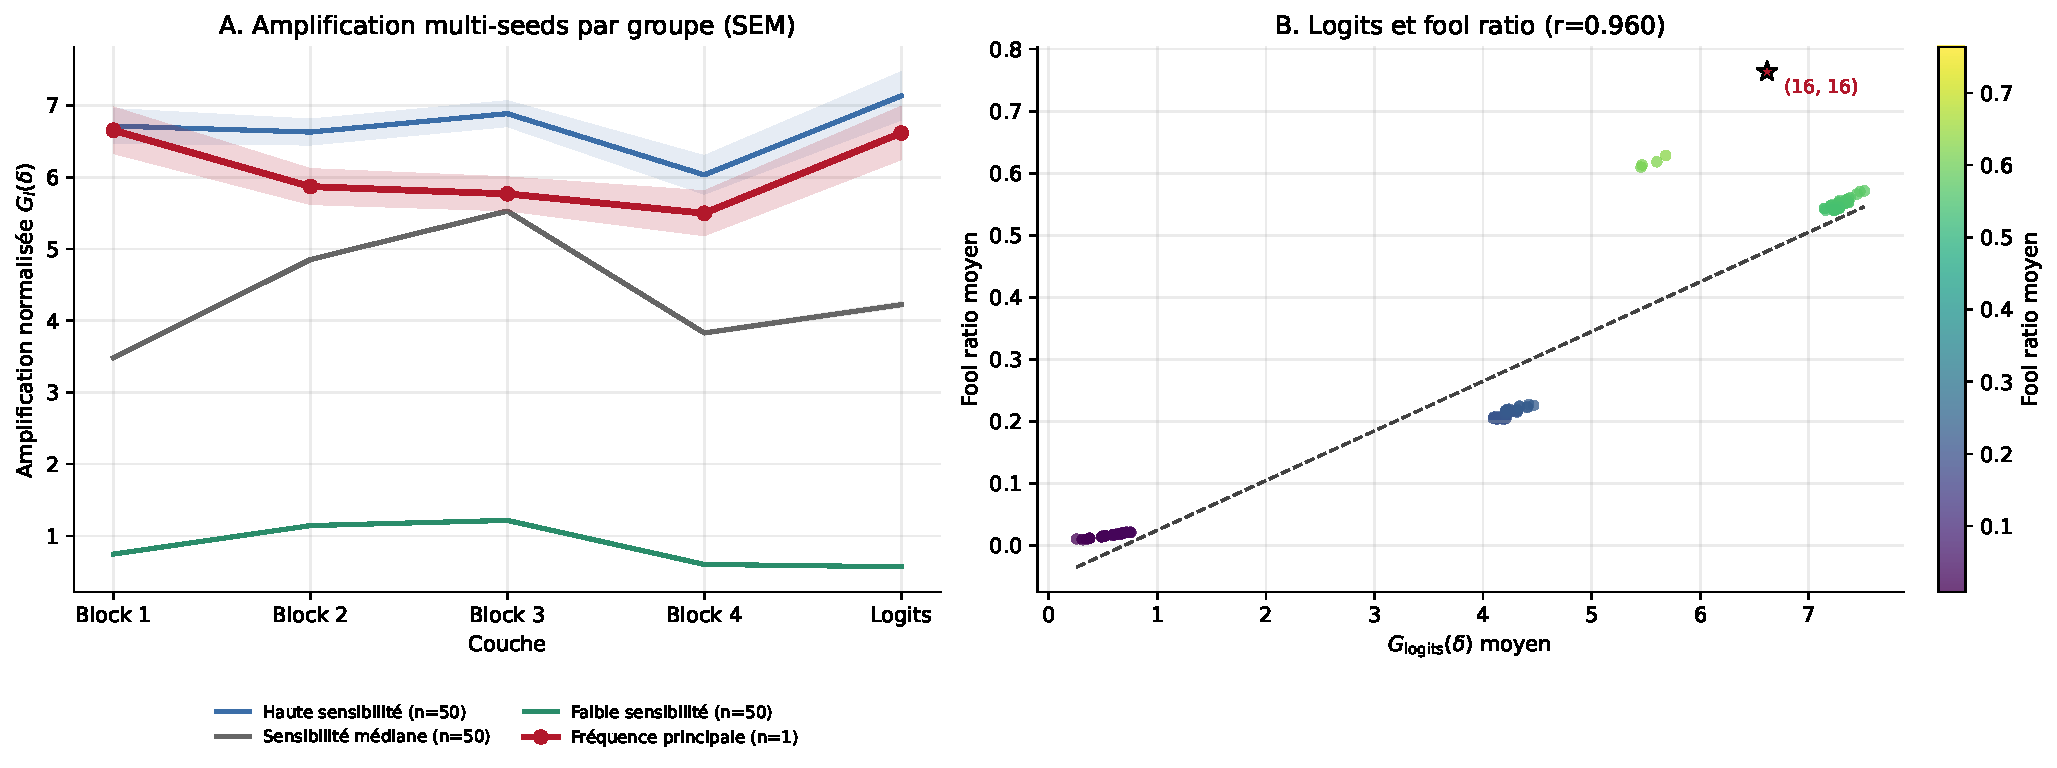
\includegraphics[width=\textwidth]{figures/results/layerwise_frequency_sensitivity_analysis_vgg_cifar10_multiseed.pdf}
    \caption{Analyse multi-seeds de l'amplification interne des perturbations de Fourier dans
    \texttt{VGGSmallBN} sur CIFAR-10. À gauche, les fréquences sont regroupées selon leur
    \textit{fool ratio} moyen. Les bandes indiquent l'erreur standard sur les cinq seeds. À droite,
    l'amplification moyenne au niveau des logits est comparée au \textit{fool ratio} moyen.}
    \label{fig:layerwise_frequency_sensitivity_multiseed}
\end{figure}

La figure~\ref{fig:layerwise_frequency_sensitivity_multiseed} montre que logiquement les fréquences les plus
sensibles sont aussi celles qui produisent les amplifications internes les plus élevées. 

Le panneau de droite montre une corrélation élevée entre l'amplification moyenne au niveau des logits
et le \textit{fool ratio} moyen. Cela suggère que la sensibilité finale du modèle n'est pas seulement liée
au couple $(u, v)$ choisi, mais aussi à la manière dont cette perturbation est propagée et
amplifiée par le réseau.

Cette observation fait le lien avec le cadre théorique et avec l'interprétation locale introduite au
chapitre précédent : même si le réseau réel n'est pas globalement linéaire, certaines directions
fréquentielles semblent être davantage amplifiées par son comportement local, ce qui peut expliquer
leur effet plus important sur les prédictions.

Une visualisation plus détaillée des heatmaps internes par couche est donnée en annexe~\ref{annexe:heatmaps_internes_couches}.

\subsection{Comparaison avec un bruit aléatoire}
\label{subsec:comparaison_bruit_aleatoire}

Pour vérifier que les fortes valeurs obtenues par la SFA ne proviennent pas uniquement de l'amplitude
de la perturbation, nous comparons la meilleure direction de Fourier avec une baseline de bruit
aléatoire. Dans cette baseline, chaque pixel est perturbé indépendamment par un bruit uniforme
borné dans le même intervalle d'amplitude. La contrainte est donc la même que pour la SFA :
\[
    \|\delta\|_{\infty} \leq \epsilon,
    \qquad
    \epsilon = 10/255.
\]
La différence vient de la structure de la perturbation : la SFA utilise un motif fréquentiel cohérent,
tandis que la baseline aléatoire ne privilégie aucune direction particulière.

\textbf{A FAIRE : }
Il faudrais s'assurer que  $\|\delta_{SFA}\|_{2} = \|\delta_{random}\|_{2}$

La figure~\ref{fig:sfa_vs_random_comparison_vgg_cifar10_cifar100} compare, pour chaque dataset,
le \textit{fool ratio} de la meilleure fréquence SFA avec le \textit{fool ratio} moyen obtenu par bruit
aléatoire.

\begin{figure}[H]
    \centering
    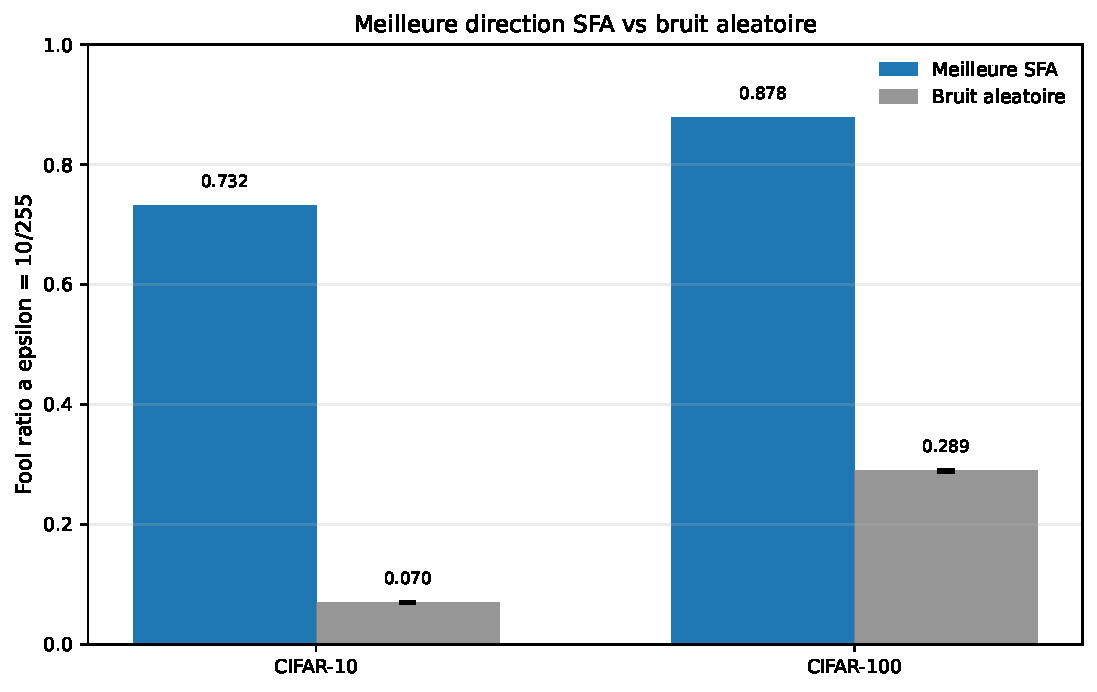
\includegraphics[width=0.85\textwidth]{figures/results/sfa_vs_random_comparison_vgg_cifar10_cifar100.pdf}
    \caption{Comparaison entre la meilleure direction SFA et un bruit aléatoire uniforme de même amplitude
    $\epsilon = 10/255$. Pour le bruit aléatoire, la barre d'erreur représente l'écart-type sur 100 essais.}
    \label{fig:sfa_vs_random_comparison_vgg_cifar10_cifar100}
\end{figure}

Sur CIFAR-10, la différence est très nette : la meilleure direction de Fourier atteint un
\textit{fool ratio} de $0.7319$, alors que le bruit aléatoire moyen atteint seulement $0.0704$.
La perturbation de Fourier est donc environ dix fois plus efficace qu'un bruit aléatoire de même
amplitude. Ce résultat indique que la vulnérabilité observée ne peut pas être expliquée par la seule
taille de la perturbation.

Sur CIFAR-100, le bruit aléatoire est déjà plus perturbateur, avec un \textit{fool ratio} moyen de
$0.2892$. Confirment que le modèle entraîné sur CIFAR-100 est globalement plus fragile. Cependant,
la meilleure direction SFA atteint $0.8780$, soit environ trois fois le niveau du bruit aléatoire moyen.

\subsection{Effet de l'amplitude de la perturbation}
\label{subsec:effet_amplitude_epsilon}

Jusqu'ici, les résultats principaux ont été obtenus avec $\epsilon = 10/255$. Cette valeur permet de
comparer nos résultats au protocole original, mais elle peut produire des motifs visibles sur des images
de très faible résolution. Or une attaque adversariale a pour but de rester
peu perceptible pour l'humain. Nous testons donc si les fréquences les plus sensibles conservent un effet pour des
valeurs plus faibles de $\epsilon$.

Pour cela, nous fixons la fréquence la plus sensible de chaque dataset, puis nous faisons varier
$\epsilon$ dans l'ensemble suivant :
\[
    \epsilon \in
    \left\{
        \frac{1}{255},
        \frac{2}{255},
        \frac{3}{255},
        \frac{5}{255},
        \frac{10}{255}
    \right\}.
\]

\begin{figure}[H]
    \centering
    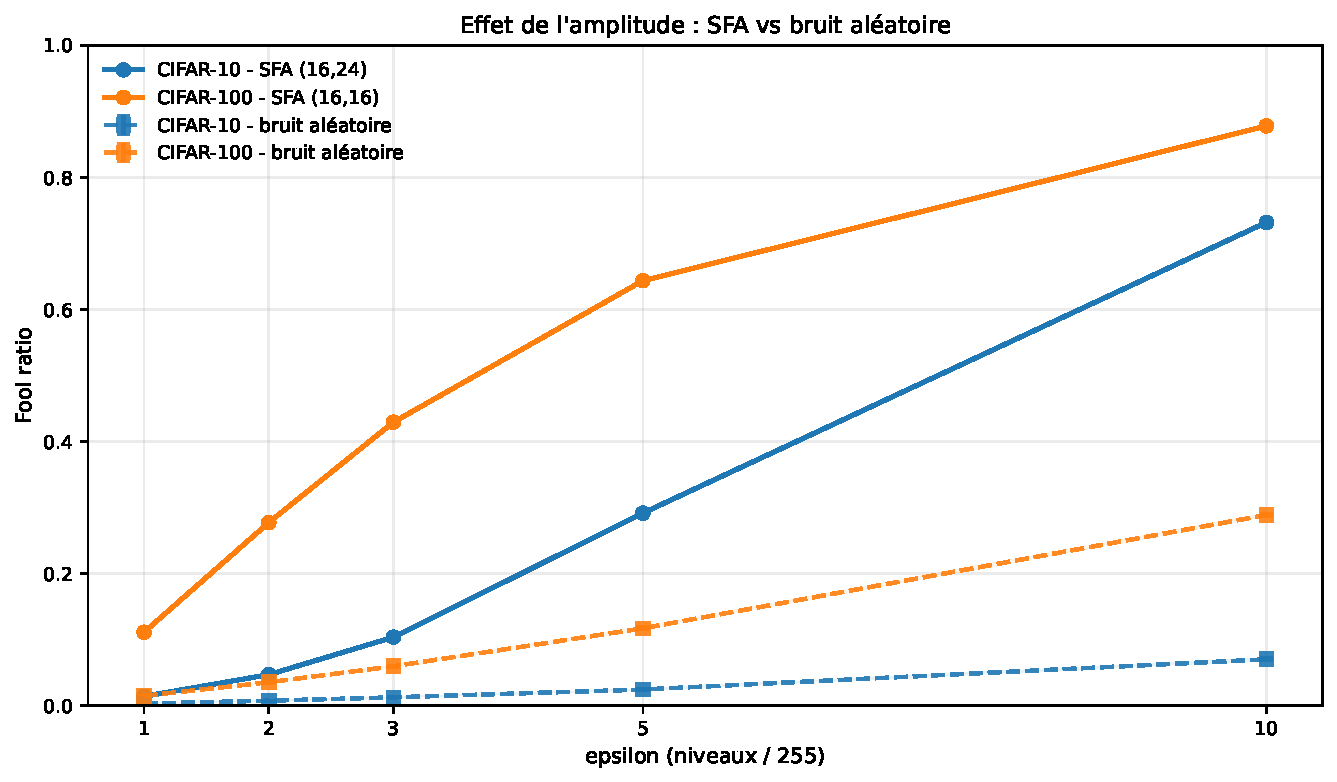
\includegraphics[width=0.55\textwidth]{figures/results/sfa_epsilon_sweep_with_random_comparison_vgg_cifar10_cifar100.pdf}
    \caption{Évolution du \textit{fool ratio} en fonction de l'amplitude $\epsilon$ pour la meilleure fréquence
    SFA de chaque dataset.}
    \label{fig:sfa_epsilon_sweep_comparison_vgg_cifar10_cifar100}
\end{figure}

La figure~\ref{fig:sfa_epsilon_sweep_comparison_vgg_cifar10_cifar100} montre une augmentation
régulière du \textit{fool ratio} lorsque $\epsilon$ augmente. Ce comportement est attendu : plus la
perturbation est grande, plus elle modifie l'image d'entrée, et plus elle a de chances de déplacer la
prédiction du modèle. Mais elle confirme aussi que dans ce contexte, l'amplitude de la perturbation 
est un facteur important de l'efficacité de l'attaque, nous obligeant rendre la perturbation plus moins
discrète pour obtenir un effet plus significatif.

\begin{figure}[H]
    \centering
    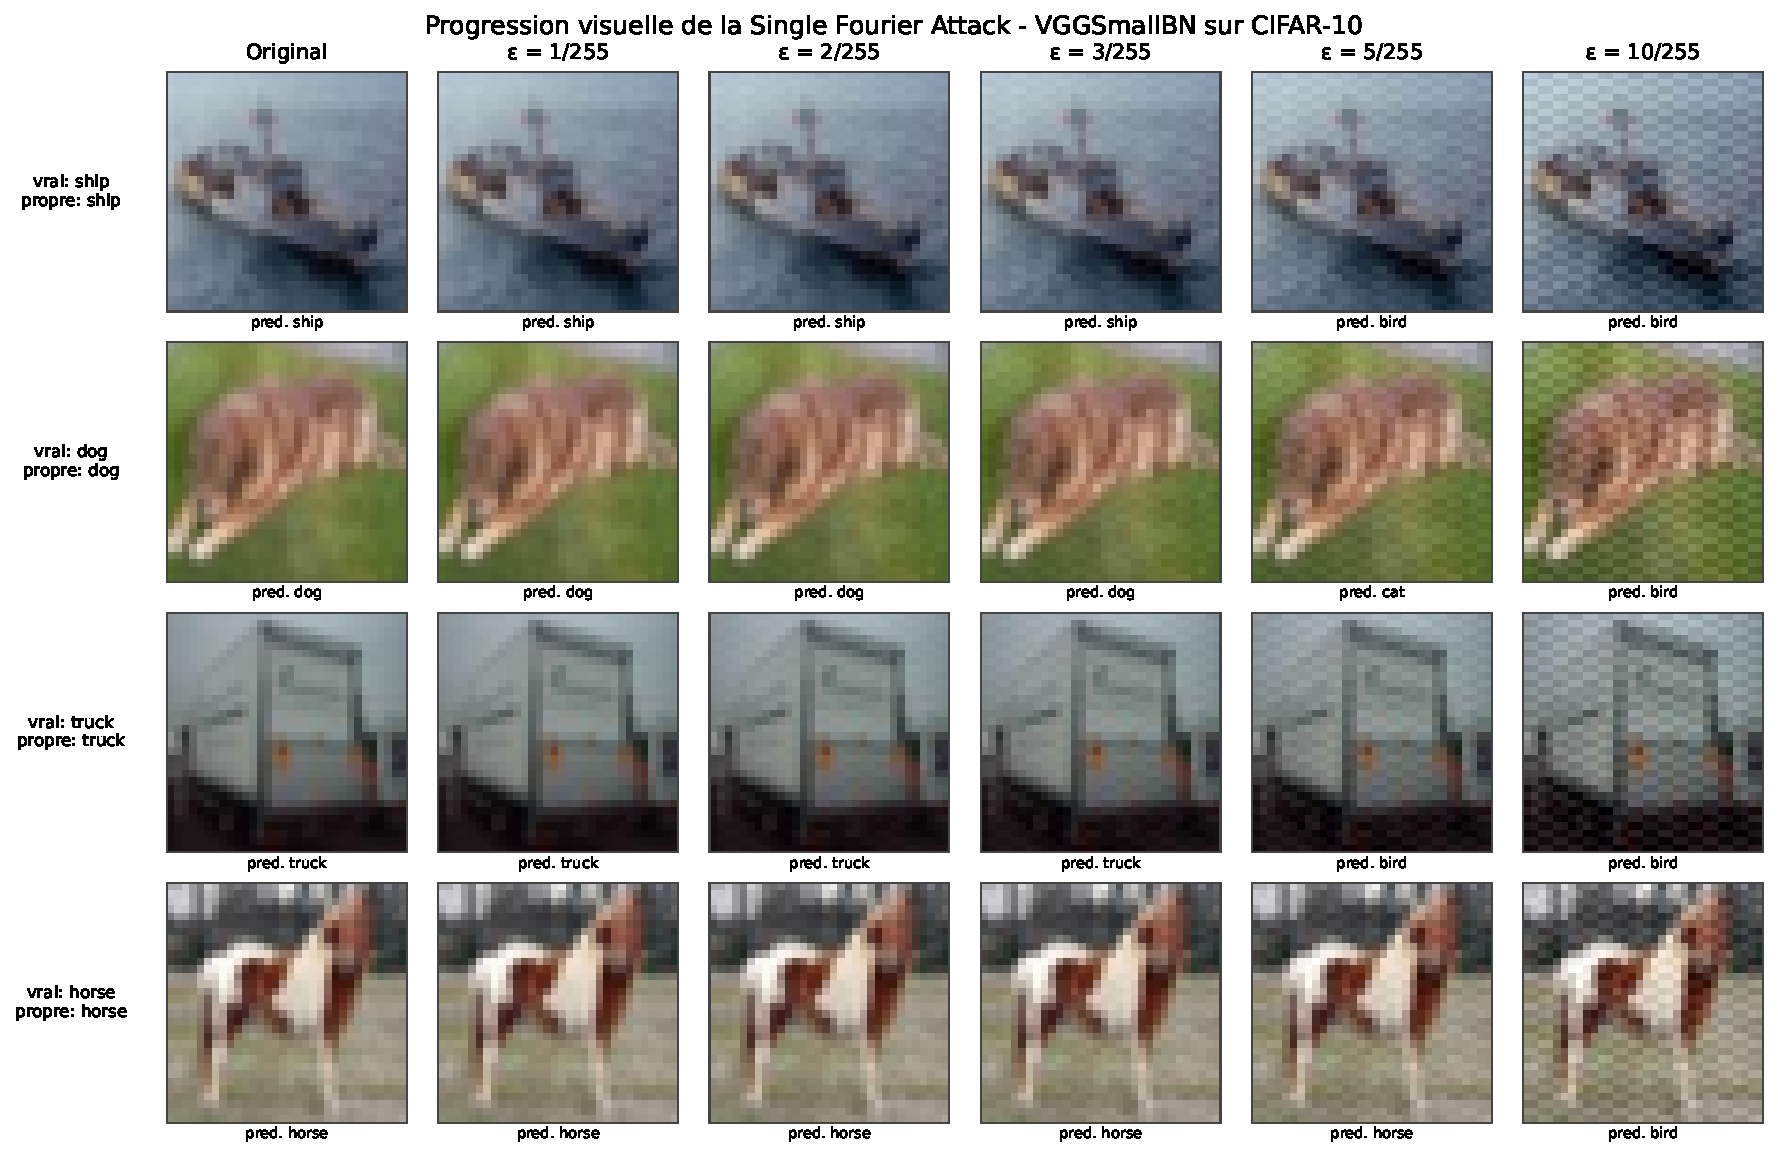
\includegraphics[width=1\textwidth]{figures/results/sfa_visual_progression_vgg_cifar10.pdf}
    \caption{Progression visuelle d'une attaque \textit{Single Fourier Attack} sur des images de CIFAR-10.}
    \label{fig:sfa_visual_progression_vgg_cifar10}
\end{figure}

Comme l'illustre la figure~\ref{fig:sfa_visual_progression_vgg_cifar10}, l'augmentation de l'amplitude rend le motif de 
Fourier de plus en plus intrusif. On remarque notamment qu'à partir d'une valeur de $\epsilon = 3/255$, la perturbation 
structurée en forme de grille commence à être distinctement visible à l'oeil nu. 

Il convient néanmoins de nuancer ces observations. Les expériences sont réalisées sur des images de
très basse résolution ($32\times32$ pixels) et avec une architecture volontairement restreinte
(\texttt{VGGSmallBN}). Les conclusions ne doivent donc pas être généralisées directement à des images
de haute résolution ou à des architectures beaucoup plus profondes. Elles montrent cependant que,
dans notre cadre expérimental, l'effet des perturbations de Fourier dépend fortement de l'amplitude.

\subsection{Lien avec le cadre théorique}
\label{subsec:discussion_lien_cadre_theorique}

Les résultats expérimentaux obtenus dans ce chapitre permettent de revenir au cadre théorique
développé au chapitre précédent. Dans le modèle linéaire idéalisé, les fonctions de Fourier apparaissent
comme des directions privilégiées des opérateurs de convolution. Dans un CNN réel, cette propriété
ne s'applique plus directement au réseau complet, mais elle peut rester pertinente localement à travers
le jacobien du modèle.

Les heatmaps obtenues expérimentalement vont dans ce sens. Si toutes les directions fréquentielles
étaient équivalentes pour le modèle, les cartes de sensibilité seraient beaucoup plus uniformes. Or ce
n'est pas ce que l'on observe : certaines fréquences produisent des \textit{fool ratios} nettement plus
élevés que d'autres, alors que toutes les perturbations respectent la même contrainte $\ell_\infty$.

La stabilité multi-seeds renforce cette interprétation. Les zones sensibles ne semblent pas dépendre
uniquement d'une initialisation particulière du réseau : elles restent visibles lorsque l'entraînement est
répété avec différentes seeds. La comparaison avec le bruit aléatoire montre également que l'effet ne
provient pas seulement de l'amplitude de la perturbation, mais de sa structure fréquentielle.

Ces résultats montrent que l'intuition issue du cadre théorique reste
observable expérimentalement pour \texttt{VGGSmallBN} : certaines directions de Fourier sont plus perturbatrices que d'autres,
ce qui est compatible avec une amplification locale de ces directions dans le réseau.

\paragraph{Influence du mélange entre canaux.}

Precedement nous avions considéré qu'une direction sensible peut aussi faire intervenir un mélange entre
les canaux couleur, sous la forme $a \otimes \varphi_{u,v}$. Le protocole principal utilise une version simplifiée de
cette idée : le même motif de Fourier est appliqué aux trois canaux, ce qui correspond à une direction
couleur de type $(1,1,1)$.

Une analyse complémentaire de cette simplification est proposée en annexe~\ref{annexe:color_sfa}.
Elle vise à montrer que le choix du mélange entre canaux est negligeable en comparaison du choix de maximiser l'amplification de l'attaque.

\section{Synthèse du chapitre}
\label{sec:synthese_chapitre4}

Les expériences réalisées confirment que la sensibilité de \texttt{VGGSmallBN} aux perturbations de
Fourier est fortement non uniforme. Sur CIFAR-10 comme sur CIFAR-100, certaines fréquences
provoquent beaucoup plus de changements de prédiction que d'autres, alors que toutes les perturbations
respectent la même contrainte $\ell_\infty$.

Cette structure reste stable entre plusieurs entraînements indépendants et dépasse nettement l'effet
obtenu avec un bruit aléatoire de même amplitude. Le balayage de $\epsilon$ montre toutefois que
l'efficacité de l'attaque dépend fortement de l'amplitude, en particulier sur des images de basse
résolution comme celles de CIFAR.

Enfin, l'analyse interne suggère que les fréquences les plus sensibles sont aussi celles qui sont le plus
amplifiées dans les représentations du réseau. Ces observations ne prouvent pas que le modèle réel se
comporte comme un opérateur linéaire global, mais elles montrent que la structure fréquentielle mise
en évidence dans le cadre théorique reste partiellement visible dans le comportement local du modèle.

\chapter{Conclusion}

Ce travail visait à explorer le lien intrinsèque entre la structure convolutionnelle des réseaux 
de neurones (CNN) et l'émergence de directions de vulnérabilité privilégiées dans le domaine de 
Fourier. Plus précisément, notre démarche a consisté à déterminer dans quelle mesure les propriétés 
mathématiques inhérentes aux couches de convolution — au-delà des biais liés aux données ou au 
processus d'entraînement — permettent d'expliquer l'existence de perturbations adversariales universelles.

Pour ce faire, après avoir posé le cadre général des CNN et des attaques adversariales, nous 
avons reconstruit et analysé le raisonnement théorique proposé par Tsuzuku et 
Sato~\cite{tsuzuku2019structural}, en nous appuyant initialement sur un modèle linéaire simplifié.

Afin de transposer ces résultats théoriques à l'architecture réelle des CNN, où la 
présence d'activations ReLU et d'opérations de \textit{max-pooling} empêche toute 
diagonalisation globale, nous avons introduit le concept de linéarisation locale via 
l'analyse du jacobien du modèle. Cette extension théorique s'est avérée cruciale pour 
justifier l'application de résultats fondés sur la linéarité à des architectures 
fondamentalement non linéaires.

L'ensemble de ces observations permet ainsi d'élucider le mécanisme par lequel une 
perturbation fondée sur une unique fréquence de Fourier peut impacter si sévèrement 
un réseau convolutionnel. L'amplification successive de cette perturbation au travers 
des différentes couches offre une explication structurelle probante à l'existence des 
perturbations universelles.

Notre démarche expérimentale vient conforter cette intuition. Les \textit{heatmaps} 
générées sur l'architecture \texttt{VGGSmallBN}, pour les jeux de données CIFAR-10 et 
CIFAR-100, mettent en évidence une sensibilité fréquentielle fortement hétérogène. 
Certaines fréquences engendrent en effet des \textit{fool ratios} significativement 
supérieurs, démontrant que des perturbations d'amplitude égale n'ont pas un impact 
équivalent : leur direction dans l'espace des entrées est un facteur déterminant. 
La comparaison de ces résultats avec l'injection d'un bruit aléatoire de même amplitude 
corrobore pleinement cette asymétrie.

Par ailleurs, les résultats soulignent l'influence logique de la complexité de la tâche 
de classification sur la robustesse du modèle. Le réseau s'avère globalement plus 
vulnérable sur CIFAR-100 que sur CIFAR-10. Cette fragilité, examinée plus en détail 
dans l'annexe~\ref{annexe:marges-logits}, est cohérente avec l'exigence accrue du problème : 
face à un nombre de classes supérieur, les frontières de décision se multiplient et se 
resserrent en raison de la proximité visuelle des catégories, permettant à une perturbation 
de modifier plus aisément la prédiction. Néanmoins, en dépit de cette vulnérabilité accrue, 
la sensibilité conserve une topologie structurée où certaines directions de Fourier demeurent prépondérantes.

Il faut toutefois rester prudent sur la portée de ces résultats. Notre reproduction expérimentale 
se limite à une architecture de type VGG et à des images de faible résolution. De plus, les 
fréquences les plus sensibles ont été choisies à partir de \textit{heatmaps} calculées sur 
l'ensemble de test. On ne peut donc pas affirmer que tous les réseaux convolutionnels présentent 
exactement la même structure de vulnérabilité. En revanche, dans le cadre étudié ici, les directions 
de Fourier apparaissent comme un outil pertinent pour mieux comprendre certaines sensibilités des CNN.

Cette analyse peut aussi être reliée à la question de l'explicabilité des modèles. En effet, lorsqu'une 
fréquence particulière modifie fortement les prédictions du réseau, cela indique que cette composante 
de l'image joue un rôle important dans sa décision. Autrement dit, les fréquences sensibles ne 
servent pas seulement à construire des perturbations adversariales : elles donnent aussi des indices 
sur le type d'information que le réseau utilise pour classifier les images.

Une suite possible à ce travail serait donc d'utiliser ces fréquences sensibles à la fois pour renforcer 
les modèles et pour mieux les interpréter. Par exemple, elles pourraient servir à guider de nouvelles 
formes d'augmentation de données, à limiter certaines amplifications internes, ou à comparer des 
architectures plus robustes, notamment avec des mécanismes d'anti-aliasing.

Cette direction permettrait de faire le lien entre trois aspects importants : la robustesse adversariale, 
la résistance aux variations des données, et l'interprétation des décisions prises par le réseau. 
L'objectif ne serait donc pas seulement de montrer que certaines fréquences de Fourier sont dangereuses 
pour le modèle, mais aussi de comprendre comment leur identification peut aider à construire des réseaux 
plus stables, plus robustes et plus compréhensibles.



% {
\thispagestyle{empty}
\setstretch{1.2}
\fontsize{12pt}{14.4pt}\selectfont

\cleardoublepage
\addcontentsline{toc}{chapter}{Déclaration d'utilisation de l'IA}

\begin{tikzpicture}[remember picture, overlay]
    \node[opacity=0.08] at (current page.center) {
        
\includegraphics[width=0.7\textwidth]{formalisme/logo_unige.png} 
    };
\end{tikzpicture}

\vspace*{\fill} 

\begin{center}
    {\huge \bfseries Déclaration d'utilisation de l'IA} \\[3em]

    \begin{minipage}{0.85\textwidth}
        \centering
        Dans un souci de transparence et d'intégrité académique, l'auteur déclare avoir eu recours à des outils d'intelligence artificielle générative (\textbf{Gemini 3} et \textbf{ChatGPT 5.5}) comme assistance ponctuelle durant la rédaction de ce rapport.
        
        \vspace{2em}
        
        \raggedright
        L'utilisation de ces outils a porté sur les tâches suivantes :
        \begin{itemize}[label=\textbullet]
            \item \textbf{Relecture et formulation :} correction orthographique, amélioration grammaticale, reformulation de phrases et fluidification de certains passages.
            \item \textbf{Support LaTeX et TikZ :} assistance à la mise en forme du document, à la production de figures techniques et à la résolution de problèmes de compilation.
        \end{itemize}
        
        \vspace{2em}
        \centering

        L'auteur reste le seul responsable des décisions scientifiques, de l'assimilation des articles, du protocole expérimental, de l'interprétation des résultats et, bien sûr, du rendu final de ce rapport.        
    \end{minipage}
\end{center}

\vspace*{\fill} 
\newpage
}

\appendix
\chapter{Représentation matricielle d'une application linéaire}
\label{app:representation-lineaire-matrice}

Soient $V$ et $W$ deux espaces vectoriels de dimensions finies sur un corps
$\mathbb{K}$, où $\mathbb{K}$ désigne ici $\mathbb{R}$ ou $\mathbb{C}$.
On note
\[
\mathcal{B} = (e_1,\dots,e_N)
\]
une base de $V$, et
\[
\mathcal{B}' = (e'_1,\dots,e'_M)
\]
une base de $W$.

Soit maintenant une application linéaire
\[
f : V \rightarrow W.
\]
Tout vecteur $v \in V$ se décompose de manière unique dans la base $\mathcal{B}$ :
\[
v = \sum_{i=1}^{N} \alpha_i e_i,
\]
où les coefficients $\alpha_i$ sont les coordonnées de $v$ dans la base $\mathcal{B}$.

Par linéarité de $f$, on a alors :
\[
f(v)
=
f\left(\sum_{i=1}^{N} \alpha_i e_i\right)
=
\sum_{i=1}^{N} \alpha_i f(e_i).
\]

Comme $f(e_i) \in W$, chaque vecteur $f(e_i)$ peut lui-même être décomposé dans la base
$\mathcal{B}'$. Il existe donc des scalaires $a_{j i} \in \mathbb{K}$ tels que :
\[
f(e_i)
=
\sum_{j=1}^{M} a_{j i} e'_j.
\]

En remplaçant cette expression dans la formule précédente, on obtient :
\[
f(v)
=
\sum_{i=1}^{N} \alpha_i
\left(
\sum_{j=1}^{M} a_{j i} e'_j
\right).
\]

En réorganisant les sommes selon les vecteurs de la base $\mathcal{B}'$, il vient :
\[
f(v)
=
\sum_{j=1}^{M}
\left(
\sum_{i=1}^{N} a_{j i}\alpha_i
\right)
e'_j.
\]

Si l'on note
\[
[f(v)]_{\mathcal{B}'}
=
\begin{pmatrix}
\beta_1 \\
\vdots \\
\beta_M
\end{pmatrix},
\qquad
[v]_{\mathcal{B}}
=
\begin{pmatrix}
\alpha_1 \\
\vdots \\
\alpha_N
\end{pmatrix},
\]
alors les coordonnées de $f(v)$ vérifient :
\[
\beta_j
=
\sum_{i=1}^{N} a_{j i}\alpha_i.
\]

On peut donc écrire sous forme matricielle :
\[
[f(v)]_{\mathcal{B}'}
=
A [v]_{\mathcal{B}},
\]
où
\[
A =
(a_{j i})_{\substack{1 \leq j \leq M \\ 1 \leq i \leq N}}
\in \mathbb{K}^{M \times N}.
\]

Autrement dit, la matrice $A$ représentant l'application linéaire $f$ est construite colonne
par colonne : sa $i$-ème colonne est le vecteur des coordonnées de $f(e_i)$ dans la base
$\mathcal{B}'$ :
\[
A
=
\begin{pmatrix}
| & | &        & | \\
[f(e_1)]_{\mathcal{B}'} & [f(e_2)]_{\mathcal{B}'} & \cdots & [f(e_N)]_{\mathcal{B}'} \\
| & | &        & |
\end{pmatrix}.
\]

Ainsi, toute application linéaire entre espaces vectoriels de dimensions finies peut être
représentée par une matrice, dès lors que l'on a choisi une base dans l'espace de départ
et une base dans l'espace d'arrivée.

Il est important de noter que cette matrice dépend du choix des bases. Une même application
linéaire peut donc avoir des représentations matricielles différentes selon les bases utilisées.
\chapter{Vecteurs propres, valeurs propres et diagonalisation}
\label{app:vecteurs-propres-diagonalisation}

Soit $V$ un espace vectoriel de dimension finie $N$ sur un corps $\mathbb{K}$, et soit
\[
f : V \rightarrow V
\]
un endomorphisme, c'est-à-dire une application linéaire de $V$ dans lui-même.

Un vecteur non nul $v \in V$ est appelé vecteur propre de $f$ s'il existe un scalaire
$\lambda \in \mathbb{K}$ tel que :
\[
f(v) = \lambda v.
\]
Le scalaire $\lambda$ est alors appelé valeur propre associée au vecteur propre $v$.

Cette relation signifie que l'application $f$ ne change pas la direction du vecteur $v$.
Elle se contente de le multiplier par un facteur scalaire $\lambda$.

Considérons maintenant une base
\[
\mathcal{B} = (e_1,\dots,e_N)
\]
de $V$. D'après le rappel de l'annexe~\ref{app:representation-lineaire-matrice},
l'endomorphisme $f$ peut être représenté par une matrice dans cette base.

La question naturelle est alors la suivante : peut-on choisir une base dans laquelle la matrice
de $f$ devient particulièrement simple ?

Le cas le plus favorable est celui où la base $\mathcal{B}$ est composée uniquement de
vecteurs propres de $f$. Supposons donc que, pour tout $i \in \{1,\dots,N\}$, on ait :
\[
f(e_i) = \lambda_i e_i.
\]

Alors, dans la base $\mathcal{B}$, les coordonnées de $f(e_i)$ sont nulles partout sauf à la
$i$-ème position :
\[
[f(e_i)]_{\mathcal{B}}
=
\begin{pmatrix}
0 \\
\vdots \\
0 \\
\lambda_i \\
0 \\
\vdots \\
0
\end{pmatrix}.
\]

La matrice représentant $f$ dans cette base a donc pour colonnes ces vecteurs de coordonnées.
Elle est diagonale :
\[
A_{\mathcal{B}}
=
\begin{pmatrix}
\lambda_1 & 0         & \cdots & 0 \\
0         & \lambda_2 & \cdots & 0 \\
\vdots    & \vdots    & \ddots & \vdots \\
0         & 0         & \cdots & \lambda_N
\end{pmatrix}.
\]

Autrement dit, si l'on dispose d'une base de vecteurs propres, l'action de $f$ devient très simple :
chaque coordonnée est simplement multipliée par la valeur propre correspondante.

Réciproquement, si la matrice de $f$ est diagonale dans une base donnée, alors les vecteurs de cette
base sont des vecteurs propres de $f$.

Cette observation explique l'intérêt de chercher une base de vecteurs propres : dans une telle base,
l'application linéaire ne mélange plus les directions. Elle agit indépendamment sur chaque direction
de la base.

Dans le cadre de ce rapport, cette idée est appliquée à la convolution circulaire. La matrice associée
à une convolution circulaire admet les vecteurs de Fourier comme vecteurs propres. Ainsi, lorsque
l'on exprime le signal dans la base de Fourier, l'opérateur de convolution devient diagonal :
\[
C_h = F_N \Lambda_h F_N^{-1},
\]
où $F_N$ contient les vecteurs de Fourier et où $\Lambda_h$ est la matrice diagonale des valeurs
propres associées.
\chapter{Éléments complémentaires}

\section{Périodicité, bords et phénomène de Gibbs}
\label{app:periodicite-bords-gibbs}

Dans ce mémoire, nous utilisons fréquemment la transformée de Fourier discrète et la convolution
circulaire. Ces outils reposent implicitement sur une hypothèse de périodisation du signal. Il est donc
utile de rappeler brièvement le lien entre périodicité, spectre de Fourier et effets de bord.

\begin{itemize}
    \item Si un signal est défini sur un domaine infini, par exemple sur $\mathbb{R}$, et qu'il n'est pas périodique,
    alors son contenu fréquentiel est décrit par un \emph{spectre continu}. On parle alors de transformée de Fourier.

    \item Si un signal est périodique, son contenu fréquentiel devient au contraire \emph{discret} :
    le signal se décompose en une somme de modes harmoniques de fréquences bien déterminées.
    On parle dans ce cas de série de Fourier.

    \item Enfin, dans le cas des signaux numériques de longueur finie, on utilise souvent une hypothèse de
    périodisation. Le signal est alors considéré comme périodiquement prolongé : ses deux extrémités sont
    artificiellement raccordées, comme si l'on enroulait la feuille sur laquelle il est tracé pour former une boucle.
\end{itemize}

Cette hypothèse est mathématiquement très utile, car elle permet d'utiliser la transformée de Fourier
discrète et de représenter certaines convolutions comme des convolutions circulaires. Elle peut cependant
introduire un artefact lorsque les bords du signal ne se raccordent pas naturellement. Si le bord droit ne rejoint pas le bord gauche avec une valeur
compatible, une discontinuité artificielle apparaît à la jonction.

Cette discontinuité est importante du point de vue de Fourier. En effet, une approximation par un nombre fini de modes de Fourier représente difficilement un saut
abrupt. Elle produit alors des oscillations parasites au voisinage de
la coupure. Ce comportement est connu sous le nom de phénomène de Gibbs~\cite{oppenheim2009discrete}.

\begin{figure}[H]
    \centering
    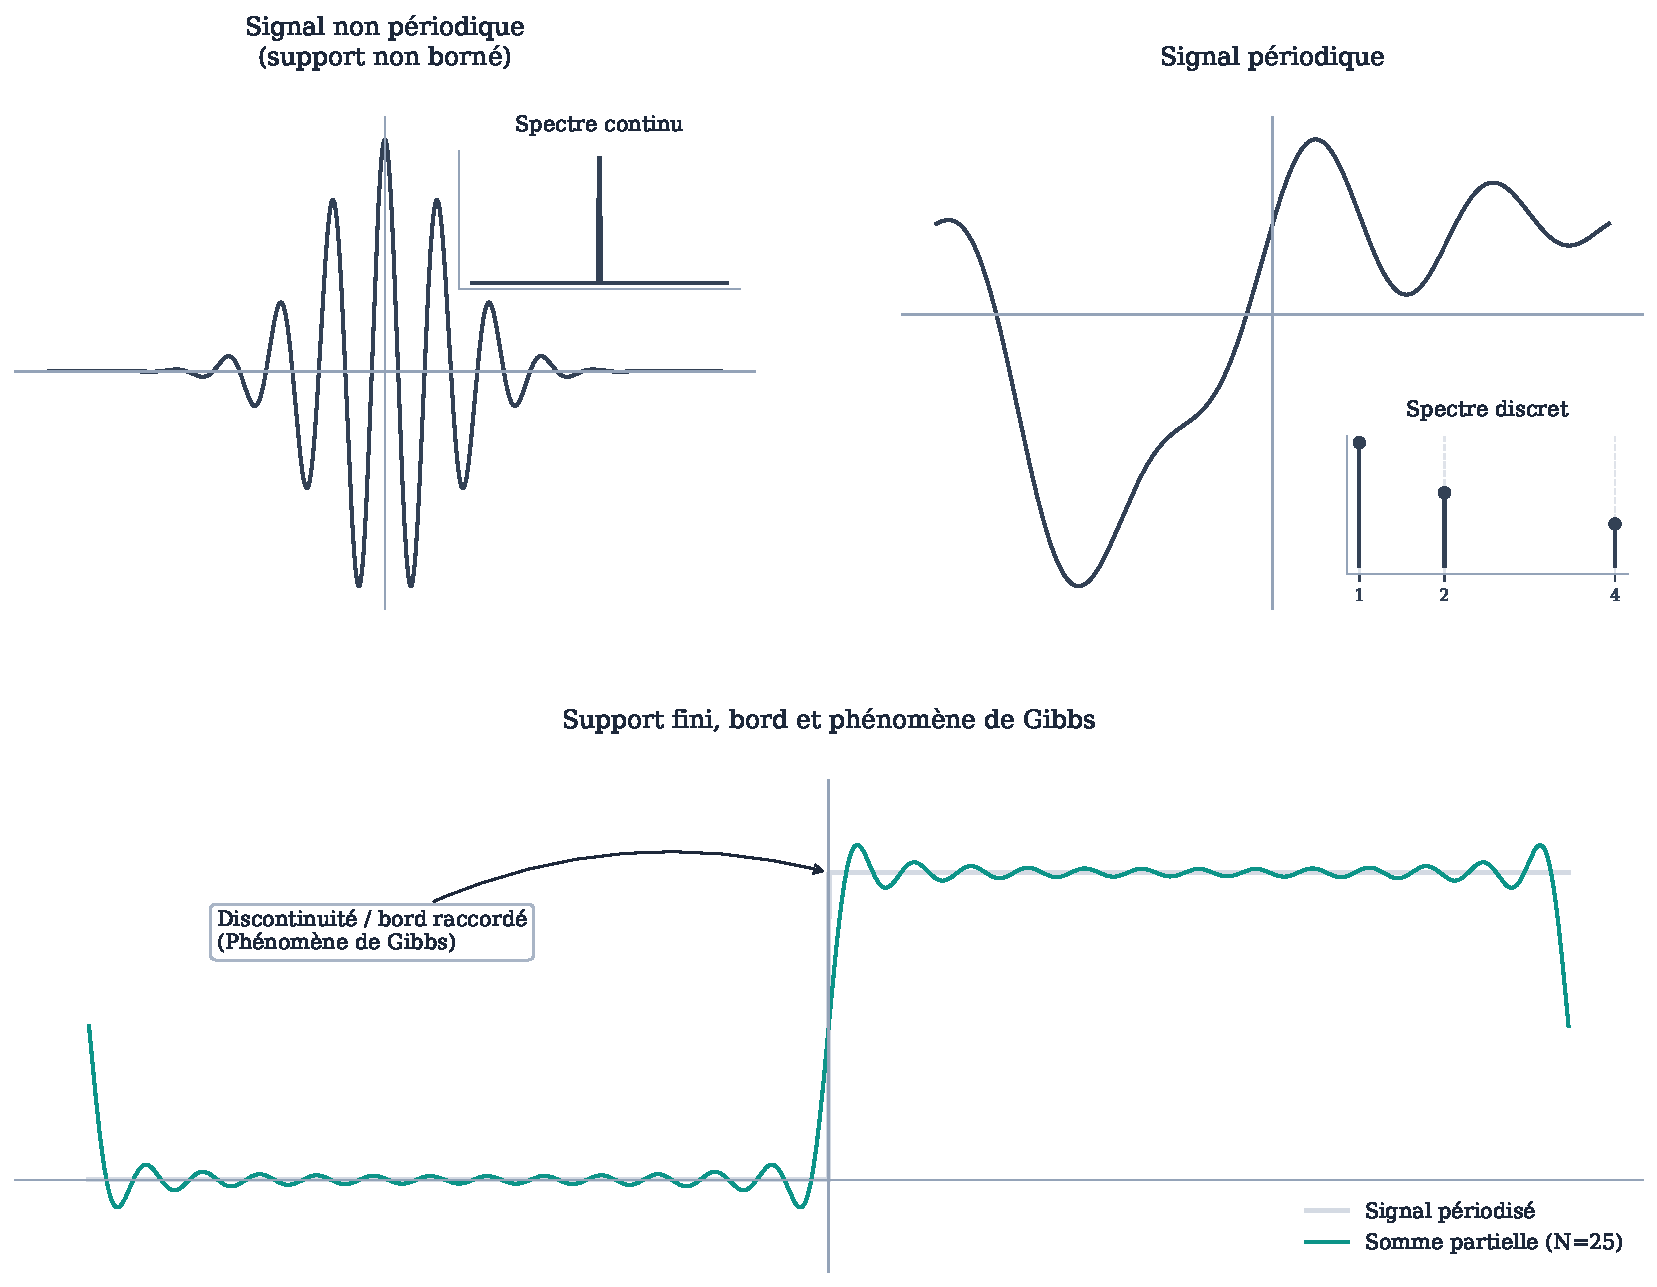
\includegraphics[width=0.8\textwidth]{figures/theory/fourier_periodicite_gibbs.pdf}
    \caption{À gauche : un signal non périodique défini sur un domaine infini possède un spectre continu.
    Au centre : un signal périodique possède un spectre discret constitué de raies harmoniques.
    À droite : un signal de support fini peut présenter une discontinuité artificielle lorsqu'il est périodisé.}
    \label{fig:gibbs}
\end{figure}

\section{Détail de la preuve de la structure BCCB}
\label{app:preuve_bccb}

On reprend ici le cas d'une convolution circulaire 2D mono-canal. L'objectif est de montrer,
pas à pas, pourquoi la matrice $M$ associée à cette convolution est circulante par blocs, 
et chacun de ses blocs est lui-même circulant.

\begin{proof}

On note $X\in\mathbb{C}^{N\times N}$ l'image d'entrée, $Y\in\mathbb{C}^{N\times N}$ l'image de
sortie, et $h\in\mathbb{C}^{N\times N}$ le filtre. On rappelle que dans le cadre circulaire, la convolution 2D s'écrit

$$\begin{aligned}
    Y[m,n] &= \sum_{a=0}^{N-1} \sum_{b=0}^{N-1} h[a,b] \, X[(m-a)\bmod N, \, (n-b)\bmod N] \\
           &= \sum_{a=0}^{N-1} \sum_{b=0}^{N-1} h[(m-a)\bmod N, \, (n-b)\bmod N] \, X[a, b].
\end{aligned}$$

Avec la vectorisation par colonnes, l'entrée $X[r,s]$ correspond à l'indice vectorisé
$r+Ns$, et la sortie $Y[m,n]$ correspond à l'indice vectorisé $m+Nn$. La matrice $M$ est définie
par
\[
    \operatorname{vec}(Y)=M\operatorname{vec}(X).
\]
Le coefficient de $M$ situé à la ligne $m+Nn$ et à la colonne $r+Ns$ indique donc comment le pixel
$X[r,s]$ contribue au pixel $Y[m,n]$.

D'après la formule de convolution 2D, cette contribution est donnée par
\[
    M_{m+Nn,\;r+Ns}
    =
    h[(m-r)\bmod N,\,(n-s)\bmod N].
\]
Cette formule est le point central de la preuve : le coefficient dépend seulement des décalages
circulaires entre les positions d'entrée et de sortie.

On découpe maintenant la matrice $M$ en $N\times N$ blocs, chacun de taille $N\times N$ :
\[
M =
\begin{pmatrix}
B_{0,0} & B_{0,1} & \cdots & B_{0,N-1} \\
B_{1,0} & B_{1,1} & \cdots & B_{1,N-1} \\
\vdots  & \vdots  & \ddots & \vdots \\
B_{N-1,0} & B_{N-1,1} & \cdots & B_{N-1,N-1}
\end{pmatrix}.
\]
Dans ce découpage, le bloc $B_{n,s}$ décrit l'effet de la colonne $s$ de l'image d'entrée sur la
colonne $n$ de l'image de sortie.

Les coefficients de ce bloc sont donc
\[
    (B_{n,s})_{m,r}
    =
    M_{m+Nn,\;r+Ns}
    =
    h[(m-r)\bmod N,\,(n-s)\bmod N].
\]

Fixons maintenant deux colonnes $n$ et $s$. Leur décalage circulaire est
\[
    \delta = (n-s)\bmod N.
\]
Avec cette notation, l'expression précédente devient
\[
    (B_{n,s})_{m,r}
    =
    h[(m-r)\bmod N,\delta].
\]

Pour un $\delta$ fixé, le coefficient $(B_{n,s})_{m,r}$ dépend de $m$ et $r$ uniquement à travers
la différence circulaire $(m-r)\bmod N$. Cela signifie que les lignes du bloc se répètent par
décalage circulaire. Autrement dit, chaque bloc $B_{n,s}$ est une matrice circulante.

Pour rendre cela plus explicite, on définit le vecteur
\[
h_\delta =
\begin{pmatrix}
h[0,\delta] \\
h[1,\delta] \\
\vdots \\
h[N-1,\delta]
\end{pmatrix}.
\]
Le bloc $B_{n,s}$ est alors la matrice circulante construite à partir de ce vecteur :
\[
    B_{n,s}
    =
    C_{h_\delta}.
\]
Comme $\delta=(n-s)\bmod N$, on peut aussi écrire
\[
    B_{n,s}
    =
    C_{h_{(n-s)\bmod N}}.
\]

Cette formule montre maintenant le deuxième niveau de circularité. Lorsque l'on change $n$ et $s$,
les blocs ne changent pas de manière quelconque : ils dépendent seulement du décalage circulaire
$(n-s)\bmod N$. Les blocs eux-mêmes sont donc organisés de manière circulaire.

La matrice complète $M$ peut alors s'écrire sous la forme
\[
M =
\begin{pmatrix}
C_{h_0}     & C_{h_{N-1}} & C_{h_{N-2}} & \cdots & C_{h_1} \\
C_{h_1}     & C_{h_0}     & C_{h_{N-1}} & \cdots & C_{h_2} \\
C_{h_2}     & C_{h_1}     & C_{h_0}     & \cdots & C_{h_3} \\
\vdots      & \vdots      & \vdots      & \ddots & \vdots \\
C_{h_{N-1}} & C_{h_{N-2}} & C_{h_{N-3}} & \cdots & C_{h_0}
\end{pmatrix}.
\]

Cette écriture fait apparaître clairement les deux propriétés recherchées :
\[
    \boxed{\text{chaque bloc est circulant}}
    \qquad\text{et}\qquad
    \boxed{\text{les blocs sont eux-mêmes organisés circulairement}.}
\]
Par conséquent, $M$ est bien une matrice circulante par blocs avec des blocs circulants, c'est-à-dire
une matrice BCCB.

\end{proof}

\section{Détail de la preuve pour les skip connections}
\label{app:preuve_skip_connection}

On reprend ici le cas d'une \textit{skip connection} identité étudié dans la section~\ref{sec:skip-normalisation}. 
L'objectif est de vérifier explicitement que les vecteurs singuliers droits conservent la même structure fréquentielle que dans le cas sans \textit{skip connection}.

\begin{proof}

Soit $a \in \mathbb{C}^m$ un vecteur singulier droit de $G_{\mathrm{skip}}^{(w)}$, associé à une valeur singulière $\sigma$ et à un vecteur singulier gauche $b \in \mathbb{C}^m$ :
\[
G_{\mathrm{skip}}^{(w)}a = \sigma b.
\]

Dans l'espace complet du réseau, on considère le vecteur
\[
v = a \otimes (Q_N)_w.
\]
En utilisant la même notation que précédemment, cela correspond à
\[
v = a \otimes (F_N)_u \otimes (F_N)_v,
\]
où l'indice aplati $w$ correspond au couple de fréquences spatiales $(u,v)$.

Appliquons maintenant l'opérateur $M_{\mathrm{skip}}$ à ce vecteur :
\begin{align*}
M_{\mathrm{skip}}v
&=
(I_m \otimes Q_N)(L + I_{mN^2})(I_m \otimes Q_N)^H
\bigl(a \otimes (Q_N)_w\bigr).
\end{align*}

Comme $(Q_N)_w = Q_N e_w$, on a
\[
a \otimes (Q_N)_w
=
(I_m \otimes Q_N)(a \otimes e_w).
\]
Donc
\begin{align*}
M_{\mathrm{skip}}v
&=
(I_m \otimes Q_N)(L + I_{mN^2})(a \otimes e_w).
\end{align*}

La présence du vecteur canonique $e_w$ sélectionne les coefficients associés à la fréquence $w$. 
Sur cette fréquence, l'opérateur central se comporte comme la matrice de mélange augmentée
\[
G_{\mathrm{skip}}^{(w)} = G^{(w)} + I_m.
\]
Ainsi, l'action sur les canaux et sur la fréquence spatiale se sépare :
\begin{align*}
(L + I_{mN^2})(a \otimes e_w)
&= (G^{(w)}a + I_m a) \otimes e_w \\
&= (G_{\mathrm{skip}}^{(w)}a) \otimes e_w.
\end{align*}

Comme $a$ est un vecteur singulier droit de $G_{\mathrm{skip}}^{(w)}$, on a
\[
G_{\mathrm{skip}}^{(w)}a = \sigma b.
\]
On obtient donc
\[
(L + I_{mN^2})(a \otimes e_w) = \sigma(b \otimes e_w).
\]

En réinjectant ce résultat dans l'expression de $M_{\mathrm{skip}}v$, il vient :
\begin{align*}
M_{\mathrm{skip}}v
&=
(I_m \otimes Q_N) \bigl( \sigma(b \otimes e_w) \bigr) \\
&= \sigma \bigl( (I_m b) \otimes (Q_N e_w) \bigr) \\
&= \sigma\bigl(b \otimes (Q_N)_w\bigr).
\end{align*}

Ainsi, l'application de $M_{\mathrm{skip}}$ au vecteur
\[
v = a \otimes (Q_N)_w
\]
donne bien un vecteur de sortie de même fréquence spatiale :
\[
M_{\mathrm{skip}}v = \sigma\bigl(b \otimes (Q_N)_w\bigr).
\]

La fréquence spatiale $(Q_N)_w$ est donc conservée. Seuls l'amplitude globale, donnée par $\sigma$, et le profil de canaux, donné par $b$, sont modifiés.

Par conséquent, les vecteurs singuliers droits de l'opérateur avec \textit{skip connection} restent de la forme
\[
a \otimes (Q_N)_w,
\]
c'est-à-dire
\[
a \otimes (F_N)_u \otimes (F_N)_v.
\]
\end{proof}

\section{Représentation graphique du stride}

\definecolor{gridblue}{HTML}{006699}
\definecolor{gridteal}{HTML}{148F77}
\definecolor{gridred}{HTML}{E74C3C}
\definecolor{selectgray}{HTML}{D3D3D3}

\begin{figure}[H]
    \centering
    \begin{tikzpicture}[scale=0.75, every node/.style={transform shape}] 

        % =========================================================================
        % GAUCHE : Stride = 1
        % =========================================================================
        \begin{scope}[shift={(0,0)}]
            % Titre parfaitement centré sur l'axe vertical de la figure (x=0)
            \node[font=\large\bfseries] at (0,6.5) {Stride = 1 (Glissement continu)};
            
            \begin{scope}[x={(0.6cm,0.3cm)}, y={(-0.6cm,0.3cm)}, z={(0cm,0.8cm)}]
                
                % --- Image d'entrée 5x5 ---
                \fill[gridblue] (0,0,0) -- (5,0,0) -- (5,5,0) -- (0,5,0) -- cycle;
                \draw[black, thick, join=round] (0,0,0) -- (5,0,0) -- (5,5,0) -- (0,5,0) -- cycle;
                \foreach \i in {1,...,4} {
                    \draw[black, thick] (\i,0,0) -- (\i,5,0);
                    \draw[black, thick] (0,\i,0) -- (5,\i,0);
                }
                
                % --- Filtre initial ---
                \fill[gridred, opacity=0.8] (0,0,0) -- (3,0,0) -- (3,3,0) -- (0,3,0) -- cycle;
                \draw[black, thick, join=round] (0,0,0) -- (3,0,0) -- (3,3,0) -- (0,3,0) -- cycle;
                \foreach \i in {1,2} {
                    \draw[black, thick] (\i,0,0) -- (\i,3,0);
                    \draw[black, thick] (0,\i,0) -- (3,\i,0);
                }

                % --- Mouvement du filtre (Fantôme) ---
                \draw[gridred, ultra thick, dashed, opacity=1] (1,0,0) -- (4,0,0) -- (4,3,0) -- (1,3,0) -- cycle;
                
                % --- Flèche de direction unique (+1) très visible ---
                \draw[->, ultra thick, gridred, line join=round] (1.5,1.5,0) -- (2.5,1.5,0) 
                    node[midway, sloped, below, yshift=-3pt, font=\bfseries\large, fill=white, fill opacity=0.9, text opacity=1, inner sep=3pt, rounded corners=2pt] {+1};
                
                % --- Projection (Pointillés très marqués) ---
                \draw[black!70, very thick, dashed] (0,0,0) -- (1,1,4.5);
                \draw[black!70, very thick, dashed] (3,0,0) -- (2,1,4.5);
                \draw[black!70, very thick, dashed] (3,3,0) -- (2,2,4.5);
                \draw[black!70, very thick, dashed] (0,3,0) -- (1,2,4.5);
                
                % --- Image de sortie 3x3 ---
                \fill[gridteal] (1,1,4.5) -- (4,1,4.5) -- (4,4,4.5) -- (1,4,4.5) -- cycle;
                \draw[black, thick, join=round] (1,1,4.5) -- (4,1,4.5) -- (4,4,4.5) -- (1,4,4.5) -- cycle;
                \foreach \i in {2,3} {
                    \draw[black, thick] (\i,1,4.5) -- (\i,4,4.5);
                    \draw[black, thick] (1,\i,4.5) -- (4,\i,4.5);
                }
                
                \node[anchor=south east, font=\small\bfseries] at (1,4,4.7) {Sortie $3 \times 3$};
            
                % Pixel calculé
                \fill[selectgray, opacity=0.9] (1,1,4.5) -- (2,1,4.5) -- (2,2,4.5) -- (1,2,4.5) -- cycle;
                \draw[black, thick] (1,1,4.5) -- (2,1,4.5) -- (2,2,4.5) -- (1,2,4.5) -- cycle;
                
            \end{scope}
            
            \node[font=\small\bfseries] at (0,-1.5) {Entrée $5 \times 5$};
            
        \end{scope}

        % =========================================================================
        % DROITE : Stride = 2 
        % =========================================================================
        \begin{scope}[shift={(10,0)}] 
            \node[font=\large\bfseries] at (0,6.5) {Stride = 2 (Pas de 2 positions)};

            \begin{scope}[x={(0.6cm,0.3cm)}, y={(-0.6cm,0.3cm)}, z={(0cm,0.8cm)}]
                
                % --- Image d'entrée 5x5 ---
                \fill[gridblue] (0,0,0) -- (5,0,0) -- (5,5,0) -- (0,5,0) -- cycle;
                \draw[black, thick, join=round] (0,0,0) -- (5,0,0) -- (5,5,0) -- (0,5,0) -- cycle;
                \foreach \i in {1,...,4} {
                    \draw[black, thick] (\i,0,0) -- (\i,5,0);
                    \draw[black, thick] (0,\i,0) -- (5,\i,0);
                }
                
                % --- Filtre initial ---
                \fill[gridred, opacity=0.8] (0,0,0) -- (3,0,0) -- (3,3,0) -- (0,3,0) -- cycle;
                \draw[black, thick, join=round] (0,0,0) -- (3,0,0) -- (3,3,0) -- (0,3,0) -- cycle;
                \foreach \i in {1,2} {
                    \draw[black, thick] (\i,0,0) -- (\i,3,0);
                    \draw[black, thick] (0,\i,0) -- (3,\i,0);
                }

                % --- Mouvement du filtre (Fantôme) ---
                \draw[gridred, ultra thick, dashed, opacity=1] (2,0,0) -- (5,0,0) -- (5,3,0) -- (2,3,0) -- cycle;

                % --- Flèche de direction unique (+2) ---
                \draw[->, ultra thick, gridred, line join=round] (1.5,1.5,0) -- (3.5,1.5,0) 
                    node[midway, sloped, below, yshift=-3pt, font=\bfseries\large, fill=white, fill opacity=0.9, text opacity=1, inner sep=3pt, rounded corners=2pt] {+2};

                % --- Projection (Pointillés très marqués) ---
                \draw[black!70, very thick, dashed] (0,0,0) -- (1.5,1.5,4.5);
                \draw[black!70, very thick, dashed] (3,0,0) -- (2.5,1.5,4.5);
                \draw[black!70, very thick, dashed] (3,3,0) -- (2.5,2.5,4.5);
                \draw[black!70, very thick, dashed] (0,3,0) -- (1.5,2.5,4.5);
                
                % --- Image de sortie 2x2 ---
                \fill[gridteal] (1.5,1.5,4.5) -- (3.5,1.5,4.5) -- (3.5,3.5,4.5) -- (1.5,3.5,4.5) -- cycle;
                \draw[black, thick, join=round] (1.5,1.5,4.5) -- (3.5,1.5,4.5) -- (3.5,3.5,4.5) -- (1.5,3.5,4.5) -- cycle;
                \draw[black, thick] (2.5,1.5,4.5) -- (2.5,3.5,4.5);
                \draw[black, thick] (1.5,2.5,4.5) -- (3.5,2.5,4.5);
                
                \node[anchor=south east, font=\small\bfseries] at (1.5,3.5,4.7) {Sortie $2 \times 2$};

                % Pixel calculé
                \fill[selectgray, opacity=0.9] (1.5,1.5,4.5) -- (2.5,1.5,4.5) -- (2.5,2.5,4.5) -- (1.5,2.5,4.5) -- cycle;
                \draw[black, thick] (1.5,1.5,4.5) -- (2.5,1.5,4.5) -- (2.5,2.5,4.5) -- (1.5,2.5,4.5) -- cycle;
                
            \end{scope}
            
            \node[font=\small\bfseries] at (0,-1.5) {Entrée $5 \times 5$};
            
        \end{scope}

        % =========================================================================
        % LÉGENDE 
        % =========================================================================
        \node[anchor=center, draw=black!30, thick, rounded corners, fill=white, inner sep=10pt] at (5,-3.2) {
            \begin{tikzpicture}
                \fill[gridblue] (0,0) rectangle (0.5,0.5); \node[right, font=\small\bfseries] at (0.6,0.25) {Entrée};
                \fill[gridred, opacity=0.8] (3,0) rectangle (3.5,0.5); \node[right, font=\small\bfseries] at (3.6,0.25) {Filtre};
                \fill[gridteal] (6,0) rectangle (6.5,0.5); \node[right, font=\small\bfseries] at (6.6,0.25) {Sortie};
                \fill[selectgray] (9,0) rectangle (9.5,0.5); \node[right, font=\small\bfseries] at (9.6,0.25) {Pixel calculé};
            \end{tikzpicture}
        };

    \end{tikzpicture}
    \caption{Effet du \textit{stride} sur la résolution spatiale de sortie.}
    \label{fig:stride_comparison}
\end{figure}

\section{Illustration de l'average pooling}

\begin{figure}[H]
    \centering
    \begin{tikzpicture}[scale=0.85, transform shape]
        % --- GRILLE D'ENTREE (4x4) ---
        \draw[step=1cm, gray!40, thin] (0,0) grid (4,4);
        
        % Couleurs des blocs 2x2 (Style sobre et epure)
        \fill[blue, opacity=0.08] (0,2) rectangle (2,4);
        \fill[red, opacity=0.08] (2,2) rectangle (4,4);
        \fill[green!60!black, opacity=0.08] (0,0) rectangle (2,2);
        \fill[orange, opacity=0.08] (2,0) rectangle (4,2);

        % Cadres des blocs
        \draw[blue, thick, rounded corners=1pt] (0,2) rectangle (2,4);
        \draw[red, thick, rounded corners=1pt] (2,2) rectangle (4,4);
        \draw[green!60!black, thick, rounded corners=1pt] (0,0) rectangle (2,2);
        \draw[orange, thick, rounded corners=1pt] (2,0) rectangle (4,2);

        % Valeurs d'entree (Exemple numerique simple)
        \foreach \x/\y/\v in {0.5/3.5/1, 1.5/3.5/3, 0.5/2.5/3, 1.5/2.5/5,
                              2.5/3.5/5, 3.5/3.5/7, 2.5/2.5/7, 3.5/2.5/9,
                              0.5/1.5/2, 1.5/1.5/2, 0.5/0.5/1, 1.5/0.5/3,
                              2.5/1.5/8, 3.5/1.5/6, 2.5/0.5/9, 3.5/0.5/9} {
            \node[font=\small, text=black!70] at (\x, \y) {\v};
        }

        % --- FLECHE DE TRANSITION ---
        \draw[->, >=stealth, very thick, black!60] (4.5, 2) -- node[above, font=\footnotesize, text=black] {Moyenne locale} node[below, font=\footnotesize, text=black] {\textit{Stride} $s=2$} (7, 2);

        % --- GRILLE DE SORTIE (2x2) ---
        \begin{scope}[xshift=7.5cm, yshift=1cm]
            \draw[step=1cm, gray!40, thin] (0,0) grid (2,2);
            
            % Couleurs correspondantes
            \fill[blue, opacity=0.08] (0,1) rectangle (1,2);
            \fill[red, opacity=0.08] (1,1) rectangle (2,2);
            \fill[green!60!black, opacity=0.08] (0,0) rectangle (1,1);
            \fill[orange, opacity=0.08] (1,0) rectangle (2,1);

            % Valeurs calculees (moyennes)
            \node[font=\bfseries, text=blue!80!black] at (0.5, 1.5) {3};
            \node[font=\bfseries, text=red!80!black] at (1.5, 1.5) {7};
            \node[font=\bfseries, text=green!50!black] at (0.5, 0.5) {2};
            \node[font=\bfseries, text=orange!80!black] at (1.5, 0.5) {8};
        \end{scope}

    \end{tikzpicture}
    \caption{Illustration spatiale de l'opération d'\textit{average pooling}. Chaque bloc de $2 \times 2$ pixels de l'image d'entrée est remplacé par sa moyenne arithmétique, réduisant ainsi la résolution spatiale par un facteur $s=2$.}
    \label{fig:avg_pooling_spatial}
\end{figure}

\section{Rappel sur la SVD et les directions d'amplification}
\label{app:svd-sensibilite}

Soit
\[
    M \in \mathbb{C}^{m_{\mathrm{out}}N^2 \times m_{\mathrm{in}}N^2}
\]
la matrice représentant un opérateur de convolution multi-canaux. Comme cette matrice n'est pas
nécessairement carrée, on utilise la décomposition en valeurs singulières plutôt qu'une diagonalisation
classique par valeurs propres.

La décomposition en valeurs singulières de $M$ s'écrit
\[
    M = U \Sigma V^H,
\]
où $U$ et $V$ sont des matrices unitaires, et où $\Sigma$ est une matrice diagonale rectangulaire
contenant les valeurs singulières de $M$ :
\[
    \sigma_1 \geq \sigma_2 \geq \cdots \geq 0.
\]
Les colonnes de $V$ sont appelées vecteurs singuliers droits de $M$ : elles vivent dans l'espace
d'entrée. Les colonnes de $U$ sont appelées vecteurs singuliers gauches de $M$ : elles vivent dans
l'espace de sortie.

Pour comprendre pourquoi les vecteurs singuliers droits décrivent les directions d'amplification,
on considère la matrice auto-adjointe positive $M^H M$. À partir de la SVD, on obtient
\[
    M^H M
    =
    (U\Sigma V^H)^H(U\Sigma V^H).
\]
En utilisant $(ABC)^H = C^H B^H A^H$, il vient
\[
    M^H M
    =
    V\Sigma^H U^H U \Sigma V^H.
\]
Comme $U$ est unitaire, on a $U^H U = I$, donc
\[
    M^H M
    =
    V\Sigma^H \Sigma V^H.
\]
La matrice $\Sigma^H\Sigma$ est diagonale et contient les carrés des valeurs singulières :
\[
    \Sigma^H\Sigma
    =
    \operatorname{diag}(\sigma_1^2,\sigma_2^2,\dots).
\]
Ainsi,
\[
    M^H M
    =
    V
    \operatorname{diag}(\sigma_1^2,\sigma_2^2,\dots)
    V^H.
\]
Cela montre que les vecteurs singuliers droits de $M$ sont exactement les vecteurs propres de
$M^H M$, et que les valeurs propres associées sont les carrés des valeurs singulières.

En particulier, si $v_i$ désigne la $i$-ème colonne de $V$, alors
\[
    M^H M v_i
    =
    V D V^H v_i
    =
    V D e_i
    =
    V(\sigma_i^2 e_i)
    =
    \sigma_i^2 v_i,
\]
où
\[
    D=\operatorname{diag}(\sigma_1^2,\sigma_2^2,\dots).
\]
Ainsi,
\[
    M^H M v_i = \sigma_i^2 v_i.
\]

De manière équivalente, la valeur singulière $\sigma_i$ mesure l'amplification induite par $M$
dans la direction $v_i$. En effet,
\[
    \|Mv_i\|_2^2
    =
    (Mv_i)^H(Mv_i)
    =
    v_i^H M^H M v_i
    =
    v_i^H(\sigma_i^2 v_i)
    =
    \sigma_i^2 \|v_i\|_2^2.
\]
Comme $V$ est unitaire, ses colonnes forment une base orthonormée. En particulier,
\[
    \|v_i\|_2 = 1.
\]
On obtient donc
\[
    \|Mv_i\|_2 = \sigma_i.
\]

La plus grande valeur singulière décrit l'amplification maximale de $M$ parmi les entrées de norme
$1$ :
\[
    \sigma_1
    =
    \max_{\|x\|_2=1}\|Mx\|_2.
\]
Si $\sigma_1$ est simple, la direction qui réalise cette amplification maximale est le vecteur singulier
droit $v_1$. Si $\sigma_1$ est multiple, il n'y a pas une seule direction maximale : toute direction
unitaire dans le sous-espace associé à $\sigma_1$ donne la même amplification.

Dans le cadre de l'analyse fréquentielle des convolutions, les directions de forte sensibilité du réseau
correspondent donc aux vecteurs singuliers droits associés aux grandes valeurs singulières.

\section{Spectre de Fourier moyen des images propres}
\label{annexe:spectres_moyens_cifar}

Cette annexe présente le spectre de Fourier moyen des images non perturbées de CIFAR-10 et CIFAR-100.
L'objectif n'est pas de mesurer directement la sensibilité du modèle, mais d'observer quelles fréquences
sont naturellement présentes dans les données d'entrée.

\begin{figure}[H]
    \centering
    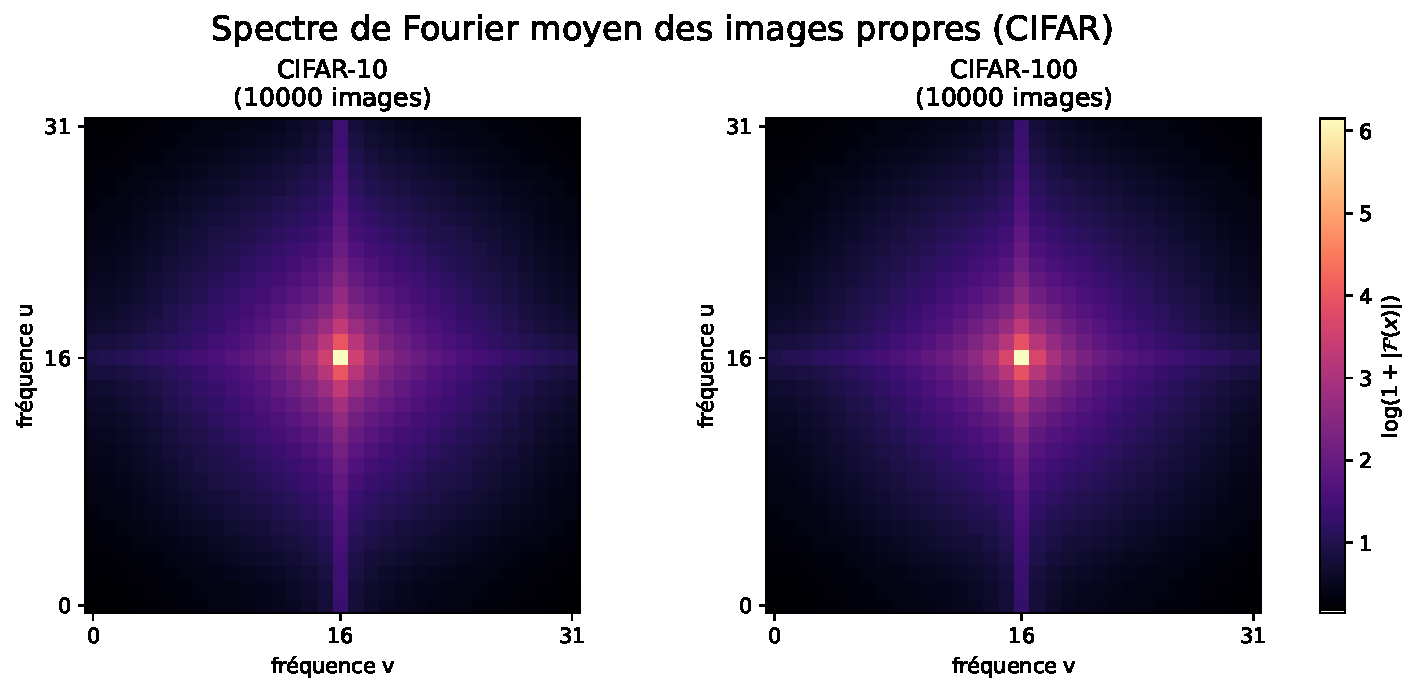
\includegraphics[width=\textwidth]{figures/results/mean_clean_spectrum_comparison_cifar.pdf}
    \caption{Spectre de Fourier moyen des images non perturbées de CIFAR-10 et CIFAR-100. Les valeurs affichées
    correspondent à $\log(1+|\mathcal{F}(x)|)$, moyennées sur les images du dataset.}
    \label{fig:mean_clean_spectrum_comparison_cifar}
\end{figure}

On observe que les deux datasets possèdent une structure fréquentielle très similaire : 
l'énergie est fortement concentrée autour du centre du spectre et décroît progressivement selon une forme 
proche d'un losange. Les lignes horizontale et verticale plus marquées indiquent également que certaines 
directions fréquentielles sont plus présentes que d'autres dans les images non perturbées.

Cette observation fournit une piste d'interprétation pour les heatmaps SFA. Elle montre que les images
d'entrée possèdent elles-mêmes une organisation fréquentielle non uniforme. La sensibilité du modèle
peut donc dépendre à la fois de l'architecture et des statistiques des données utilisées pendant
l'entraînement.

Cette comparaison reste toutefois descriptive. Le spectre moyen caractérise les images d'entrée, alors
que les heatmaps SFA mesurent la réponse du modèle à des perturbations imposées. Les deux objets ne
doivent donc pas être confondus.

\section{Analyse complémentaire : rôle du mélange des canaux dans la SFA}
\label{annexe:color_sfa}

Dans le cadre théorique présenté au chapitre précédent, les directions singulières d'un modèle
convolutionnel linéarisé peuvent s'écrire sous une forme du type
\[
    v = a \otimes q_{u,v},
\]
où \(q_{u,v}\) représente une composante spatiale de Fourier et où
\(a \in \mathbb{R}^3\) décrit le mélange entre les canaux rouge, vert et bleu.

La \textit{Single Fourier Attack} utilisée dans le protocole principal simplifie ce cadre. Elle ne cherche
pas à optimiser simultanément la fréquence spatiale et le vecteur couleur \(a\). Le même motif de
Fourier est appliqué aux trois canaux RGB, ce qui revient à utiliser le vecteur
\[
    a_{\mathrm{uni}} = (1,1,1).
\]
L'espace de recherche est donc réduit au choix de la fréquence $(u,v)$. Cette simplification
rend l'attaque beaucoup plus simple à évaluer, puisqu'il suffit de parcourir les fréquences du
domaine de Fourier. Elle est également cohérente avec la contrainte $\ell_\infty$ utilisée dans
le protocole principal : le motif est appliqué avec l'amplitude maximale autorisée sur chacun des
trois canaux.

Nous distinguons alors deux manières de contraindre le mélange entre canaux. La première
conserve une contrainte comparable à la SFA standard en norme $\ell_\infty$, afin de tester si
un autre choix de direction couleur peut améliorer l'attaque à amplitude maximale identique. La
seconde utilise un budget de type $\ell_1$ sur les coefficients du vecteur couleur. Dans ce cas,
un vecteur comme $a=(3,0,0)$ est possible : le budget total est concentré sur un seul canal, ce
qui ne correspond plus exactement à la contrainte de la SFA standard. Les deux variantes ne
mesurent donc pas exactement la même chose ; elles servent plutôt à tester si le choix du mélange
RGB peut renforcer l'effet d'une fréquence de Fourier.

\subsection*{Recherche de vecteurs RGB par fréquence}

La figure~\ref{fig:color_sfa_foolratio_and_activation_grids} compare la SFA standard avec des variantes
où le vecteur RGB \(a\) est choisi parmi un ensemble restreint de combinaisons possibles.

\begin{figure}[H]
    \centering
    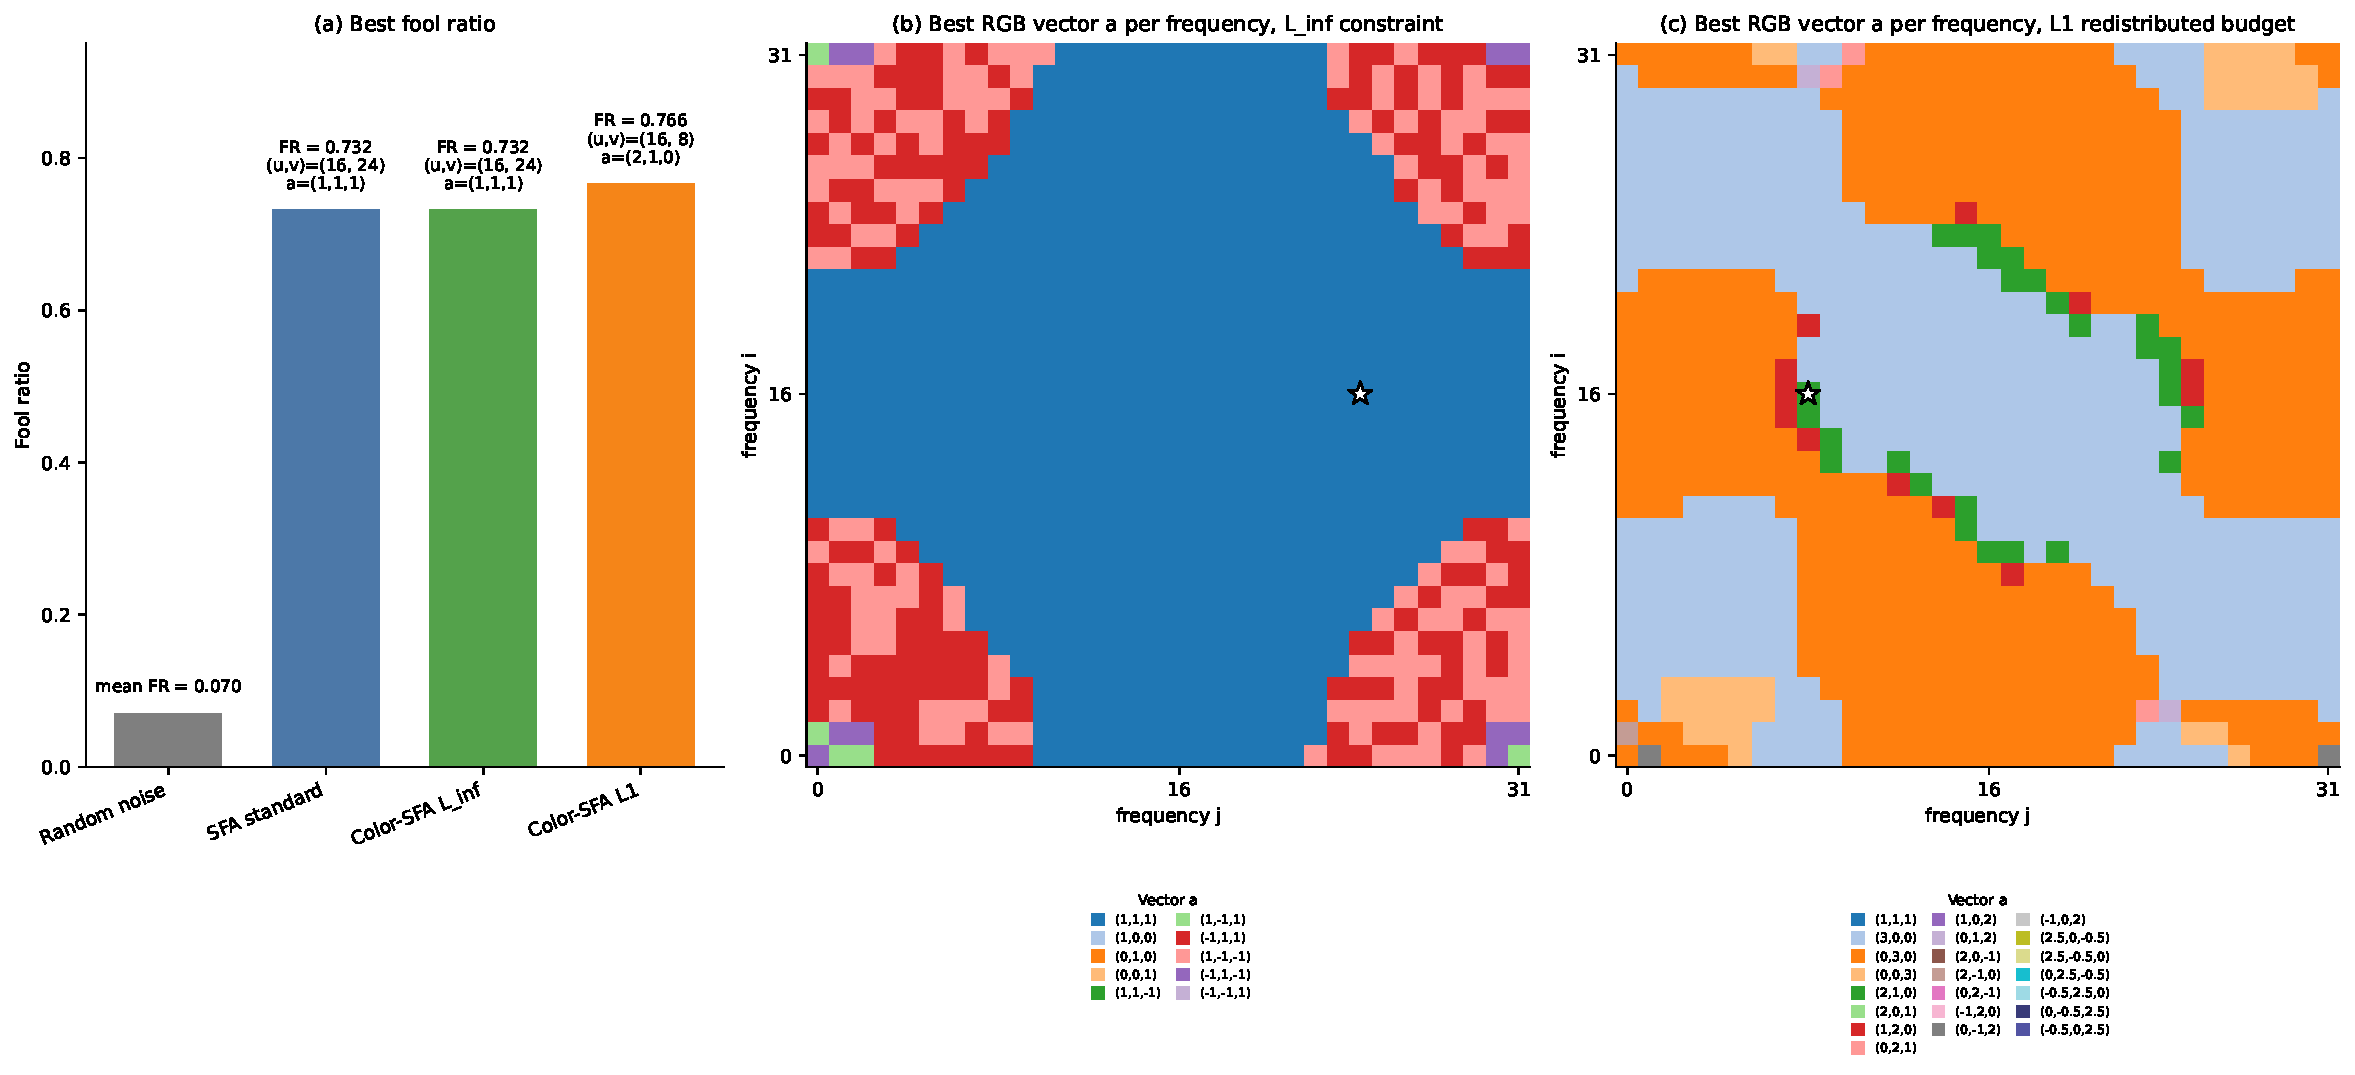
\includegraphics[width=\textwidth]{figures/results/color_sfa_foolratio_and_activation_grids.pdf}
    \caption{Comparaison entre la SFA standard et des variantes où le vecteur RGB \(a\) est choisi par fréquence.
    À gauche, le meilleur \textit{fool ratio} obtenu par chaque méthode est comparé à la baseline de bruit
    aléatoire. Au centre et à droite, chaque case indique le meilleur vecteur RGB trouvé pour la fréquence
    correspondante, selon deux contraintes de budget différentes.}
    \label{fig:color_sfa_foolratio_and_activation_grids}
\end{figure}

Dans la variante renormalisée en norme $\ell_\infty$, la meilleure variante colorée retrouve
pratiquement le même résultat que la SFA standard. Ce qui indique que, sous cette contrainte, le
choix d'un mélange RGB différent n'améliore pas significativement l'attaque par rapport à la
direction uniforme $(1,1,1)$.

Avec la variante sous budget $\ell_1$ sur les coefficients couleur, le meilleur score augmente légèrement,
passant d'environ \(0.732\) à \(0.766\), avec la fréquence \((16,8)\) et le vecteur \(a=(2,1,0)\).
Ce qui est assez modeste dans notre cas.

\subsection*{Comparaison de directions couleur fixes}

Nous avons ensuite comparé plusieurs directions couleur simples :
\[
(1,1,1), \quad (1,0,0), \quad (0,1,0), \quad (0,0,1),
\]
ainsi que des directions chromatiques opposées :
\[
(1,-1,0), \quad (1,0,-1), \quad (0,1,-1),
\]
et une direction de type luminance.

Les résultats de la figure~\ref{fig:color_sfa_cifar10} montrent que la direction standard
$(1,1,1)$ reste nettement la plus efficace. Les directions appliquées à un seul canal ont un effet
plus faible, tandis que les directions chromatiques opposées $(1,-1,0)$, $(1,0,-1)$ et
$(0,1,-1)$ donnent des fool ratios presque nuls.

\begin{figure}[H]
    \centering
    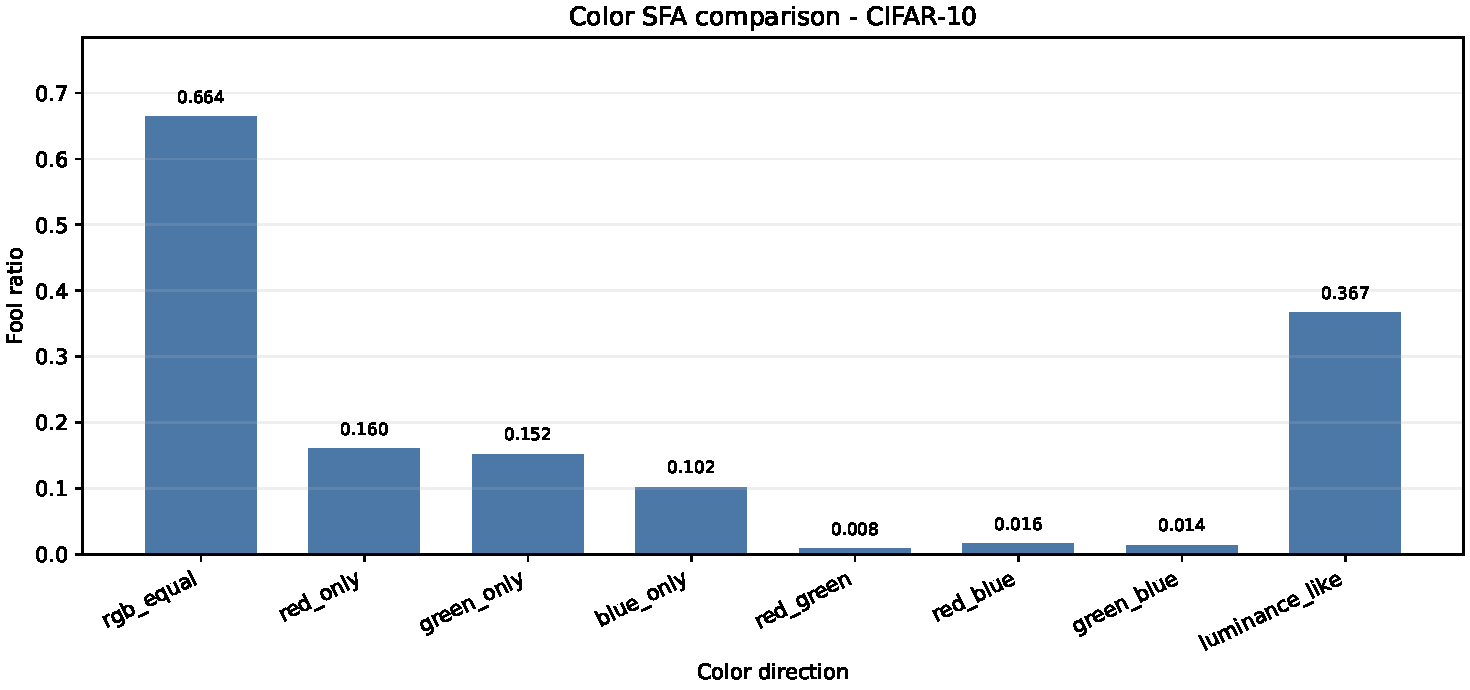
\includegraphics[width=0.85\textwidth]{figures/results/color_sfa_cifar10_barplot.pdf}
    \caption{Comparaison de plusieurs directions couleur pour la \textit{Single Fourier Attack}
    sur CIFAR-10.}
    \label{fig:color_sfa_cifar10}
\end{figure}

Cette observation suggère que, pour la fréquence étudiée, les directions chromatiques opposées
sont faiblement transmises par le réseau. Nous pouvons l'interpréter à partir du cadre
multi-canaux. Pour une fréquence fixée $(u,v)$, l'effet d'une direction couleur
$a \in \mathbb{R}^3$ est décrit par la matrice de mélange $G^{(u,v)}$ :
\[
    \beta = G^{(u,v)}a.
\]
La SFA standard correspond au choix
\[
    a_{\mathrm{uni}} = (1,1,1),
\]
c'est-à-dire à une variation commune des trois canaux RGB.

\paragraph{Cas idéalement symétrique.}
Supposons que, pour la fréquence considérée, le réseau réponde de la même manière aux trois
canaux d'entrée. Cela revient à supposer que les trois colonnes de $G^{(u,v)}$ sont identiques :
\[
    G^{(u,v)}
    =
    \begin{pmatrix}
    | & | & | \\
    g & g & g \\
    | & | & |
    \end{pmatrix}
    =
    g
    \begin{pmatrix}
    1 & 1 & 1
    \end{pmatrix},
\]
où $g \in \mathbb{C}^{m_{\mathrm{out}}}$ décrit la réponse fréquentielle commune du réseau.

Alors, pour toute direction couleur $a=(a_R,a_G,a_B)$, on obtient
\[
    G^{(u,v)}a
    =
    g(a_R+a_G+a_B).
\]
L'amplification dépend donc uniquement de la somme des composantes de $a$. Sous une contrainte
$\ell_\infty$ comparable à celle de la SFA standard,
\[
    |a_R|, |a_G|, |a_B| \leq 1,
\]
cette somme est maximale en valeur absolue pour
\[
    a=(1,1,1)
\]
ou pour son opposé. Ainsi, dans ce cadre symétrique simplifié, la direction uniforme
$a_{\mathrm{uni}}$ est optimale.

Inversement, toute direction couleur vérifiant
\[
    a_R+a_G+a_B=0
\]
est annulée par $G^{(u,v)}$. C'est le cas des directions chromatiques opposées
\[
    (1,-1,0), \qquad (1,0,-1), \qquad (0,1,-1).
\]
Dans ce modèle simplifié, ces directions appartiennent donc au noyau de la matrice de mélange
fréquentielle :
\[
    G^{(u,v)}a = 0.
\]

\paragraph{Cas approximativement symétrique.}
Dans un réseau réel, les colonnes de $G^{(u,v)}$ ne sont pas exactement identiques. On peut
cependant séparer une composante commune aux trois canaux et un terme résiduel :
\[
    G^{(u,v)}
    =
    g
    \begin{pmatrix}
    1 & 1 & 1
    \end{pmatrix}
    + E,
\]
où l'on peut prendre
\[
    g
    =
    \frac{1}{3}G^{(u,v)}
    \begin{pmatrix}
    1 \\ 1 \\ 1
    \end{pmatrix}.
\]
Le terme $E$ mesure alors l'écart à une réponse parfaitement commune aux trois canaux.

Pour une direction chromatique opposée telle que $a_R+a_G+a_B=0$, la composante commune
disparaît :
\[
    G^{(u,v)}a = Ea.
\]
Ainsi, si $\|E\|$ est faible, alors
\[
    \|G^{(u,v)}a\|_2
    \leq
    \|E\|\,\|a\|_2.
\]
Les directions chromatiques opposées ne sont donc plus annulées exactement, mais elles restent
faiblement transmises lorsque le mélange fréquentiel entre les canaux est proche d'une réponse
commune.

Cette proposition fournit une interprétation théorique des résultats observés dans la
figure~\ref{fig:color_sfa_cifar10}. La forte efficacité de $(1,1,1)$ suggère que la fréquence
étudiée active principalement une direction commune aux canaux, tandis que les faibles scores
des directions chromatiques opposées peuvent s'expliquer par une quasi-annulation dans le
mélange fréquentiel des canaux.

\section{Heatmaps internes par couche}
\label{annexe:heatmaps_internes_couches}

En complément de l'analyse d'amplification présentée dans le chapitre principal, nous visualisons ici
l'effet des perturbations de Fourier à différents niveaux internes du réseau. Pour chaque fréquence,
nous mesurons la variation moyenne normalisée des activations après perturbation, puis nous la
comparons au \textit{fool ratio} final.

\begin{figure}[H]
    \centering
    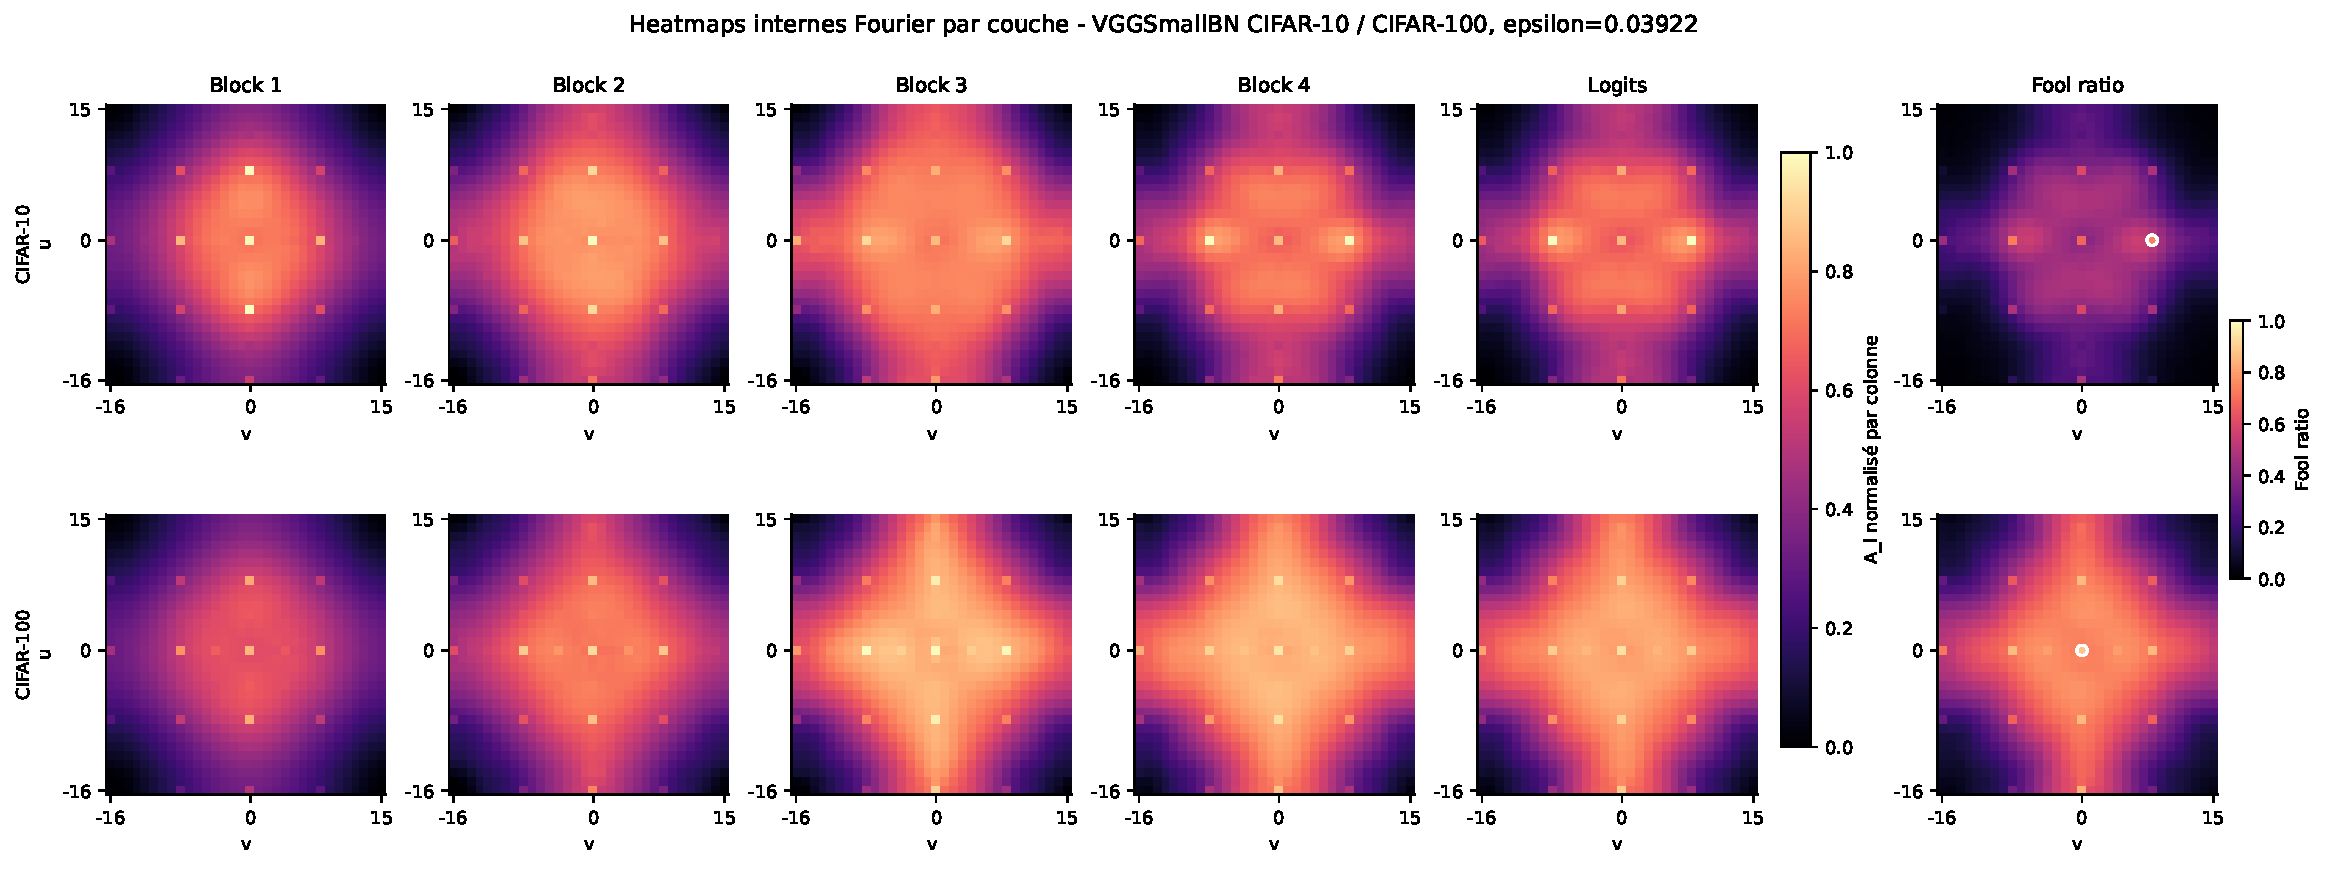
\includegraphics[width=\textwidth]{figures/results/layerwise_fourier_heatmaps_comparison_vgg_cifar10_cifar100.pdf}
    \caption{Heatmaps internes par couche pour \texttt{VGGSmallBN} sur CIFAR-10 et CIFAR-100.
    Les premières colonnes représentent la variation moyenne normalisée des activations internes après
    perturbation de Fourier. La dernière colonne indique le \textit{fool ratio} final.}
    \label{fig:annexe_layerwise_fourier_heatmaps}
\end{figure}

Ces visualisations montrent que la structure fréquentielle observée dans les heatmaps finales apparaît
déjà dans les représentations internes du réseau. Elle devient plus marquée dans les blocs profonds et
dans les logits, ce qui suggère que certaines fréquences sont progressivement amplifiées au cours du
traitement convolutionnel.

\section{Analyse complémentaire des marges logits et des frontières locales}
\label{annexe:marges-logits}

Cette annexe complète l'analyse expérimentale du chapitre~4. L'objectif est de mieux comprendre
pourquoi le modèle entraîné sur CIFAR-100 apparaît plus fragile que celui entraîné sur CIFAR-10.

\subsection{Distribution des marges logits}

Pour chaque image du jeu de test, on calcule les logits produits par le modèle. On note ensuite
$z_{(1)}$ le plus grand logit et $z_{(2)}$ le deuxième plus grand logit. La marge logit est définie par
\[
    m(x) = z_{(1)}(x) - z_{(2)}(x).
\]

Cette quantité mesure basiquement l'écart entre la classe prédite et la classe concurrente la plus proche selon
le modèle.

La figure~\ref{fig:logit-margin-histograms} compare les distributions des marges logits pour
VGGSmallBN sur CIFAR-10 et CIFAR-100. On observe que la distribution de CIFAR-100 est
nettement plus concentrée vers les faibles marges. La médiane est d'environ $4.15$ pour CIFAR-100,
contre environ $11.12$ pour CIFAR-10. Cela signifie que, sur CIFAR-100, les prédictions du modèle
sont en moyenne moins fortement séparées de leur seconde meilleure classe.

\begin{figure}[H]
    \centering
    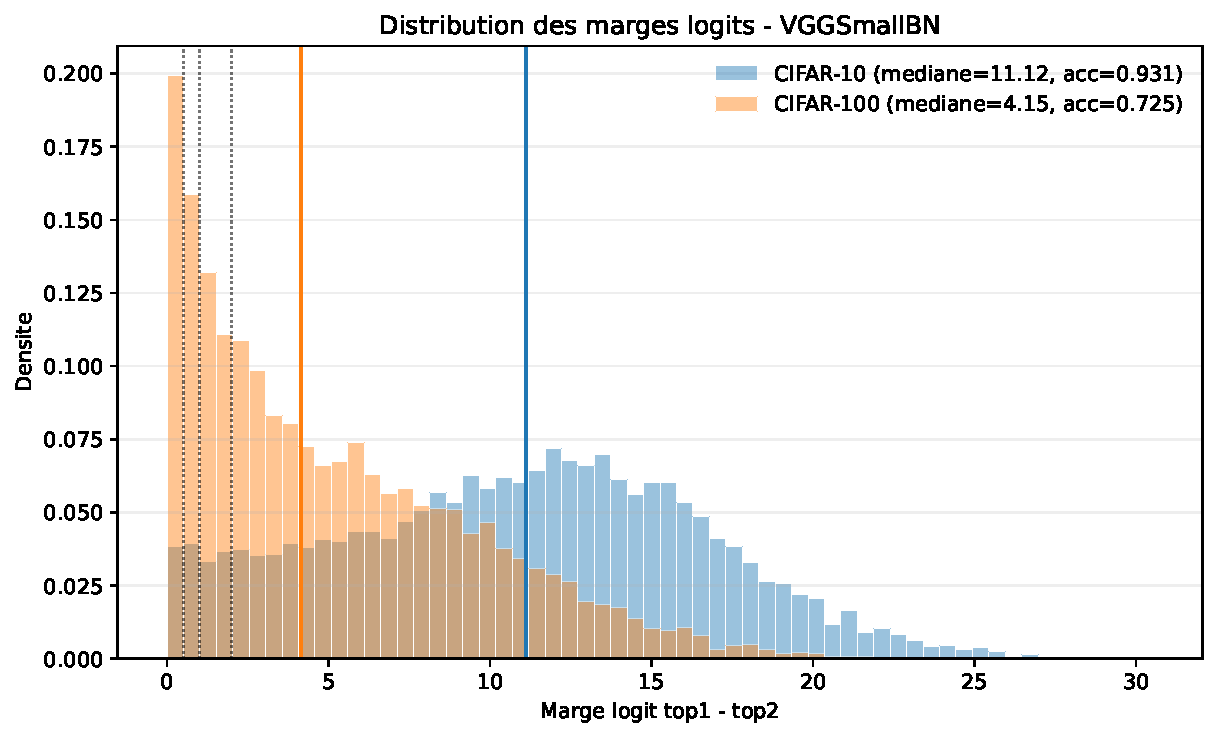
\includegraphics[width=0.85\textwidth]{figures/results/logit_margin_histograms_cifar10_cifar100.pdf}
    \caption{Distribution des marges logits pour VGGSmallBN sur CIFAR-10 et CIFAR-100. La marge est définie comme la différence entre le plus grand logit et le deuxième plus grand logit.}
    \label{fig:logit-margin-histograms}
\end{figure}

Ce résultat donne un appui supplémentaire à l'interprétation proposée dans le chapitre~4 :
la plus grande fragilité observée sur CIFAR-100 ne vient pas seulement du choix d'une fréquence
particulière, mais aussi du fait que les décisions du modèle semblent moins séparées. 

% \subsection{Carte moyenne de stabilité locale}

% En complément de l'analyse des marges logits, nous construisons une carte moyenne de stabilité
% locale autour des images correctement classées. L'objectif est de visualiser, dans une coupe
% bidimensionnelle de l'espace d'entrée, dans quelle mesure les prédictions restent stables lorsque
% l'on perturbe les images selon deux directions fréquentielles sensibles.

% Pour une image $x$, on considère les perturbations de la forme
% \[
%     x_{\alpha,\beta}
%     =
%     x + \alpha d_1 + \beta d_2,
% \]
% où $d_1$ correspond à la direction SFA principale du dataset, et $d_2$ à une seconde direction
% fréquentielle sensible.

% Pour chaque point $(\alpha,\beta)$ de la grille, nous calculons la proportion d'images pour
% lesquelles la prédiction reste identique à celle de l'image propre :
% \[
%     P_{\mathrm{same}}(\alpha,\beta)
%     =
%     \frac{1}{M}
%     \sum_{k=1}^{M}
%     \mathbf{1}\left[
%         f(x_k+\alpha d_1+\beta d_2)=f(x_k)
%     \right].
% \]
% Cette quantité vaut $1$ lorsque toutes les images gardent la même prédiction, et $0$ lorsque
% toutes les prédictions changent. Elle fournit donc une mesure moyenne de la stabilité locale du
% modèle dans la coupe considérée.

% Les cartes sont calculées sur $500$ images correctement classées par dataset, avec une grille
% de taille $41\times 41$.

% \begin{figure}[H]
%     \centering
%     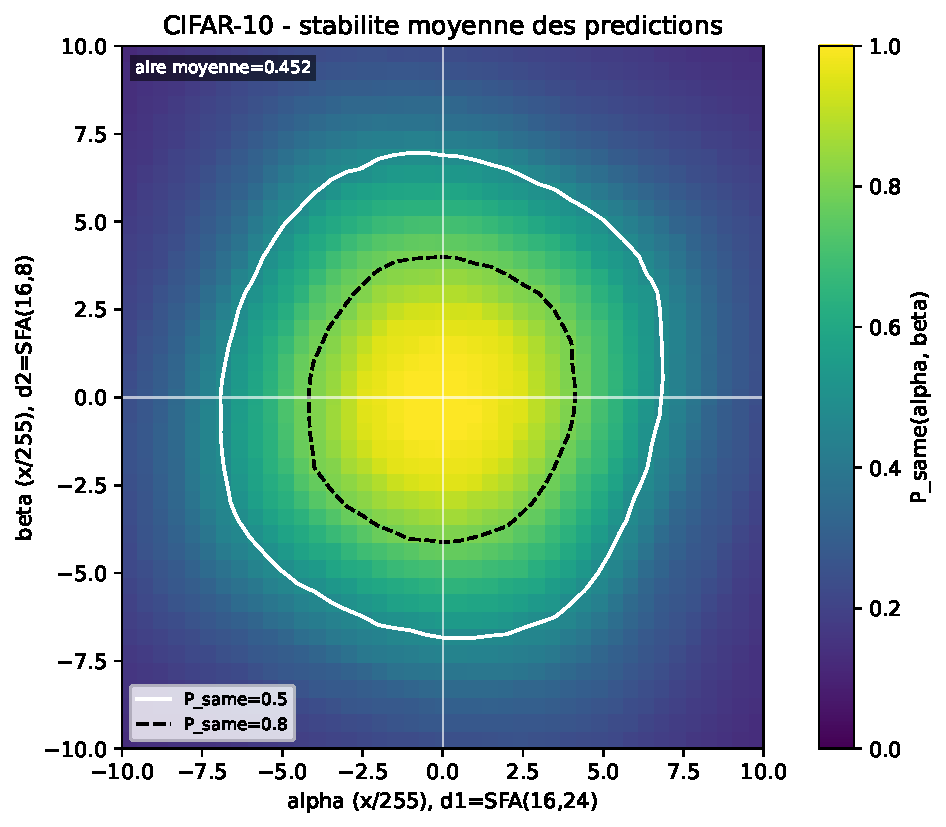
\includegraphics[width=0.48\textwidth]{figures/results/average_decision_boundary_cifar10.pdf}
%     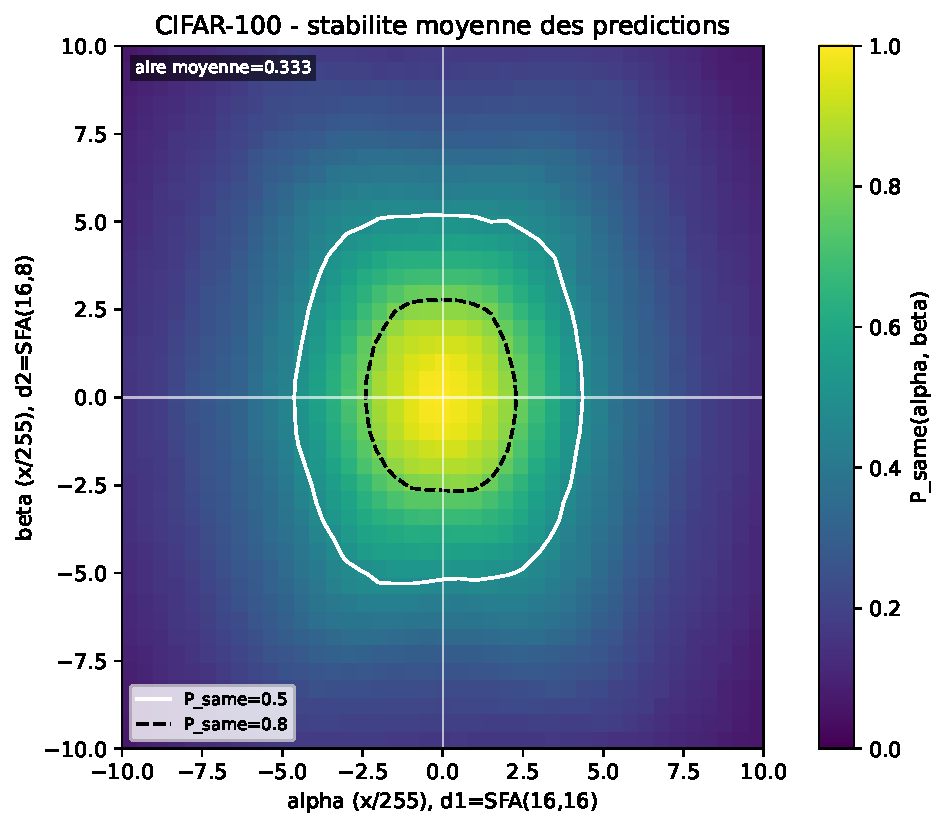
\includegraphics[width=0.48\textwidth]{figures/results/average_decision_boundary_cifar100.pdf}
%     \caption{Cartes moyennes de stabilité locale pour VGGSmallBN sur CIFAR-10 et CIFAR-100. Chaque point indique la proportion d'images dont la prédiction reste inchangée après perturbation selon deux directions fréquentielles sensibles.}
%     \label{fig:average-decision-boundary}
% \end{figure}

% \begin{table}[H]
%     \centering
%     \begin{tabular}{lcccc}
%         \toprule
%         Dataset & Aire stable moyenne & Largeur $P_{\mathrm{same}}\geq 0.5$ & Largeur $P_{\mathrm{same}}\geq 0.8$ & $\alpha$ critique moyen \\
%         \midrule
%         CIFAR-10  & 0.4518 & $13.00/255$ & $8.00/255$ & $5.81/255$ \\
%         CIFAR-100 & 0.3330 & $8.50/255$  & $4.00/255$ & $4.46/255$ \\
%         \bottomrule
%     \end{tabular}
%     \caption{ Les largeurs sont mesurées sur la ligne $\beta=0$, avec Les coefficients $\alpha$ et 
%     $\beta$ qui varient dans l'intervalle $[-10/255,10/255]$}
%     \label{tab:average-decision-boundary}
% \end{table}

% Les résultats du tableau~\ref{tab:average-decision-boundary} montrent que la région moyenne de
% stabilité est plus réduite sur CIFAR-100 que sur CIFAR-10. L'aire stable moyenne passe de
% $0.4518$ à $0.3330$, et la largeur de la région stable le long de la direction SFA diminue également.
% Pour le seuil $P_{\mathrm{same}}\geq 0.8$, cette largeur est divisée par deux, passant de $8.00/255$
% sur CIFAR-10 à $4.00/255$ sur CIFAR-100.

% Cette observation est cohérente avec les résultats principaux du chapitre~4 : le modèle entraîné
% sur CIFAR-100 est globalement plus sensible aux perturbations fréquentielles. Elle complète
% également l'analyse des marges logits, en montrant que cette fragilité se manifeste aussi dans
% une coupe locale de l'espace d'entrée.

% Il faut toutefois rester prudent dans l'interprétation. Ces cartes ne représentent pas la frontière
% de décision complète du réseau, qui vit dans un espace de dimension $32\times32\times3$.
% Elles décrivent seulement une coupe bidimensionnelle construite à partir de deux directions
% fréquentielles sensibles. Elles doivent donc être lues comme une visualisation complémentaire,
% et non comme une preuve complète de la géométrie globale des frontières de décision.

\bibliographystyle{plain}
\bibliography{formalisme/references}

\end{document}
